\documentclass{article}

% Loading packages that alter the style
\usepackage[]{graphicx}
\usepackage[]{color}
\usepackage{alltt}
\usepackage[T1]{fontenc}
\usepackage[utf8]{inputenc}

% Math
\usepackage{amsmath}
\usepackage{amssymb}
\DeclareMathOperator{\argmin}{argmin}
\DeclareMathOperator{\argmax}{argmax}

% Algorithms
\usepackage[ruled]{algorithm2e}
\DontPrintSemicolon
\SetKwInput{KwInput}{Input} % Set the Input
\SetKwInput{KwOutput}{Output}% set the Output


% Fonts
\usepackage{sectsty}
\def\@seccntformat#1{\#\csname the#1\endcsname \quad} %Active Tabor-font with \cs

\sectionfont{\centering\sc\Large}
\subsectionfont{\centering\sc\large\noindent}
\subsubsectionfont{\sc\normalsize}
\paragraphfont{\sc\normalsize}
\subparagraphfont{\sc\small}

\renewcommand{\rmdefault}{ptm}
\renewcommand{\sfdefault}{phv}

% Paragraph setup
\usepackage{indentfirst}
\usepackage[skip=1\baselineskip plus 2pt]{parskip}
%\setlength{\parskip}{\smallskipamount}
%\setlength{\parindent}{12pt}

% Set page margins
%\usepackage[top=3.0cm,bottom=3.0cm,left=2.0cm,right=2.0cm]{geometry}
\usepackage{geometry}
\linespread{1.3} %This makes 1.5 line spacing (yeah, 1.3=1.5).
\usepackage{subcaption}

% Prevents LaTeX from filling out a page to the bottom
\raggedbottom

% Format table of contents
\setcounter{secnumdepth}{3} % How many levels of sections
\setcounter{tocdepth}{3} % How many levels to include in table of contents
%\usepackage{tocloft}
%\cftsetindents{section}{0em}{2em}
%\cftsetindents{subsection}{2em}{2em}

% Adding languages
\usepackage[english]{babel}

% All page numbers positioned at the bottom of the page
\usepackage{fancyhdr}
\fancyhf{} % clear all header and footers
\fancyfoot[C]{\thepage}
\pagestyle{fancy}


% Adds table captions above the table per default
\usepackage{booktabs} % compatible with Pandas
\usepackage{float}
\floatstyle{plaintop}
\restylefloat{table}
\usepackage[tableposition=top]{caption} % Space between caption and table

% Figure format
\usepackage[labelfont=bf]{caption} % Caption in bold
%\numberwithin{equation}{subsection}
%\numberwithin{figure}{subsection}
%\numberwithin{table}{subsection}


% Adds hyperlinks to references and ToC
\usepackage[backref=page]{hyperref} % hyperlinks
\renewcommand*{\backref}[1]{}
\renewcommand*{\backrefalt}[4]{{\footnotesize [%
		\ifcase #1 Not cited.%
		\or Cited on page~#2%
		\else Cited on pages #2%
		\fi%
		]}}
\usepackage[capitalise]{cleveref}

% Uncomment the line below this block to set all hyperlink color to black
\hypersetup{
	colorlinks,
	linkcolor={black},
	citecolor={green!90!black},
	urlcolor={red!70!black}
}

% Set specific color for hyperref
\usepackage{xcolor}

% Control figures
%\usepackage{subfig}

% tcolorbox; Notice! add "-shell-escape" to the compile command
\usepackage{tcolorbox}

% If multiple images are to be added, a folder (path) with all the images can be added here 
\graphicspath{ {Images/} }

\overfullrule=0.1cm   %LateX shows where the overfull hbox problem is

%SIDEHOVED, SIDEFOD
\usepackage{lastpage}
\pagestyle{fancy}   %Allows creating header and footer with the commands below
\cfoot{Page \thepage\ of \pageref{LastPage}} 

\lhead{Copenhagen Business School}
\chead{Master Thesis}
\rhead{15. May 2021}




\begin{document}

% Title page
%\documentclass[english,nohyper]{tufte-handout}

%\usepackage{ragged2e}

\begin{titlepage}

\newcommand{\HRule}{\rule{\linewidth}{0.5mm}} % Defines a new command for the horizontal lines, change thickness here


%----------------------------------------------------------------------------------------
%	LOGO SECTION
%----------------------------------------------------------------------------------------

   % \includegraphics
    


\begin{center}
    

%----------------------------------------------------------------------------------------
%	HEADING SECTIONS
%----------------------------------------------------------------------------------------

\textsc{\Large Copenhagen Business School}\\[0.5cm] 
\textsc{\large Master Thesis}\\[0.5cm] 

%----------------------------------------------------------------------------------------
%	TITLE SECTION
%----------------------------------------------------------------------------------------

\HRule \\[0.4cm]
{ \huge \bfseries Regime-based asset allocation}\\
{\Large Thesis} 
\HRule \\[1.5cm]


\end{center}

%----------------------------------------------------------------------------------------
%	AUTHOR SECTION
%----------------------------------------------------------------------------------------

\begin{center}
    \large
    \textit{Author}\\
    Christian Stolborg \& Mathias Jørgensen
    
    \textit{Supervisor}\\
    Johan Stax Jakobsen
\end{center}

\vspace{2cm}


%----------------------------------------------------------------------------------------
%	FOOTER & DATE SECTION
%----------------------------------------------------------------------------------------



\centering{\large Disclaimer}

This is an extract from an unfinished project. 

\begin{minipage}{1\textwidth}


\vspace{5mm}
\textbf{Keywords:} Financial Markets, Asset Returns
\end{minipage}

\vfill % Fill the rest of the page with whitespace


Pages: \pageref{LastPage} \qquad Characters w. spaces: \qquad
\makeatletter
\ 15. May 2021
\makeatother


\end{titlepage} % load title page
\thispagestyle{empty}
\newpage

% Table of contents
\renewcommand{\contentsname}{Table of contents}
\tableofcontents
\thispagestyle{empty}

\newpage
\pagenumbering{arabic}% Arabic page numbers (and reset to 1)

    \section{Introduction}
\label{section: introduction}

\textbf{Størstedelen her skal skrives om så det matcher mere med opgaven. Generelt er det vigtigt at tingende bliver bundet op på det vi rent faktisk undersøger. Det er fint at lave et (kort) litterature review indenfor hver underoverskrift, men det SKAL bindes op på hvordan det benyttes i opgaven ellers er det værdiløst.}

\textbf{Vi skal også lige finde ud af hvor langt det her egentligt skal være. Tænker noget ala:}

\begin{itemize}
    \item Generelt intro til DAA, regimed-based asset allocation og brugen af HMMs til dette - ca. 1 side.
    \item Thesis goals. I dette afsnit beskriver vi målet ved thesen. Den generelle opbygning gennemgås og der gives delkonklusioner fra hver subsektion - ca 1-1.5 side.
    \item Evt. yderligere beskrivelser af HMMs litterature reivew, valg af time frequency etc etc.
\end{itemize}

\begin{enumerate}
    \item Motiver emnet. Kort gennemgang af nogle af de studier vi lægger os tæt op af, hvilket interessante findings de havde og hvordan man kan bygge videre på dem - dvs. mangler - Bulla, Ryden, Nystrup - 1 side.
    \item Thesis statement. Fokus på sektion 5-7. Beskriv først hvorfor hvert af de 3 emner er interessante og hvordan de spiller sammen (1 paragraf) og gennemgå dem derefter en ad gangen (1 paragraf per emne).
    \item Litterature review
\end{enumerate}

The behavior of financial markets has been, and continues to be, subject to abrupt changes. As such, the GFC of 2008 showed that means, volatility and correlation patterns in stock returns changed considerable in the years to follow and the investors' risk appetite decreased across asset classes (Uhlenbrock, 2009). Furthermore, the GFC demonstrated that diversification is insufficient to mitigate large drawdowns in periods where it is needed the most since the correlation between risky assets tend to strengthen during periods of high market volatility (Pedersen 2009). 

Despite this, asset allocation which is defined as the choice of weights between major asset classes, has proven to be the most important determinant regarding portfolio performance (Brinson et al. 1986, Ibbotson \& Kappland 2000). As such, time-varying investment opportunities suggest that the weights underlying the portfolio allocation should be adjusted as new information arises (Bansal et. 2004). One of the methodologies that most recently has been proposed is to identify a number of economic regimes, which then determine the asset allocation procedure. 

A universal and macroeconomic way to identify regime changes is through Composite Leading Indicators (CLI), which provide signals of turning points in the business cycle by capturing fluctuations of the economic activity around its long term level (Hesselholt \& Knuthsen, 2009). Yet, these indicators tend to lag behind the economic activity due to the delay in how economic data is released. Therefore, there is a high risk that the regime change has already happened, when the data becomes available for analysis (Nystrup, 2014). As such, regime-switching models, based on daily financial returns series, become a reliable alternative as changes to regimes can be identified almost instantly due to the fact that new economic information is being priced into financial assets continuously. This serves as one of the key arguments to why this thesis will concentrate on the usage of HMMs rather than multivariate logistic economic regression analysis. As such, the following section will provide a review of the developments within regime shifts in regards to portfolio theory.

\subsection{Thesis statement}
Based on the introduction above, the motivation and overall purpose of this thesis is rooted in an objective to compare the performance of a regime-based asset allocation strategy to that of equally-weighted as well as static all-weather portfolios. However, before one can compare the results through a portfolio exercise, some additional analysis are needed. As such, the thesis will originate by introducing the financial data that will be used in terms of model estimation, while also providing an overview of the key temporal and distributional properties related to the data. Secondly, the thesis will introduce the general notation and assumptions regarding HMMs which will be followed by en estimation section highlighting the mathematics of two distinct approaches known as maximum-likelihood estimation as well as jump estimation. 

Having provided an overview of the estimation procedures the thesis will proceed by conducting a simulation study designed to test how the different parameters of the models converge to the true values when simulated from correctly and incorrectly specified distributions as well as from a variety of sample lengths. This is done in order to validate or disqualify the models and determine whether there is a substantial difference between the estimation procedures in terms of how likely the models are to be subject to large estimation errors. Furthermore, the section will provide an in-depth analysis of parameter tuning, particularly in regards to the jump model. Once a sufficient simulation study has been conducted and provided that the models obtain sufficient results the thesis will analyse whether the models are able to reproduce the stylized facts introduced by Granger \& Ding (1995b) in which a direct comparison will be drawn to the studies conducted by Rydén et al. (1998) and Bulla (2011). This is one of the crucial parts of the thesis because if the models fail to reproduce the stylized facts well, it becomes needless to perform a portfolio exercise rooted in the estimates of the models. However, assuming that the the estimated models are able to sufficiently reproduce the stylized facts, the thesis will conclude by conducting a portfolio exercise in which the overall objective of the thesis is uncovered, namely whether RBAA combined with MPC results in supperior risk-adjusted returns compared to an equally weighted portfolio as well as a static all-weather portfolio strategy, thereby answering the question if profitable investment strategies exist. As such, the analysis will be divided into the following steps.


%Python is used with regards to modeling and forecasting. The setup of the code and the associated file-management is controlled through an online Github and the PyCharm project-management software. For optimization, Python and the library CVXPY (Diamond and Boyd 2016) is used.

\subsection{Regime shifts}
Regime shifts are prevalent across financial markets as well as in the behavior of macroeconomic variables. Further, regime shifts are typically either recurring, illustrated through recessions and expansions, or permanent in which they take the form as structural breaks in the economy (Ang \& Timmermann, 2012). In relation to this, Campell (1999) and Cochrane (2005) observed regimes in financial markets are related to the general economic business cycle. As such, the HMMs utilized in this thesis will rely on financial market data as opposed to macroeconomic variables. This is due to the fact that when operating under the assumption that financial markets are efficient, the outlook for the future economic activity should be captured in the development of asset prices (Siegel, 1991). Given this assumptions it is striking that most studies regarding DAA and RBAA consider monthly rather than daily return series. 

The first to consider the impact of regime changes on asset allocation was Ang \& Bekaert (2002). As such, they found that RBAA has the potential to reduce drawdown and increase profit over simple rule-based rebalancing. Several studies have followed the original work of Ang \& Bekaert (2002), including Ang \& Bekaert (2004), Bauer et al.
(2004), Guidolin and Timmermann (2007), Bulla (2011) and Kritzman et al. (2012). The majority of the listed research considered DAA across assets including stocks, bonds as well as a risk-free asset, however, the proposed solutions often lead to allocation changes that exceeds the investment mandate of the portfolio manager. 

It is important to underline and stress that regime shifts are an abstraction of reality that aims to capture and provide a tangible association to changes in economic variables. As such, models that are specified with a fixed number of recurring regimes, which will be discussed further below, are just one way to model and capture these economic changes (Ross et al. 2011). As such, previous research have concluded that when coupling financial data with regime-switching models like HMMs one can establish a link to the general business cycle, hence the methodology can be used for asset allocation purposes. However, a crucial aspect when dealing with financial models involves their ability to reproduce a set of stylized facts introduced by Granger \& Ding (1995b) and further elaborated by Cont (2001). Since this will be an instrumental part of the thesis, the following section will provide a literature review as well as initial thoughts in terms of the stylized facts of financial returns and HMMs.


\subsection{Literature review of HMMs and stylized facts }
The introduction of time-varying parameter models to capitalize on the time-varying risk premiums described by Fama and French (1989) dates back to Quandt (1958), who pioneered by introducing an approach that would estimate a linear regression system with two regimes. Following his earlier work, Quant (1972) refined his techniques, and applied them to analyze disequilibria in the housing market. In subsequent research, Goldfeld and Quandt (1973) introduced Markov-switching regression, which coincided with similar research being conducted in the field of speech recognition simultaneously. The origination of these models can be back-traced to Baum and Petrie (1966) and Baum et al. (1970), who developed probability variables used in the HMM algorithms and thus laid the groundwork for the works of Dempster et al (1977) and Rabiner (1989), who uncovered the algorithms underlying the maximum likelihood estimation procedure of HMMs. As such, HMMs have widespread use in fields as signal-processing, however, the introduction of Markov-switching models to economics and finance was driven by research conducted by Hamilton (1989)

It is well known within quantitative finance that a Gaussian distribution provides a poor fit to most financial returns. This is evident as the Gaussian distribution fails to capture the fat tails exhibited by returns as well as the volatility clustering. However, mixture distributions provide a better fit since they are able to reproduce the leptokurtosis and skewness prevalent in financial return series (Cont, 2001). In order to capture both the distributional and temporal properties of financial returns, an extension to the traditional Markov switching mixture, known as HMMs have been particular promising (Bulla, 2011). The model was first introduced to the area of financial economics by Hamilton (1989) and it has since gained stronghold in quantitative finance. Furthermore, one of the key aspects with HMMs as that the inferred states can directly be linked to the different phases in the economic cycle (Ang \& Timmermann, 2012). Therefore, the fact that the model allows for interpretability of the states combined with its ability to reproduce the stylized facts makes it highly popular. 

After the introduction by Hamilton in 1989 it was shown by Rydén et al. (1998) that HMMs comprise the ability to reproduce most of the stylized facts put forward by Granger \& Ding (1995b). However, HMMs fall short when attempting to replicate the slowly decaying autocorrelation function of absolute daily returns, which is also referred to as volatility clustering (Cont, 2001). In an attempt to improve the fit of HMMs as well as their ability to reproduce the long memory property of financial returns, a variety of papers have followed and extended the findings related to Gaussian HMMs by Rydén et al. (1998). As such, Bulla \& Bulla (2006) found that the HMMs insufficient ability to reproduce the long memory property can be explained by the implicit assumption of geometrically distributed sojourn times in a particular hidden state. To circumvent this limitation, Bulla \& Bulla (2006) considered hidden semi Markov models (HSMM), which make it possible to explicitly model the sojourn time distribution for each state. Upon completion of their research, Bulla \& Bulla (2006) found that HSMMs are better at reproducing the long term memory of daily financial returns, however, they failed to specify an optimal sojourn time distribution. Bulla (2011) further expanded on the earlier research by showing that HMMs with t-distributed components reproduce a broad array of the stylized facts as well or better than Gaussian HMMs. 

The theory of regime-switching models and HMMs has most recently been expanded by, Nystrup et al.(2020b) who combined the jump framework of Bemporad et al. (2019) with the temporal features used by Zheng et al. (2019) in order to train HMMs. The inclusion of a jump-penalizer provides influence over the transition rates in the predicted state sequence and the reseachers found that the method performed favourably over traditional HMM optimization methodologies such as maximum likelihood and spectral clustering. However, Nystrup et al. (2020b) neglected to investigate whether the jump model would be an improvement over Gaussian HMMs in terms of reproducing the stylized facts. As such, this thesis will, among other things, investigate how the well the jump model reproduces the stylized facts and whether or not it outmatches the clasical maximum likelihood estimation approach of HMMs. 

\subsection{Dynamic asset allocation and portfolio optimization}
Asset allocation encompass the decision of how to allocate and distribute capital among a set of major asset classes and although the behavior of different asset classes are subject to variation across shifting economic regimes, no individual asset class dominates across all regimes. As such, rather than adopting to macroeconomic shifts, SAA investors seek to develop static "all-weather portfolios". However, if economic conditions can be modelled with high reliability and these findings are persistent, then DAA and RBAA should add value when compared to SAA strategies. As such, the purpose of DAA and RBAA is to exploit favourable economic conditions while mitigating draw-downs and losses in high volatility markets. This means that the objective of DAA and RBAA is not to forecast and predict economic regimes but rather to identify the current regime and build investment strategies around this. As such, DAA and RBAA are much more restrictive than SAA regarding the investment opportunity set, since illiquid assets such as real estate, private equity and infrastructure are difficult to dynamically optimize (Nystrup, 2014).

It follows from Zakamulin (2014) that the DAA and RBAA framework can be split into a rule and optimization-based methodology. The rule-based approach can be described as defining a set of optimal portfolios, for each potential economic regime, and these portfolios are then traded based on the estimated regime from a HMM. However, even though one can optimize the portfolio weights in-sample, doing so does not guarantee an optimal decision rule for the problem at hand Fornaciari \& Grillenzoni (2017). As a natural consequence a larger number of different specifications might have to be tried, before a decision rule with satisfactory performance can be uncovered. Yet, when testing a high degree of different specifications in-sample one increases the risk of overfitting and thus inferior out-of-sample performance. Further, it can be argued that a static decision rule is hardly optimal when the underlying HMM used for regime inference is time varying, as in Bulla et al. (2011).

In later study by Nystrup (2017) the use of model predictive control (MPC) was introduced to circumvent the issues in terms of rebalancing to a static set of predefined in-sample weights. The idea, originally presented by Boyd (2014), involves optimizing the portfolio on a daily basis, based on financial return forecasts and the inferred economic regimes, while taking transaction and holding costs as well as risk aversion into account. As such, it appears that MPC makes for a promising alternative to the traditional static all-weather decision rule which used to dominate the literature. As such, this serves as one of the key reasons as to why this thesis relies on the MPC framework in the portfolio exercise, because when the HMMs are updated on a daily basis it makes perfect sense to check whether the optimal portfolio allocation has changed as well and whether it is economically feasible to update the allocation if such a change has occurred. As such, the HMMs and the MPC framework is interconnected since they rely on the same data frequency in their estimation procedure. Lastly, the MPC framework will be utilized due to the fact that it allows for straight-forward implementation of different types of costs and constraints that are crucial for portfolio management. Therefore, the methodology build upon the portfolio theory put forward by Markowitz (1952) highlighting that the objective is to uncover an optimal risk-return trade-off. Even though the mean-variance criterion is the most common approach in terms of portfolio selection (Kolm et al. 2014), the MPC methodology allows for alternative risk measures such as maximum drawdown and expected shortfall. As such, the thesis will focus on implementation of the MPC approach rather than simply switching between a predefined set of portfolios based on the regime sequence.  


\subsection*{Time horizon and frequency of data}
\label{subsection: Data frequency}

When utilising financial market data to uncover economic regime changes, a natural questions arises in terms of which data frequency to use. As described, the objective of DAA is to rebalance the portfolios once a regime shifts has occurred, hence if the regime detection relies on too infrequent data, there is a high probability that several regime shifts will remain hidden. As such, data frequencies longer than a month is not considered. Furthermore, as previously mentioned, broad macroeconomic data is widely available, however, the data is typically characterised by a data frequency of months or even quarters. Therefore, the data frequency of macroeconomic variables propose a challenge, as historic events has shown that economic regime changes can happen swiftly, evident by the recent COVID-19 recession. As such, monthly data compared to e.g. daily data, greatly increases the risk of slow and insufficient detection of economic regime shifts.
 
Despite of the reasoning just outlined, it should be noted that the use of daily data presents some challenges as well. This is due to the fact that daily returns contain a lot of noise and extreme observations, which are evened out on a monthly basis. Consequently, long-horizon returns tend to be more closely approximated by a Gaussian distribution compared to returns for shorter time horizons (Campbell et al. 1997). As such, short-term data frequencies complicates the modeling significantly, which can lead to sporadic predictions and less persistence in the uncovered economic states. In addition, the use of daily return frequencies makes the aforementioned link to macroeconomic data more difficult to justify, and therefore it becomes challenging, from a macroeconomic perspective, to argue that economic regime shifts occur since there is no tangible macroeconomic evidence to support this before the data gets collected and released. Yet, despite the complications associated with short-term data frequencies, the arguments for considering daily as opposed to monthly data frequencies are compelling. 

Furthermore, despite the aforementioned issues with sporadic predictions due to daily data frequencies, Bulla et al. (2011) argued that by relying on daily data it becomes feasible to apply filters that increase confidence whenever a regime change has been detected. As such, research cements the possible of implementing a waiting scheme, in which the portfolio manager would wait several days, when a regime shifts has been detected, before changing the portfolio allocation, thereby minimizing the risk of re-allocating capital based on a wrong signal. In addition, the use of model predictive control (MPC) in section \ref{Subsection: Model predictive control} makes daily data frequencies more justified, since it is not possible to make better return predictions for the assets than their long-term average. As such, looking only a limited number of days into the future is not just an approximation necessary to make the optimization problem computationally feasible, it is also reasonable due to the nature of financial returns.

Bulla (2011) further argued that the use of daily data frequencies increases the amount of data available for markets characterised by a short lifetime, however, many financial indices are old and for these older indices monthly data is more available than daily data. Unsupervised machine learning models, such as HMMs, require large amounts of data to be trained in order to achieve a desired and comfortable level of predictability and persistence, hence the usage of these heavy data-driven models serves as an argument for relying on monthly data as opposed to daily data. Yet, this thesis favors early detection, due to the reasoning outlined above. As a result, daily data, will be used in the analysis. Additionally, the optimal time horizon used for training the model is debatable, however, it should at least span the time required for a financial cycle to unfold in order to include the performance of DAA strategies in several economic environments. Finally, it should be acknowledged that, the longer the data horizon the more questionable it becomes whether stationarity of the data-generating process can be assumed (Bulla et al. 2011). The following sections will include details on the S\&P 500 index.
    \newpage
 \section{Markov Switching Mixtures}
As highlighted throughout section \ref{section: Data}, a traditional Gaussian distribution provides a poor fit in regards to financial return series. In addition, when applying a variety of different predictive techniques to financial return series most of the models assume stationarity. However, Hamilton (1989) found that financial returns are often characterised as non-stationary across time due to changing means and heteroscedasticity. Therefore, relying on models which assume stationarity is a major weakness when modelling financial returns. It should be noted that despite the fact that stationarity might not be fulfilled across long time horizons, the condition is often fulfilled over temporary periods (Hamilton, 1989). Instead mixtures of Gaussian distributions provide an enhanced fit, since these distributions are better at reproducing the aforementioned stylized facts both in terms of leptokurtosis and skewness. In relation to this, it was noted by Nystrup et al. (2017) that an extension to Markov switching mixture models, referred to as hidden Markov Models (HMMs), serve well in capturing both the distributional as well as the temporal properties while simultaneously identifying the temporary periods of stationarity in financial time series as economic regimes. 

The fundamental aspect of an HMM is that the underlying distribution that generates an observation is dependent on the state generated by an unobserved Markov chain. In addition, the transition probabilities, which determines the probability of which a state change occurs, are assumed to be constant, thereby implying that the sojourn times, i.e. the amount of time spend in each state, are geometrically distributed. However, since the thesis is centered around modelling of economic regimes, and economic theory prescribe that a minor or major recession on average occurs every seven years, the memoryless property of the geometric distribution is not always appropriate. The limitation is somewhat circumvented by relying on global stock indices, such as the MSCI World, as well as by setting a limitation on the variation of the amount of different economic regimes. An alternative approach would be to model the economic regimes thorough a Hidden Semi Markov Model (HSMM), which allows for an explicit modelling of the sojourn time distributions. 

The theory of HMMs in discrete time as well as their associated mathematics and estimation is outlined through section \ref{subsection: HMM} to \ref{subsection: Decoding}. In addition, the thesis will be exploring a model estimation method, first noted by Nystrup et. al (2020) in which the jump framework of Bemporad et al. (2018) is combined with the temporal features used by Zheng et al. (2019), in order to estimate HMMs. This methodology is known as the \textit{jump estimator} and will be reviewed in section \ref{subsection: Jump theory}. As such, the jump framework serves as an alternative to the classical maximum likelihood estimation (MLE) approach. 



\subsection{Hidden Markov Models}
\label{subsection: HMM}
Hidden Markov Models, are probabilistic models whose primary function is to predict sequences of unobserved (hidden) states from a set of observed variables. The observed variables could be a price series of a financial asset like the MSCI World index. General references to the subject include Frühwirth-Schnatter (2006), and Zucchini and MacDonald (2009). 

The model’s inference of hidden states is based on an underlying Markov process. As such, as opposed to other traditional model which assume independence among observations, Markov models assumes that the sequence of observations and the associated classifications are dependent. Furthermore, the Markov property states that the classification, which encompasses the prediction of a state, is only dependent on the former classification i.e. the previous instance. 

Let $S_t \in s_1, s_2...s_t$ be a random variable which contains a sequence of hidden states. Also let $O_t \in o_1, o_2...o_t$ be a random variable of observable data, which will also be referred to as emissions. Under these assumptions, $S_t$ is assumed to follow a stochastic process, in which the future state at $t + 1$ solely depends on the current state, thereby fulfilling the Markov property of equation \ref{eq: Markov property}.

\begin{equation}
    Pr(S_{t+1} = s_i|S_1 = s_1, S_2 = s_2...S_t = s_t) = Pr(S_{t+1}=s_i|S_t=s_t)
\label{eq: Markov property}
\end{equation}

As such, the Markov property provide a neat mathematical simplification, since if one were to determine the probability that the current state $S_t$ is equal to some state $s_i$ from a full probabilistic system, it would require knowledge of all the states that have come before $S_t$. Given the Markov property, this knowledge can be reduced to only knowing the current state $S_t$. 

The switching behaviour of $S_t$ is governed by the conditional probabilities $Pr(S_{i+t} = s_j| S_t = s_i) = \alpha_{ij}(t)$, where $\alpha_{ij}(t)$ is the probability of switching from state $i$ to state $j$ at time $t + 1$ (Bulla et al., 2011). These are referred to as transition probabilities and they are stored in a transition probability matrix denoted as $\bold{\Gamma}(t) = {\alpha_{ij}(t)}$. The initial distribution of the transition probability matrix is stored under the variable $\bold{\delta}$.  Furthermore, HMMs operate under the assumption of output independence, which can be expressed through equation \ref{eq: Output independence}.
\begin{equation}
    P(O_t|O_{t-1}, S_t) = P(O_t|S_t)
    \label{eq: Output independence}
\end{equation}

As a result of the output independence, the distribution of the observable data depends on the current state, thereby making the autocorrelation functions highly dependent on the persistence of $O_t$. In addition, the emission probabilities, defined as the probability of a specific observation $o_t$ are denoted $B$, hence this variable stores the state-dependent densities. As such, it is clear that $B = b_j(o_t)$ entails a sequence of likelihoods, each expressing the probability of an observation $o_t$ being generated from state $i$ (Jurafsky Martin, 2019).

Assuming that a particular Markov chain has m states, then the bivariate stochastic process
$(St;Ot)$ is called an m-state HMM. With $O^{(t)}$ and $S^{(t)}$ representing the observational and state values from time 1 to time t, the simplest model of this kind can be summarized by equation \ref{eq: simple_notation} and \ref{eq: simple_notation_1}.

\begin{equation}
    Pr(S_t | \bold{S^{(t-1)}}) = Pr(S_t | S_{t-1}),    t=2,3,...N
    \label{eq: simple_notation}
\end{equation} 

\begin{equation}
    Pr(O_t|\bold{O^{(t-1)}}, \bold{S}^{(t)}) = Pr(O_t|S_t), t \in \mathbb{N}
    \label{eq: simple_notation_1}
\end{equation}

As previously mentioned, when the current state $S_t$ is known, the distribution underlying $O_t$ depends only on $S_t$. This relation entails that the autocorrelation of {$O_t$} will be strongly dependent on the
persistence of $St$ (Nystrup, 2014).

An HMM is a state-space model with finite state space where equation \ref{eq: simple_notation} is the state equation and equation \ref{eq: simple_notation_1} is the observation equation. A specific observation can potentially arise from more than one state, since the conditional distributions between the states can overlap. As a natural consequences, the unobserved state process $St$ is  not directly observable through the observation process $Ot$, but must be estimated (Nystrup, 2014).
¨
\subsection{A 2-state Hidden Markov Model}
In the following section, a 2-state HMM is introduced, however, the example could easily be expanded to include more states. Consider the two-state model with Gaussian conditional distributions specifications:

\begin{equation}
     O_t|S_t \sim N(\mu_{S_t},\sigma^2_{S_t}) 
\end{equation}
\begin{equation}
   O_t = \mu_{S_t}  + \sigma_{S_t}\epsilon_{t}, \epsilon_{t} \sim N(0,1)   
\end{equation}
where,

$$
\mu_{S_t}=
\begin{cases}
    \mu_1, & \text{if}\ S_t = 1 \\
    \mu_2, & \text{if}\ S_t = 2
\end{cases},
\sigma_{S_t} =
\begin{cases}
    \sigma_1, & \text{if}\ S_t = 1 \\
    \sigma_2, & \text{if}\ S_t = 2
\end{cases},
\bold{\Gamma} = 
\begin{bmatrix}
\alpha_{11} & \alpha_{12} \\
\alpha_{21} & \alpha_{22}
\end{bmatrix},
\Theta = (\Gamma, B, \delta)
$$

Where $\Theta$ captures the estimated model parameters. The nature of the workings of a HMM are quite intuitive to comprehend. For every period t, the model observes a realization $o_t$ from $O_t$. As such one can think of this as drawing an observation form an underlying distribution. However, it is unknown whether $S_t = 1$ or $2$. Further, the properties underlying the transition probabilities in $\bold{\Gamma}$ are also unknown. As such, the objective of the HMM is to estimate the most likely sequence of $S_t$ as well as the most likely parameters, $\Gamma$ \& $B$. 

Furthermore, as previously mentioned, the sojourn times are implicitly assumed to be geometrically distributed as per equation \ref{eq: sojourn time}
\begin{equation}
    Pr('\text{staying t time steps in state i'}) = \alpha^{t-1}_{ii} *(1-\alpha_{ii})
    \label{eq: sojourn time}
\end{equation}
As such, the expected duration of state \textit{i} can be depicted as 
\begin{equation}
    E[r_i] = \frac{1}{1-\alpha_{ii}}
    \label{eq: geometric distribution memory}
\end{equation}

As evident by equation \ref{eq: sojourn time} and \ref{eq: geometric distribution memory}, the geometric distribution of the sojourn times is memoryless, implying that the time until one observes a transition out of the current state is independent of the amount of time spend in the current state. One of the challenging aspect associated with HMMs is estimating the model parameters. This is discussed in the following section.

\subsection{MLE}
The traditional way of estimating the parameters making up the HMM is through the Maximum Likelihood
(ML) method. Following this method brings about three problems:

    1. Determine the likelihood of which the model generated a sequence of  observations $\bold{O}^{(T)}$. 
    
    2. Estimate the model parameters that maximize the likelihood of the observed data.

    3. Based on the observation sequence, infer the most likely sequence of states $S^{(T)}$
\label{subsection: MLE}
 
In order to solve the first problem, one need to rely on a dynamic programming technique, known as the forward–
backward algorithm. The second problem is solved by relying on the work by Baum et al. 1970 and Dempster et al. (1977), which involves utilizing the Baum–Welch
algorithm. Finally, the third problem is solved by using the Viterbi algorithm. All the algorithms and their respective mathematics are outlined in the next three subsections. 
 
\subsubsection{The Forward-Backward Algorithm}
\label{Section: Forward backward}
In order to motivate the use of the forward-backward algorithm, one can try to imagine all possible combinations of state sequences i.e. $S_t = s_1, s_2, s_3, s_4....s_t$. The state sequence will always have the same length as the observation sequence $O_t$. The relevant information to uncover is the probability of seeing a particular observation sequence, given a state sequence. After uncovering all the possible state sequences that can produce a particular observations sequence, the probabilities can be summed, and the answer simplifies to a likelihood. Mathematically, the likelihood ($L_T$) of the observations given the model parameters $\Theta$, can be written as expressed in equation \ref{eq: motive fb}.

\begin{equation}
    L_T = P(O_t|\Theta) = \sum_{s_1, s_2...,s_t} \delta_{s_1}*b_{s_1}*(o_1) * \alpha_{s_1s_2} * b_{s_2}(o_2)*\alpha_{s_2s_3} .....\alpha_{s_t-1 s_t}*b_{s_t}*(o_t)
    \label{eq: motive fb}
\end{equation}

As expressed through equation \ref{eq: motive fb}, if an observations sequence is assumed to consist of 10 observations, which can be generated by a variety of different state sequences, one must derive the individual probability of each potential state sequence that can generate the correct observation sequence and sum them up to find the probability of  an observation sequence $O_t$ given a model $\Theta$. The problem with this approach is that when the number of states ($m$) and the number of observations ($T$) grows large the complexity increases, and this methodology becomes highly computationally expensive. The number of operations required to estimate equation \ref{eq: motive fb} simplifies to:

\begin{equation}
    (2T-1)*m^T+(m^T-1)
\end{equation}

As such, for an observations sequence with $T = 100$ and $N = 5$, following the procedure of equation \ref{eq: motive fb} would result in $10^{72}$ operations. When the number of observations and states grows larger, this becomes even more computationally heavy, hence a better methodology is needed.  
In order to reduce the computational complexity and solve the problem of deriving the probability of a particular observation sequence, the forward–backward algorithm is used. These results will also be used in the subsequent Baum-Welch algorithm. The ith element of the vector $\bold{\alpha_t}$ is the forward probability.

\begin{equation}
    \alpha_t(i) = P(o_1, o_2, o_3,....,o_t, st = i | \Theta)
    \label{eq: forward prob}
\end{equation}

As such, it is evident from equation \ref{eq: forward prob} that the forward trellis can be defined as the probability of seeing observation $o_1 $ to $o_t$ while ending up at state $i$ at time $t$. Therefore, the forward probability $\alpha_t(i)$ will be derived for each possible state at each time $t$. This means that the derivation of the forward probability can be separated in a base, inductive and termination step as depicted by equation \ref{eq: base case forward prob}, \ref{eq: inductive step forward prob} and \ref{eq: termination step}.

\begin{equation}
    \text{Base case}:  a_1(i) = \delta_i*b_i(o_1),  1 \leq i \leq m
    \label{eq: base case forward prob}
\end{equation}

\begin{equation}
    \text{Inductive step}: \alpha_{t+1}(j) = \Big[\sum_{i=1}^m a_t(i)*a_{ij}\Big] * b_j(o_{t+1}), 1\leq t \leq T - 1,
    1 \leq j \leq m
    \label{eq: inductive step forward prob}
\end{equation}

\begin{equation}
    \text{Termination step}: P(O^{(T)} = o^{(T)}|\Theta) = \sum_{i=1}^m a_T(i)
    \label{eq: termination step}
\end{equation}

The base case represents the probability of starting in state $i$ while observing $o_1$. After this initial calculation, which is done for all states, the inductive step is initialized. The inductive step derives the probability of seeing state $j$ at $t+1$. As such, the forward probabilities derived one time step before is stored, and each of these stored values are then multiplied with their transition probability of jumping to state $j$ at time $t+1$. Taking the sum of all the possible paths and multiplying with the emission probability of seeing $O_{t+1}$ yields $\alpha_{t+1}(j)$. Therefore, the forward probabilities are inductively rolled forward until termination is reached at $T$. At termination the forward probabilities are summed across all states and a single value is reached which encompass the probability of observing a particular observation sequence based on a given set of model paramters $\Theta$.

The method depicted through equation \ref{eq: base case forward prob}, \ref{eq: inductive step forward prob} and \ref{eq: termination step} provides an intuitive inductive framework as opposed to the more comprehensive methodology introduced by equation \ref{eq: motive fb}. Furthermore, by introducing the forward probability framework, the computational complexity reduces to $O_t(m^2T)$. This reduction in mathematical operations makes it appropriate to implement the algorithm in an operationally efficient manner, hence the methodology could be applied by institutional investors and fund managers. 

Although the forward probability is all one need to solve the first problem in order to determine the probability of seeing an observation sequence $O_t$ given a model $\Theta$, the same methodology will be conducted backward in order to solve additional problems related to the Baum-Welch algorithm. The backward probability, denoted $\beta_t(i)$ is derived in a similar fashion to the forward algorithm defined in equation \ref{eq: forward prob}.

\begin{equation}
    \beta_t(i) = P(o_{t+1}, o_{t+2},...,o_T | s_t = i, \Theta) 
\end{equation}

The primary difference between the forward and backward probabilities is that instead of looking at an observation sequence from the past up to $t$, the backward probability determines the probability of seeing a future observation sequence from $t+1$ to $T$ given that the model is in state $i$ at time $t$. As such, the backward probability is reciprocal to the forward probabilities. Similar to the forward probability one can separate the backward probabilities into a base and inductive step. 

\begin{equation}
    \text{Base case}: \beta_T(i) = 1 % 1\leq i \leq m%
    \label{eq: base backward}
\end{equation}

\begin{equation}
    \text{Inductive step}: \beta_t(i) = \sum_{j=1}^m a_{ij}*b_j*(O_{t+1})*\beta_{t+1}(j), % t = T-1, T-2,...,1,  1\leq i \leq m%
    \label{eq: Inductive backward}
\end{equation}

It is evident from equation \ref{eq: base backward} and \ref{eq: Inductive backward} that the backward probabilities are derived by summing over all of the states that the model might end up while taking into account the transition and emission probabilities as well as the $\beta$ at time $t+1$.

From the forward and backward probabilities it follows that the probability of being in state $i$ at time $t$ can be found as

\begin{equation}
    \alpha_t(i) * \beta_t(i) = Pr(O^{(T)} = o^{(T)}, S_t = i |\Theta)
\end{equation}

As such, the likelihood of the observed data $o^{(T)}$ can be evaluated as the sum over all $m$ states:

\begin{equation}
    Pr(O^{(T)} = o^{(T)} | \Theta) = \sum_{i=1}^m \alpha_t(i) * \beta_t(i)
    \label{eq: solution problem 1}
\end{equation}

As such, one can see that equation \ref{eq: termination step} and \ref{eq: solution problem 1} provide identical results. In relation to the implementation forward-backward algorithm, it is necessary to scale the probabilities to avoid numerical
underflow, as described in Zucchini and MacDonald (2009). 

\subsubsection{The Baum-Welch Algorithm}
There are two popular methodologies to maximizing the likelihood which involves the direct nummerical maximization and the Baum-Welch algorithm, which is a unique case of the more general expectation-maximization (EM) algorithm developed by Baum et al. (1970). Of the two, the Baum-Welch algorithm is often preferred due to its larger robustness to initial starting values (Nystrup, 2014). Yet, the starting values are crucial since even though the likelihood is guaranteed to increase or remain the same for each iteration of the EM algorithm, the convergence towards the global maximum might be slow, or worse, it might get stuck at a local maximum. In order to circumvent this, the paper relies on several runs of the EM algorithm with different starting values, thereby making it possible to uncover any significant deviations in the maximum likelihood. 

The Baum–Welch algorithm maximizes the logarithm of the complete-data likelihood (CDLL), which includes the log-likelihood of the observations $o^{(T)}$ and the hidden data $s^{(T)}$. This can be written as

\begin{equation}
    \log(Pr(o^{(T)},s^{(T)}) = \log(\delta_{s_1} * \Pi_{t=2}^T \alpha_{s_{t-1},s_t} * \Pi_{t=1}^T b_{s_t}(o_t)) 
\end{equation}
This can also be expressed as
\begin{equation}
    \log(Pr(o^{(T)},s^{(T)}) = \log(\delta_{s_1}) + \sum_{t=2}^T \log(\alpha_{s_{t-1},s_t})+\sum_{t=1}^T log(b_{st}(o_t)))
\end{equation}

In order to simplify the operational nature of the maximum likelihood function, the following binary random variables are introduced below.
$$
\gamma_i(t) = 1 \ \text{if and only if}\ s_t = 1
$$
and
$$
\xi_{ij}(t) = 1 \ \text{if and only if}\ s_{t-1}=i\ \text{and}\ s_t = j
$$
As such if no state transition occurs $\gamma_i(t)$ is activated and if a state transition occurs $\xi_{ij}(t)$ is activated. The CDLL can now be written as

\begin{equation}
    \log(Pr(o^{(T)}, s^{(T)})) = \sum_{i=1}^m \gamma_i(1) \log\delta_i + \sum_{i=1}^m \sum_{j=1}^m \Big(\sum_{t=2}^T \xi_{ij}(t)\Big) \log\alpha_{ij}+ \sum_{i=1}^m \sum_{t=1}^T \gamma_i(t) \log b_i(o_t) 
    \label{eq: CDLL}
\end{equation}

Now, the idea underlying the methodology of the EM algorithm is to replace the quantities of $\gamma_i(t)$ and $\xi_{ij}(t)$ by their conditional expectations given an observation sequence $o^{T}$ as well as the current model parameters $\Theta(\Gamma, B,\delta)$. This is referred to as the estimation-step (E-step) (Nystrup, 2014). 

\begin{equation}
    \hat{\gamma_i(t)} = Pr(s_t=i | o^{(T)}) = \frac{\alpha_i(t)*\beta_i(t)}{\sum_{j=1}^m \alpha_t(j)\beta_t(j)} = \frac{\alpha_i(t)*\beta_i(t)}{P(O_T|\Theta)}
    \label{eq: gamma}
\end{equation}
and
\begin{equation}
    \hat{\xi_{ij}(t)} = Pr(s_{t-1}=i, s_t=j|o^{(T)}) = \frac{\alpha_{t-1}(i)*\alpha_{ij}b_j(o_{t+1}\beta_{t+1}(j)}{\sum_{i=1}^m\sum_{j=1}^m\alpha_{t-1}(i)*\alpha_{ij}b_j(o_{t+1}\beta_{t+1}(j)} = \frac{\alpha_{t-1}(i)*\alpha_{ij}b_j(o_{t+1}\beta_{t+1}(j)}{P(O_T|\Theta)}
    \label{eq: xi}
\end{equation}

As such, it is evident $\gamma_i(t)$ encompass the probability of being in state $i$ at time $t$ knowing all the observations that has come before and all the observations that is to come, regardless of all the possible ways the model could have arrived at $t$ as well as all the possible ways the model can continue after $t$. Given this analogy one can think of $\gamma_i(t)$ as a bowtie that ties the forward and backward probabilities together for a given state $i$ at a given time $t$. As such, given the properties in equation \ref{eq: gamma}, it is evident that $\sum_{i=1}^m \gamma_i(t) = 1$

Furthermore, $\xi_{ij}(t)$ captures the probability of being in state $i$ at time $t$ and then transitioning to state $j$ at time $t+1$, given all the past observations and all the observations to come. Therefore, the similarity to $\gamma_i(t)$ is evident, however, $\xi_{ij}(t)$ takes into account two time steps. As such, given the properties of equation \ref{eq: gamma} and \ref{eq: xi} it is clear that $\sum_{j=1}^m \xi_{ij}(t) = \gamma_i(t)$. 

Having replaced $\gamma_i(t)$ and $\xi_{ij}(t)$ by their conditional expectations $\hat{\gamma_i(t)}$ and $\hat{\xi_{ij}(t)}$ the CDLL from equation \ref{eq: CDLL} is maximized with respect to three sets of parameters which includes the initial distribution $\delta$, the transition probability matrix $\Gamma$ as well as the parameters of the state dependent distributions captured by $B$. This process is referred to as the maximization step (M-step). 

As such, the mechanism of the EM algorithm is to repeat the E-step and M-step until one or several convergence criterion have been satisfied. This criterion could entail that the iteration proceeds until the resulting change in the log-likelihood is below some threshold. As briefly mentioned, since the EM algorithm is sensitive to starting values there is no guarantee that the model parameters converge to a global maximum. In order to avoid the model getting stuck in a local maximum or a saddle point, several starting values are tested. 

The solution set to the parameters is 

\begin{equation}
    \delta_i = \frac{\hat{\gamma_i(1)}}{\sum_{i=1}^m\hat{\gamma_i(1)}} = \hat{\gamma_i(1)}
\end{equation}

and

\begin{equation}
    \alpha_{ij} = \frac{\sum_{t=1}^{T-1}\hat{\xi_{ij}(t)}}{\sum_{t=1}^{T-1}\hat{\gamma_i(t)}}
\end{equation}

where $\sum_{t=1}^{T-1}\hat{\xi_{ij}(t)}$ is the total number of transitions from state $i$ to state $j$ and $\sum_{t=1}^{T-1}\hat{\gamma_i(t)}$ is the total number of transitions from state $i$.

Furthermore, maximization of the third term in equation \ref{eq: CDLL} may be easy or difficult depending on the nature of the state-dependent distributions (Nystrup, 2014). In some cases numerical maximization will be necessary, but in the case of conditional univariate normal
distributions the maximizing values of the state-dependent parameters simplifies to
\begin{equation}
    b_j(k) = \frac{\sum_{t=1}^T_{s.t.o_{t}}\hat{\gamma_i(t)}}{\sum_{t=1}^T\hat{\gamma_i(t)}}    
\end{equation}
where $\sum_{t=1}^T_{s.t.o_t}\hat{\gamma_i(t)}$ is the number of times in state $j$ observing $o_t$ and $\sum_{t=1}^T\hat{\gamma_i(t)}$ is the number of times in state $j$

In order to utilize this on a large scale, one must carefully consider the speed of convergence. One way to increase the speed of convergence is through a hybrid algorithm that starts with the EM algorithm and switches to a Newton-type algorithm when a certain stopping criterion is fulfilled (Bulla \& Berzel, 2008)

It should be clear that the likelihood of an HMM is a complicated function of defined model parameters hence it has several local maxima. The goal of the algorithm is obviously to find the model parameters that maximizes the likelihood, however, there is no simple way to determine that a global maximum has been reached. As such, the paper utilizes a sensible strategy which involves using a range of starting values for the initial model parameters.

As such, the EM algorithm is circular since the algorithm initializes with a qualified estimate of the model parameters $\Theta(\Gamma,\delta, B)$. The forward-backward algorithm then derives $\alpha_t(i), \beta_t(i), \gamma_i(t)$ and $\xi_{ij}(t)$. This is the E-step. These derived parameters are then used to update the model parameters by maximizaing the CDLL log-likelihood function. This completes one iteration of the EM algorithm and the model starts over until it converges to a local or preferably global maximum. Alternative methodologies for maximizing the likelihood function do exist. For instance a Bayesian approach based on Markov chain Monte Carlo (MCMC) sampling can be used (Frühwirth-Schnatter 2006). It follows that Rydén (2008) compared the EM and MCMC approaches and found that MCMC can be advantageous for interval estimation and inferential problems, yet the EM serves as a simpler and faster way of obtaining point estimates.

As such, the forward-backward and Baum-Welch (EM) algorithm have solved the first two problems, hence the only aspect left is to infer the most likely sequence of states. This is done through the Viterbi algorithm. 
 
\subsubsection{Decoding: The Viterbi Algorithm}
\label{subsection: Decoding}
Inferring the most likely sequence of states is referred to as decoding. This is a crucial aspect of the HMM since a particular observation sequence can produce a variety of associated state sequences since several conditional distribution can produce the same observations. Furthermore, decoding becomes important since the parameters must be optimized not just for the most probable sequence of states but the sequence of states must also be viable. For instance if the model suggests a jump from state $i$ to state $j$ at time $t$ to $t+1$, but due to constraints, such as a transition probability matrix of 0\%, this state transition may not viable in reality, hence the model must select another appropriate transition. 

As such, the model should estimate the most probable state sequence while taking into account that the particular state sequence is viable in a real-world context. In addition the decoding is essentially the information that makes it possible to construct a trading / investment strategy based on a HMM, since an investor need to know the states of the economy to allocate capital in an efficient manner. This means that a HMM without a decoding procedure becomes rather useless from an investment perspective. 

Decoding can be done either locally, by determining the most likely state at each time $t$ or globally by determining the most likely sequence of states (Nystrup, 2014). The issue with local decoding is that it deduces the state sequence at each time instead of doing so across the entire time horizon. This can lead to suggested state sequences that are impossible to take, hence global decoding is preferred. 

\begin{equation}
    arg\max_{s^{(t)}}Pr(S^{(T)} = s^{(T)}|O^{(T)} = o^{(T)}, \Theta)
    \label{eq: global decoding}
\end{equation}

Maximizing equation \ref{eq: global decoding} over all possible state sequences by brute force involves mT operations and thus proves inefficient on large scale evaluations. Rather, the Viterbi algorithm can be used to compute
the most likely sequence of states in an efficient manner. 

The best way to comprehend the Viterbi algorithm is to realize that at $t+1$ the algorithm has to figure out the state at time $t$ that maximizes the probability of making a transition to a given state $i$ and observing a specific observation at time $t+1$. Once this is done, the state from time $t$ is stored. Now the algorithm moves on to time $t+2$ and find the state that maximizes a move from time $t+1$ to $t+2$ while observing a specific observation at time $t+2$. Then the state at t+1 that maximizes this is stored and so forth. Once the algorithm terminates at $T$ it will contain a map of valid state sequences that can be followed and interpreted. 

In order to implement the outlined reasoning some additional variables are introduced.

\begin{equation}
    \pi_t(i) =  arg\max_{s^{(t)}}Pr(S^{(T)} = s^{(T)}|O^{(T)} = o^{(T)}, \Theta)
\end{equation}
and 
$$
{\psi_t(i)}
$$

$\pi_t(i)$ finds the path with the highest probability that accounts for the first $t$ observations and ends up at state $i$ at time $t$ and $\psi_t(i)$ serves as a storing variable that keeps track of optimal state at each time step $t$. Similar to the previously described algorithms, the Viterbi algorithm can be separated into an base, inductive and termination step.
\begin{equation}
    \text{Base case: } \pi_1(i) = \delta_i*b_i(o_1)
    \label{eq: viterbi start 1}
\end{equation}
\begin{equation}
     \text{Base case: } \psi_1(i) = 0 
\end{equation}
\begin{equation}
    \text{Inductive step: } \pi_t(j) = \max_{1\leq i \leq m}\Big[\pi_{t-1}(i)a_{ij}\Big] *b_j(o_t), 2\leq t \leq T 
    \label{eq: inductive viterbi}
\end{equation}
\begin{equation}
    \text{Inductive step: }\psi_t(j) = {arg\max_{1\leq i \leq m} \Big[\pi_{t-1}(i)a_{ij}\Big]}, {1\leq j \leq m}
    \label{eq: inductive viterbi 2}
\end{equation}

Naturally, the best initial state is the one that maximizes the probability of observing a particular observation $o_1$ as expressed in equation \ref{eq: viterbi start 1}. Furthermore, it is obvious that the storing variable $psi_t(i)$ is 0 at initialization since no optimal state has been discovered.

The first term in equation \ref{eq: inductive viterbi} is the state that maximized $\pi$ at the previous time step. In this case thate state is set to $i$ but the algorithm scan over all the potential states that the model could have come from. After doing so the algorithm considers all the ways of getting from state  $i$ to $j$ which is the transition probability, which is then multiplied with the probability of observing $ot+1$ at the state $j$. 

Therefore, the max function of equation \ref{eq: inductive viterbi} is going to find the state from the previous time period that maximizes the probability of moving to the current state. Note that the optimal state from the previous iteration is stored in the variable $\psi$ such that the algorithm does not loose track of previous iterations. 

The termination step of the algorithm is presented in equation \ref{eq: viterbi termination 1} and \ref{eq: viterbi termination 2}
\begin{equation}
    \text{Termination: } \pi^* = \max_{1\leq i\leq m}\Big[\delta_T(i)\Big] 
    \label{eq: viterbi termination 1}
\end{equation}
 \begin{equation}
     \text{Termination: } s_T^*= arg\max_{1\leq i\leq m}\Big[\delta_T(i)\Big]
     \label{eq: viterbi termination 2}
 \end{equation}
Where $\pi^*$ expresses the highest probability for the valid sequence of states given an observation sequence. As such, knowing $\pi^*$ it is possible to iterate backwards through the process as
\begin{equation}
    s_t^* = \psi_{t+1}*(s_{t+1}^*)
\end{equation}

Comparing equation \ref{eq: inductive viterbi} with equation \ref{eq: inductive step forward prob} it is evident that the dynamic programming technique for the Viterbi algorithm is the same as in the forward–backward
algorithm. The only difference is the substitution of the sum with a maximization. From a computational efficiency perspective the Viterbi algorithm remains at $O_T*(m^2*T)$, thereby making it feasible for full-scale production applications (Dittmer 2008).

\subsection{Logarithmic scaling to handle numerical underflow}
The theory above have outlined the mathematics comprising HMMs, however, a crucial aspect regarding their implementation is dealing with the underflow and/or overflow produced by the algorithms. The issues regarding underflow arises when $T$ gets since the algorithms will begin multiplying together smaller and smaller numbers when for instance deriving the forward and backward probabilities. Overflow is the inverse to underflow and it occurs when continuously larger numbers are multiplied together. As such, underflow and overflow proposes a challenge to the implementation of the HMMs as Python or other libaries will generate an error or simply interrupt the execution of the code. The challenges associated with underflow and overflow is an area that is widely overlooked in the literature, despite the fact it is of crucial importance in terms of utilizing HMMs on a full-scale operational level. This section aims at proposing a solution towards the challenges associated with underflow and overflow.

\subsubsection{Scaling the likelihood computation}
For discrete state-dependent distributions, the element of the forward probabilities $\alpha_t$ ,as seen in equation \ref{eq: inductive step forward prob}, become progressively smaller as $t$ increase because the forward probabilities are made up of products of probabilities, hence these will eventually be rounded to 0. The remedy needed to circumvent this issue is the same for overflow and underflow, hence the authors confine their attention to underflow.

A circumvention of the challenges related to underflow can be implemented by computing the logarithm of $L_T$ in equation \ref{eq: motive fb} which involves using a strategy of scaling the vector of forward and backward probabilities $\alpha_t$ and $\beta_t$. As such, a scaling of the vector of forward and backward probabilities can be conducted by log-transforming the  traditional formulas presented in section \ref{Section: Forward backward}. This methodology does not change the workings of the algorithms, however, it reduces the problem associated with underflow as the forward and backward probabilities no longer becomes excessively small when $t$ increases. Since the log-transformation will be rooted in the formulas presented in \ref{Section: Forward backward}, one can separate the transformations into a base, inductive and termination step.  
\begin{equation}
    \text{Log Base case}: \log\alpha_1(i) = \log\delta_i + \log b_i(o_1),  1 \leq i \leq m
    \label{eq: log base case forward prob}
\end{equation}

\begin{equation}
    \text{Log inductive step}: \log\alpha_{t+1}(j) = \log\Big[\sum_{i=1}^m \exp^{\log a_t(i)+\log a_i_j}\Big] + \log b_j(o_{t+1}), 1\leq t \leq T - 1,
    1 \leq j \leq m
    \label{eq: log inductive step forward prob}
\end{equation}

\begin{equation}
     \text{Termination step}: \log P(O^{(T)} = o^{(T)}|\Theta) = \log\sum_{i=1}^m \exp^{\log\alpha_T(i)}
    \label{eq: log termination step}
\end{equation}

As should be evident by equation \ref{eq: log base case forward prob}, \ref{eq: log inductive step forward prob} and \ref{eq: log termination step} a large part of the transformation relies on the following mathematics $log(ab) = log(a) + log(b)$. Furthermore, the transformation, particularly the transformation in the inductive step from equation \ref{eq: log inductive step forward prob}, relies on the mathematics guiding the LogSumExp (LSE) function. The LSE is defined as $LSE(x_1,...,x_n) = log(exp^{(x_1)}+...+exp^{(x_n)})$. One of the most common purposes of relying on log-transformations for algorithmic computations is to increase accuracy and avoid underflow. 

Yet, the utilization of the LSE function directly, as depicted in equation \ref{eq: log inductive step forward prob}, can result in additional problems related to overflow/underflow. Therefore, the following formula, which provides equivalent results as the provided LSE formula, must be used instead. The revised LSE formula is defined as $LSE(x_1,....,x_n) = x^* + log(exp(x_1-x^*)+....+exp(x_n-x^*))$ where $x^* = max(x_1,.....,x_n)$. Despite having more than one variable, the procedure remains the same, yet the $x^*$ will be selected from range of multiple vectors. This mathematical trick is done in order to ensure that the number of which the logarithm is taken is above 0, since the natural logarithm is undefined for values below 0. 

By utilising the logarithmic transformation formulas just presented, it is possible to conduct a similar transformation for the backward probabilities derived from equation \ref{eq: base backward} and \ref{eq: Inductive backward}. 

\begin{equation}
     \textit{Base case}: \log\beta_T(i) = 0
    \label{eq: log base backward}
\end{equation}

\begin{equation}
    \textit{Inductive step}: \beta_t(i) = \log\sum_{j=1}^m \exp^{\log a_{ij}+\log b_j(o_{t+1})+\log \beta_{t+1}(j)}
    \label{eq: log inductive backward}
\end{equation}


\subsection{Jump estimation}
\label{subsection: Jump theory}

Apart from maximum likelihood estimation, other ways to estimate HMM's include jump estimation as shown by Bemporad et al. (2018). When given data $o_t\in O$, $t=1,\ldots,T$, then for $O = \mathbb{R}^d$, $o$ is a feature vector, which can be both univariate and multivariate. We are additionally given model parameters $\theta_s\in \mathbb{R}^d$, $s=1...,K$ and the latent state variable $s_t\in\mathbb{N}$, which determines which model parameter $\theta_{s_t}$ is active at time t. Then the loss function $\ell: O\times\mathbb{R}^d \rightarrow\mathbb{R}$, regularizer term $r: \mathbb{R}^d \rightarrow \mathbb{R}$ and state sequence loss $\mathcal{L}$ defines the generalized jump model fitting objective
\begin{equation}
    J(O, \Theta, S) = \sum_{t=1}^T \ell(o_t,\theta_{s_t}) + \sum_{k=1}^K r(\theta_{s_t}) + \mathcal{L(S)}
\label{eq:jump_gen_objective}    
\end{equation}
which is minimized with respect to $\Theta=(\theta_1,\ldots,\theta_K)$ and the latent state sequence $\mathcal{S}=(s_0,\ldots,s_T)$. Thus, the general idea is that based on data O, we choose a number of K states and then minimize $J(O, \Theta, S)$ after which the distributional properties of each state $s$ will be fully explained by the model. Viewing the elements of $\Theta$ as cluster centers, the similarities to K-models models such as the K-means are clear. Bemporad et al. (2018) showed how HMM's can be seen as a special case of \cref{eq:jump_gen_objective} and for $\mathcal{L(S)} = \lambda\mathbf{1}_{\{ s_t\ne s_{t+1}\}}$, $\lambda \in \mathbb{R}$, and $r(\theta_{s_t})=0$, Nystrup et al. (2020) proposed the following alteration of \cref{eq:jump_gen_objective} for fitting fitting HMM's
\begin{equation}
    \sum_{t=1}^{T-1}[\ell(o_t, \theta_{s_t}) + \lambda\mathbf{1}_{\{ s_t\ne s_{t+1} \}}]
    + \ell(o_T, \theta_{s_T})
    ,\quad \lambda \geq 0
\label{eq:jump_objective}
\end{equation}

In \cref{eq:jump_objective}, $\lambda$ is a penalty that applies each time a state switch occur. Note that for $\lambda=0$, \cref{eq:jump_objective} reduces to a generalized K-means model (Lloyd, 1982), as the time ordering of observations become irrelevant. For $\lambda$ large enough, the model will converge towards a single state which will cover the entire dataset, thus $\lambda$ can be used to tune the persistence of states. The same loss as used by Nystrup et al. (2020) will be used in this analysis, making the loss function equal to the squared L2 norm $\ell(o_t, \theta_{s_t}) = \| o_t - \theta_{s_t} \|_2^2$, which is equivalent to the loss in K-means clustering.


\begin{algorithm}
\caption{Put your caption here}
\begin{algorithmic}[1]

\Procedure{Roy}{$a,b$}       \Comment{This is a test}
    \State System Initialization
    \State Read the value 
    \If{$condition = True$}
        \State Do this
        \If{$Condition \geq 1$}
        \State Do that
        \ElsIf{$Condition \neq 5$}
        \State Do another
        \State Do that as well
        \Else
        \State Do otherwise
        \EndIf
    \EndIf

    \While{$something \not= 0$}  \Comment{put some comments here}
        \State $var1 \leftarrow var2$  \Comment{another comment}
        \State $var3 \leftarrow var4$
    \EndWhile  \label{roy's loop}
\EndProcedure

\end{algorithmic}
\end{algorithm}

\begin{algorithm}[H]
\SetAlgoLined
\KwInput{Time series O, number of latent states K and initial state sequence $\mathcal{S}^0=(s_0^0,\ldots,s_T^0)$.}

    1. Construct a set of standardized features Z from O. \newline
    2. Iterate for $i=1,\ldots$ until $S^i=S^{i-1}$ \newline
    %\Indp
    (a: Model fitting) $\Theta^i = arg\min_{\Theta} \sum_{t=1}^T \ell(z_t, \theta_{s_t^{i-1}})$ \newline
    (b: state sequence fitting) $S^i = arg\min_s \sum_{t=1}^{T-1} [\ell(o_t, \theta_{s_t}) + \lambda\mathbf{1}_{\{ s_t\ne s_{t+1} \}}]
        + \ell(o_T, \theta_{s_T})$
    \newline
    3. Compute transition probabilities and distributional properties in each state. \newline
    


\KwOutput{HMM parameters and prediction of latent states.}

\caption{Jump estimation of HMM (Nystrup et al., 2020)}
\label{algo:jump_fit}
\end{algorithm}

\subsubsection{Input and features of the model}

\subsubsection{Model initialization}
    \newpage

\section{Model training / model convergence}

Consider adding implementation / log scaling here.
 
\subsection{Hyper parameters}
 
N-states, Jump penalty, times series parameters (jump model only), rolling window length
 
\subsubsection{Choosing the jump penalizer}
\label{subsection: jump_penalizer}

\begin{figure}[H] 
    \centering
    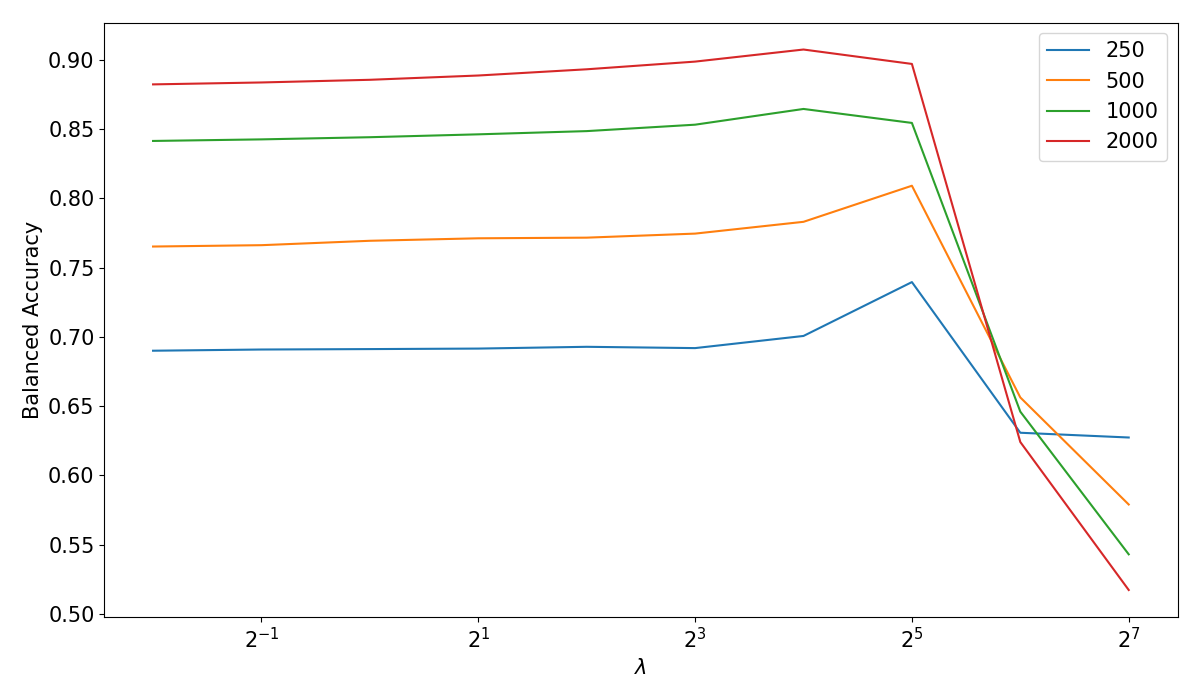
\includegraphics[width=1\textwidth]{analysis/model_convergence/images/jump_penalties.png}
    \caption{Hyper-tuning.}
    \label{fig:jump_penalties}
\end{figure}

\begin{figure}[H] 
    \centering
    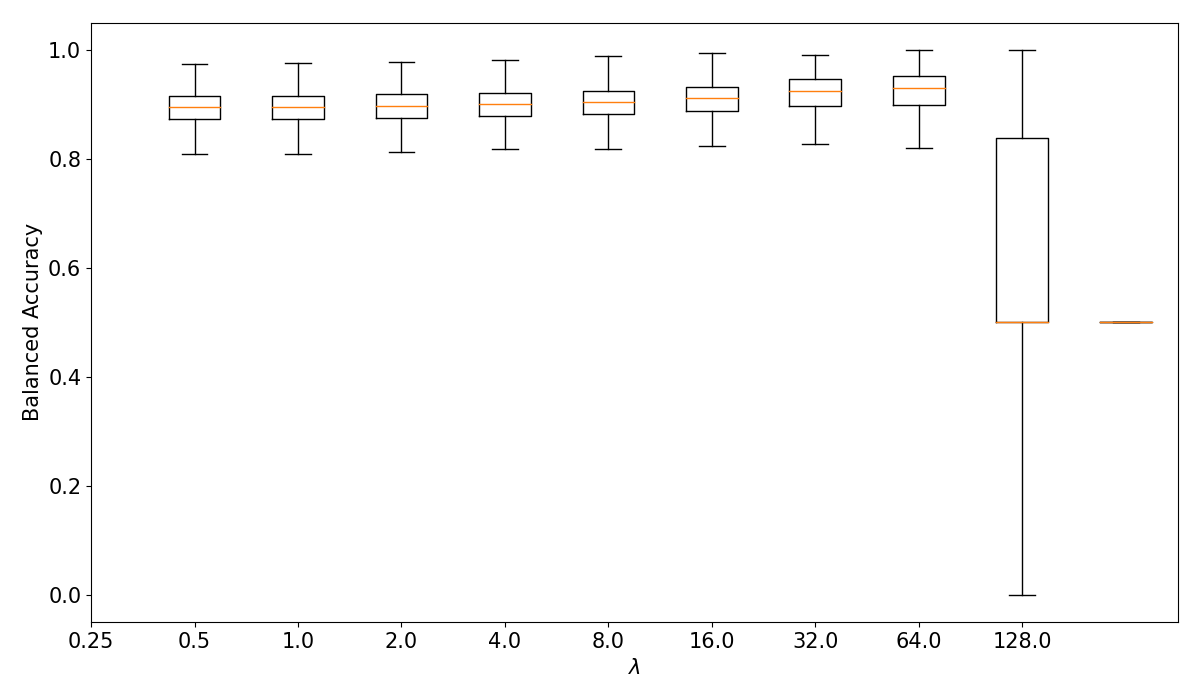
\includegraphics[width=1\textwidth]{analysis/model_convergence/images/jump_penalties_box.png}
    \caption{Hyper-tuning.}
    %\label{fig:jump_penalties}
\end{figure}


\subsection{Simulation study with correctly specified distributions}

\begin{figure}[H] 
    \centering
    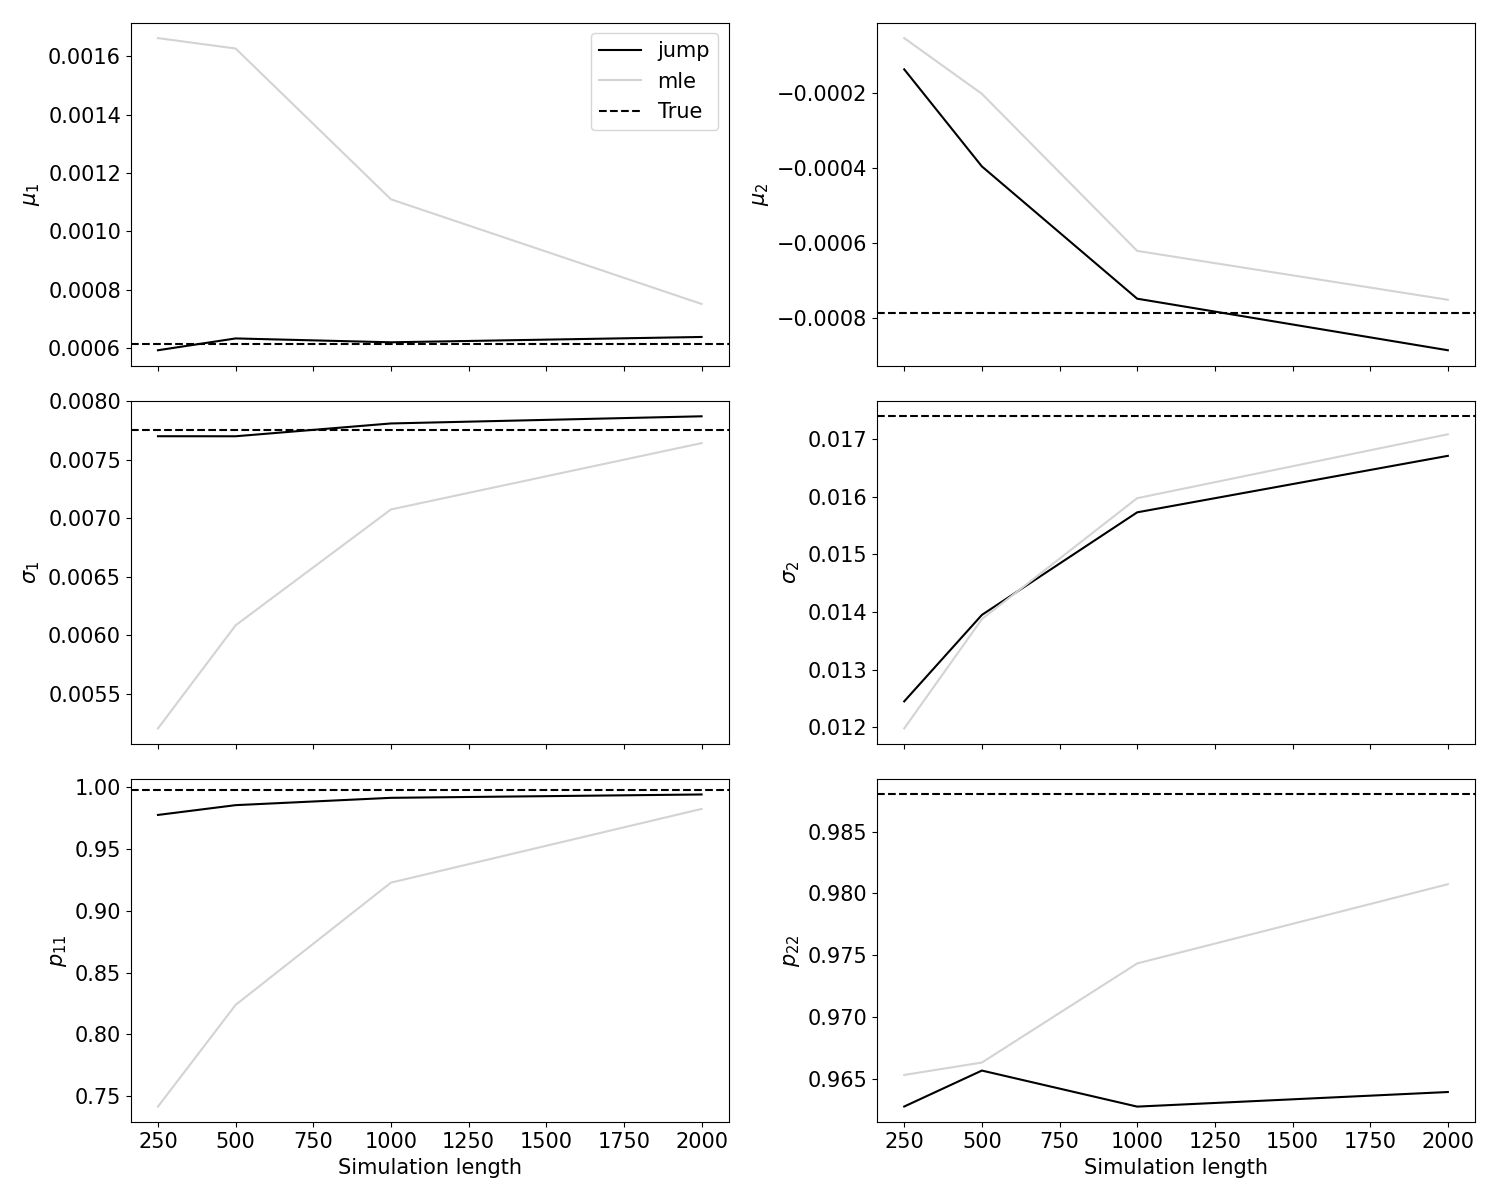
\includegraphics[width=1\textwidth]{analysis/model_convergence/images/simulation_normal.png}
    \caption{Hyper-tuning.}
    %\label{fig:jump_penalties}
\end{figure}

\begin{table}[H]
\centering
\caption{Estimated mean model parameters based on 1000 different simulations from conditional gaussian distributions}
\begin{tabular}{llrrrrrr}
\toprule
     &      &  $\mu_1$ &  $\mu_2$ &  $\sigma_1$ &  $\sigma_2$ &  $q_{11}$ &  $q_{22}$ \\
sample_size & model &          &          &             &             &           &           \\
\midrule
250  & true &   0.0006 &  -0.0008 &      0.0078 &      0.0174 &    0.9979 &    0.9880 \\
     & mle &   0.0017 &  -0.0000 &      0.0052 &      0.0121 &    0.7410 &    0.9658 \\
     & jump &   0.0006 &  -0.0001 &      0.0079 &      0.0113 &    0.9770 &    0.8903 \\
500  & true &   0.0006 &  -0.0008 &      0.0078 &      0.0174 &    0.9979 &    0.9880 \\
     & mle &   0.0015 &  -0.0002 &      0.0060 &      0.0139 &    0.8152 &    0.9719 \\
     & jump &   0.0006 &  -0.0003 &      0.0079 &      0.0130 &    0.9834 &    0.8898 \\
1000 & true &   0.0006 &  -0.0008 &      0.0078 &      0.0174 &    0.9979 &    0.9880 \\
     & mle &   0.0011 &  -0.0006 &      0.0071 &      0.0160 &    0.9208 &    0.9763 \\
     & jump &   0.0006 &  -0.0006 &      0.0080 &      0.0152 &    0.9866 &    0.9420 \\
2000 & true &   0.0006 &  -0.0008 &      0.0078 &      0.0174 &    0.9979 &    0.9880 \\
     & mle &   0.0008 &  -0.0007 &      0.0076 &      0.0171 &    0.9823 &    0.9817 \\
     & jump &   0.0006 &  -0.0007 &      0.0080 &      0.0164 &    0.9951 &    0.9679 \\
\bottomrule
\end{tabular}

\end{table}

 
\subsection{Simulation study with misspecified distributions}

\begin{figure}[H] 
    \centering
    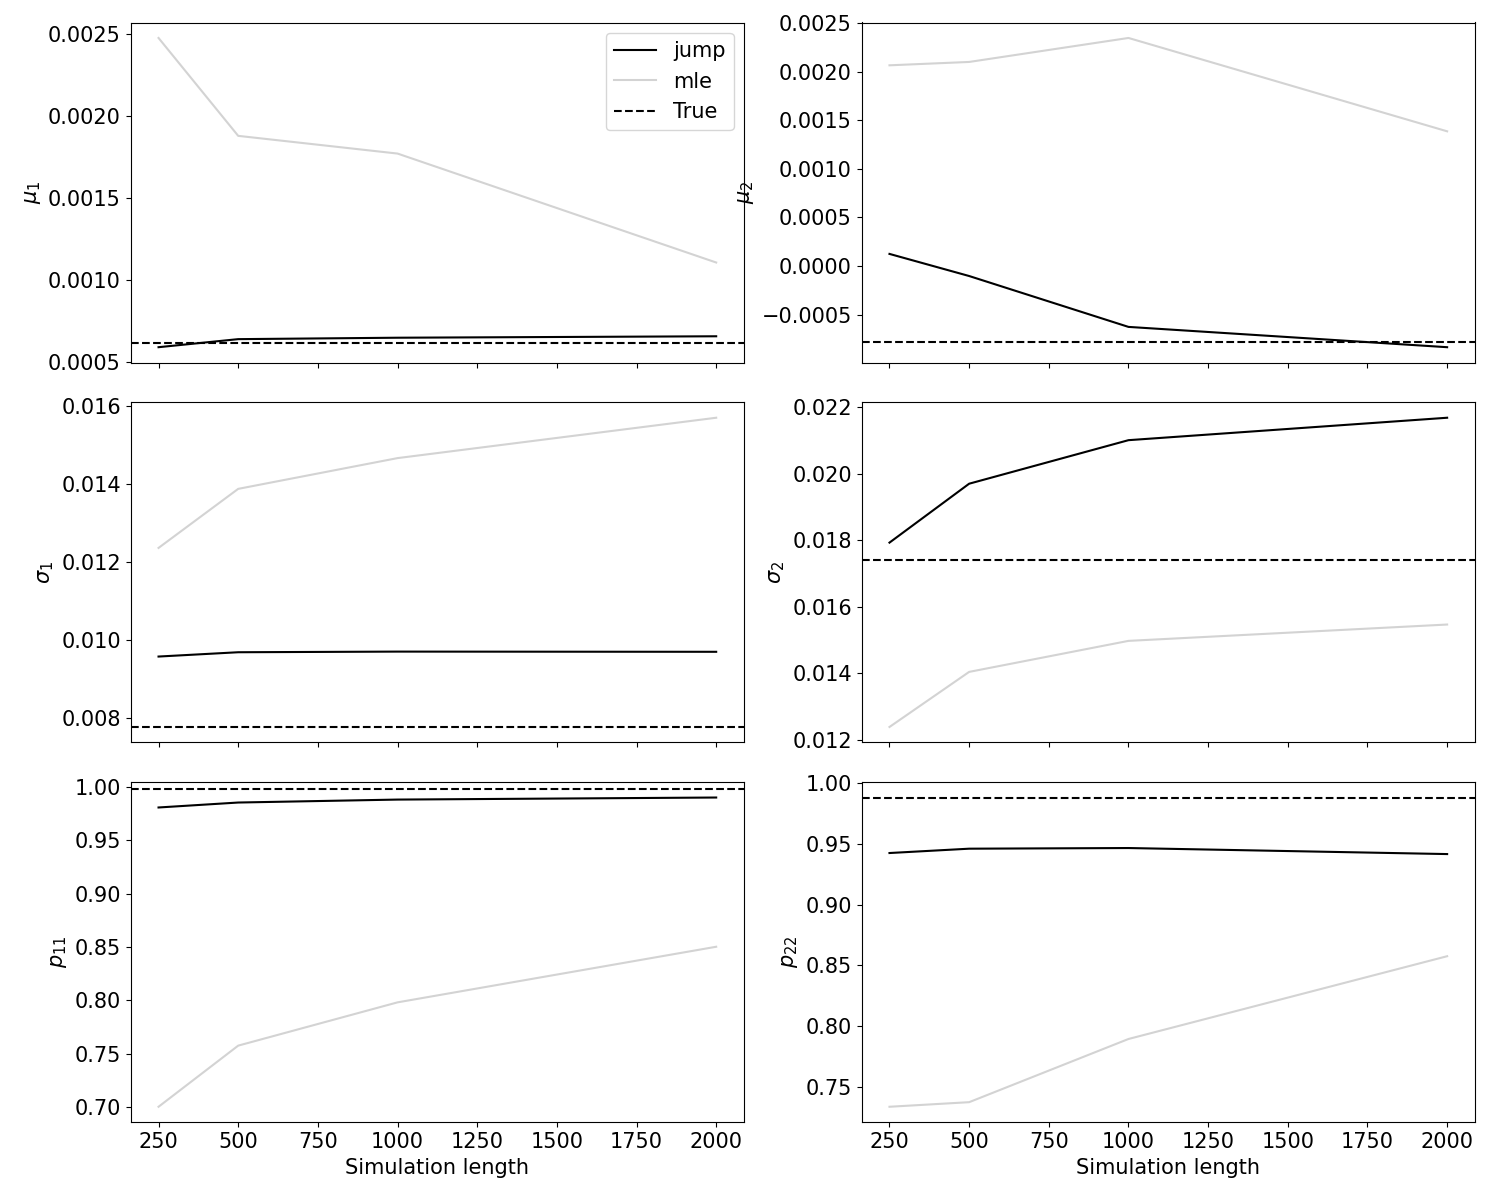
\includegraphics[width=1\textwidth]{analysis/model_convergence/images/simulation_t.png}
    \caption{Estimated mean model parameters based on 1000 different simulations from conditional t-distributions with five degrees of freedom}
    %\label{fig:jump_penalties}
\end{figure}

\begin{table}[H]
\centering
\caption{Estimated mean model parameters based on 1000 different simulations from conditional t-distributions}
\begin{tabular}{llrrrrrr}
\toprule
     &      &   $\mu_1$ &   $\mu_2$ &  $\sigma_1$ &  $\sigma_2$ &    $q_11$ &    $q_22$ \\
sample_size & model &           &           &             &             &           &           \\
\midrule
250  & true &  0.000615 & -0.000785 &    0.007759 &    0.017397 &  0.997900 &  0.988000 \\
     & mle &  0.002475 &  0.002068 &    0.012354 &    0.012383 &  0.700296 &  0.733797 \\
     & jump &  0.000591 &  0.000125 &    0.009567 &    0.017927 &  0.980719 &  0.942377 \\
500  & true &  0.000615 & -0.000785 &    0.007759 &    0.017397 &  0.997900 &  0.988000 \\
     & mle &  0.001878 &  0.002102 &    0.013870 &    0.014039 &  0.757573 &  0.737563 \\
     & jump &  0.000640 & -0.000103 &    0.009677 &    0.019699 &  0.985360 &  0.945942 \\
1000 & true &  0.000615 & -0.000785 &    0.007759 &    0.017397 &  0.997900 &  0.988000 \\
     & mle &  0.001769 &  0.002351 &    0.014671 &    0.014961 &  0.797976 &  0.789653 \\
     & jump &  0.000648 & -0.000627 &    0.009694 &    0.021009 &  0.988130 &  0.946477 \\
2000 & true &  0.000615 & -0.000785 &    0.007759 &    0.017397 &  0.997900 &  0.988000 \\
     & mle &  0.001107 &  0.001388 &    0.015695 &    0.015464 &  0.850219 &  0.857551 \\
     & jump &  0.000657 & -0.000836 &    0.009689 &    0.021683 &  0.990051 &  0.941516 \\
\bottomrule
\end{tabular}

\end{table}
    \section{Model estimation and selection}

\newpage
\section{Data}
\label{section: Data}
In this chapter, the data used to uncover the economic regimes are introduced. A variety of different index will be described, however, the application of them will be specified in subsequent analysis. Initially, decisions related to time horizon and optimal observation frequencies are discussed along with a assessment of which financial data that best captures changing regimes. Once the index data has been introduced and reviewed its distributional and temporal properties are explored in section \ref{subsection: distributional properties} and \ref{subsection: temporal properties}. The objective of the chapter is thus to provide an overview of the data that serves as potential usage for regime detection along with its statistical properties. It should be noted that other indices could have been included, hence the chapter is not intended to be collectively exhaustive. 

\subsection{Time horizon and frequency of data}
\label{subsection: Data frequency}
When utilising financial market data to uncover economic regime changes, a natural questions arises in terms of which data frequency to use. As described, the objective of DAA is to rebalance the portfolios once a regime shifts has occurred, hence if the regime detection relies on too infrequent data, there is a high probability that several regime shifts will remain hidden. As such, data frequencies longer than a month is not considered. Furthermore, as previously mentioned, macroeconomic data is widely available, thereby contributing to its popularity, however, the data is typically characterised by a data frequency of months or even quarters. Therefore, the data frequency of macroeconomic variables propose a challenge, as historic events has shown that economic regime changes can happen swiftly, evident by the recent COVID-19 recession. As such, monthly data compared to e.g. daily data, greatly increases the risk of slow and insufficient detection of economic regime shifts.
 
Despite of the reasoning just outlined, it should be noted that the use of daily data presents some challenges as well. This is due to the fact that daily returns contain a lot of noise and extreme observations, which are evened out on a monthly basis. Consequently, long-horizon returns tend to be more closely approximated by a Gaussian distribution than returns for short-horizon (Campbell et al. 1997). As such, short-term data frequencies complicates the modeling significantly, which can lead to sporadic predictions and less persistence. In addition, the use of daily return frequencies makes the aforementioned link to macroeconomic data more difficult to justify, and therefore it becomes challenging, from a macroeconomic perspective, to argue that economic regime shifts occur since there is no tangible macroeconomic evidence to support this before the data gets collected and released. Despite of the complications associated with short-term data frequencies, the arguments for considering daily as opposed to monthly data frequencies are compelling. 

Furthermore, despite the aforementioned issues with sporadic predictions due to daily data frequencies, Bulla et al. (2011) argued that by relying on daily data it becomes feasible to apply filters that increase confidence whenever a regime change has been detected. As such, research cements the possible of implementing a waiting scheme, in which the portfolio manager would wait several days, when a regime shifts has been detected, before changing the portfolio allocation, thereby minimizing the risk of re-allocating capital based on a wrong signal. In addition, the use of MPC makes daily data frequencies more justified, since it is not possible to make better return predictions for the assets than their long-term average. As such, looking only a limited number of days into the future is not just an approximation necessary to make the optimization problem computationally feasible, it is also reasonable due to the nature of financial returns.

Bulla et al. (2011) further argued that the use of daily data frequencies increases the amount of data available for markets characterised by a short lifetime, however, many financial indices are old and for these older indices monthly data is more available than daily data. Unsupervised machine learning models, such as HMMs, require large amounts of data to be trained in order to achieve a desired and comfortable level of predictability, and as such, the usage of these heavy data-driven models serve as an argument for relying on monthly data as opposed to daily data. Yet, this thesis favors early detection, due to the reasoning outlined above. As a result, daily data, will be used in the analysis. Lastly, the optimal time horizon used for training the model is debatable, however, it should at least span the time required for a financial cycle to unfold in order to include the performance of DAA strategies in several economic environments. Furthermore, it should be acknowledged that, the longer the data horizon the more questionable it becomes whether stationarity of the data-generating process can be assumed (Bulla et al. 2011).

The following sections will include details on selected indices used for training the hidden Markov models, in order to uncover whether different indices lead to similar model parameters and performance across DAA strategies. 

\subsection{The MSCI}
\label{subsection: MSCI Index}
The MSCI World Index captures large and mid cap representation across 23 Developmed Markets (DM) countries. As such, the difference compared to the well-known MSCI ACWI Index is the exclusive weight on assets from developed economies. With 1,600 constituents, the index covers approximately 85\% of the free-float-adjusted market captilization in each country. The weights across country and sectors are shown in figure XXXXY as of November 2020. The historical development of the index is depicted in figure \ref{fig:MSCI_index}. 
 
\begin{figure}[H] 
    \centering
    
\includegraphics[width=1.0\textwidth]{analysis/data_description/images/MSCI_index.png}
    \caption{Development MSCI.}
    \label{fig:MSCI_index}
\end{figure}

%##### INDSÆT FIGUR AF Sector og region focus ####### # VIS split

The inclusion of the MSCI World Index is based on the fact that it is a global index, and thus should capture the economics trends across geographies. As such, the thesis treats it as a baseline index in terms of uncovering economic-regimes. Although it is a world index, North America makes up almost 2/3 of the index, however, this makes sense from an economic perspective since the U.S. economy serves as a fundamental indicator of how the remaining world economy is progressing. Furthermore, the information technology sector is by far the largest sector in the index, since it accounts for approximately 22\% of the overall allocation as per figure XXXXX. It should be noted that the weights are a snapshot in time, hence they are constantly changing. 

\begin{table}[H]
\caption{Summary statistics for the daily MSCI log-returns.}
\centering
\begin{tabular}{c c c c c c c c c} 
\hline\hline
Observations & Mean & STD & Skewness & Excess Kurtosis & Min & Max & First ACF & Annual SR \\
\hline
12,941 & 0.0003 & 0.0087 & -0.6521 & 10.8819 & -0.1044 & 0.0909 & 0.1337 & 0.4854 \\
\hline
\end{tabular}
\label{tab:summary_stats_MSCI}
\end{table}

Table \ref{tab:summary_stats_MSCI} shows the first four central moments together with the minimum and maximum observation, the first-order autocorrelation and the annual Sharpe ratio (SR). The SR is the excess return per unit risk, i.e. the excess return divided by the standard deviation (SD). The first observations originates from 1969-12-31 and the final included observations is the date 2021-02-12. It appears that the daily log-returns for the MSCI World Index are negatively skewed and the distribution is also characterised by being highly leptokurtic as the excess kurtosis is positive. As such, the summary statistics indicate that the log return series for the MSCI World Index, are characterised by the set of stylized facts that are commonly associated with financial returns. The range of the observations has a span of 0.1953, thereby indicating that the index can change significantly in high-volatility periods.    
 
\subsection{The S\&P 500}
The S\&P 500 is a stock index comprising 500 companies from the U.S. which was founded in 1957. The stocks that make up the index are selected by a committee which include representation from all major segments in American industry. As such, contrary to prevailing public sentiment, the index is not simply made up of the 500 largest companies in the U.S. The S\&P 500 Index is a market-capitalization-weighted index in which the 10 largest companies account for 27.5\% of the capitalization of the index as of per December 2020. Figure \ref{fig: SP500_index} showcases the development of the S\&P 500 Index since origination. 
 
\begin{figure}[H] 
    \centering
    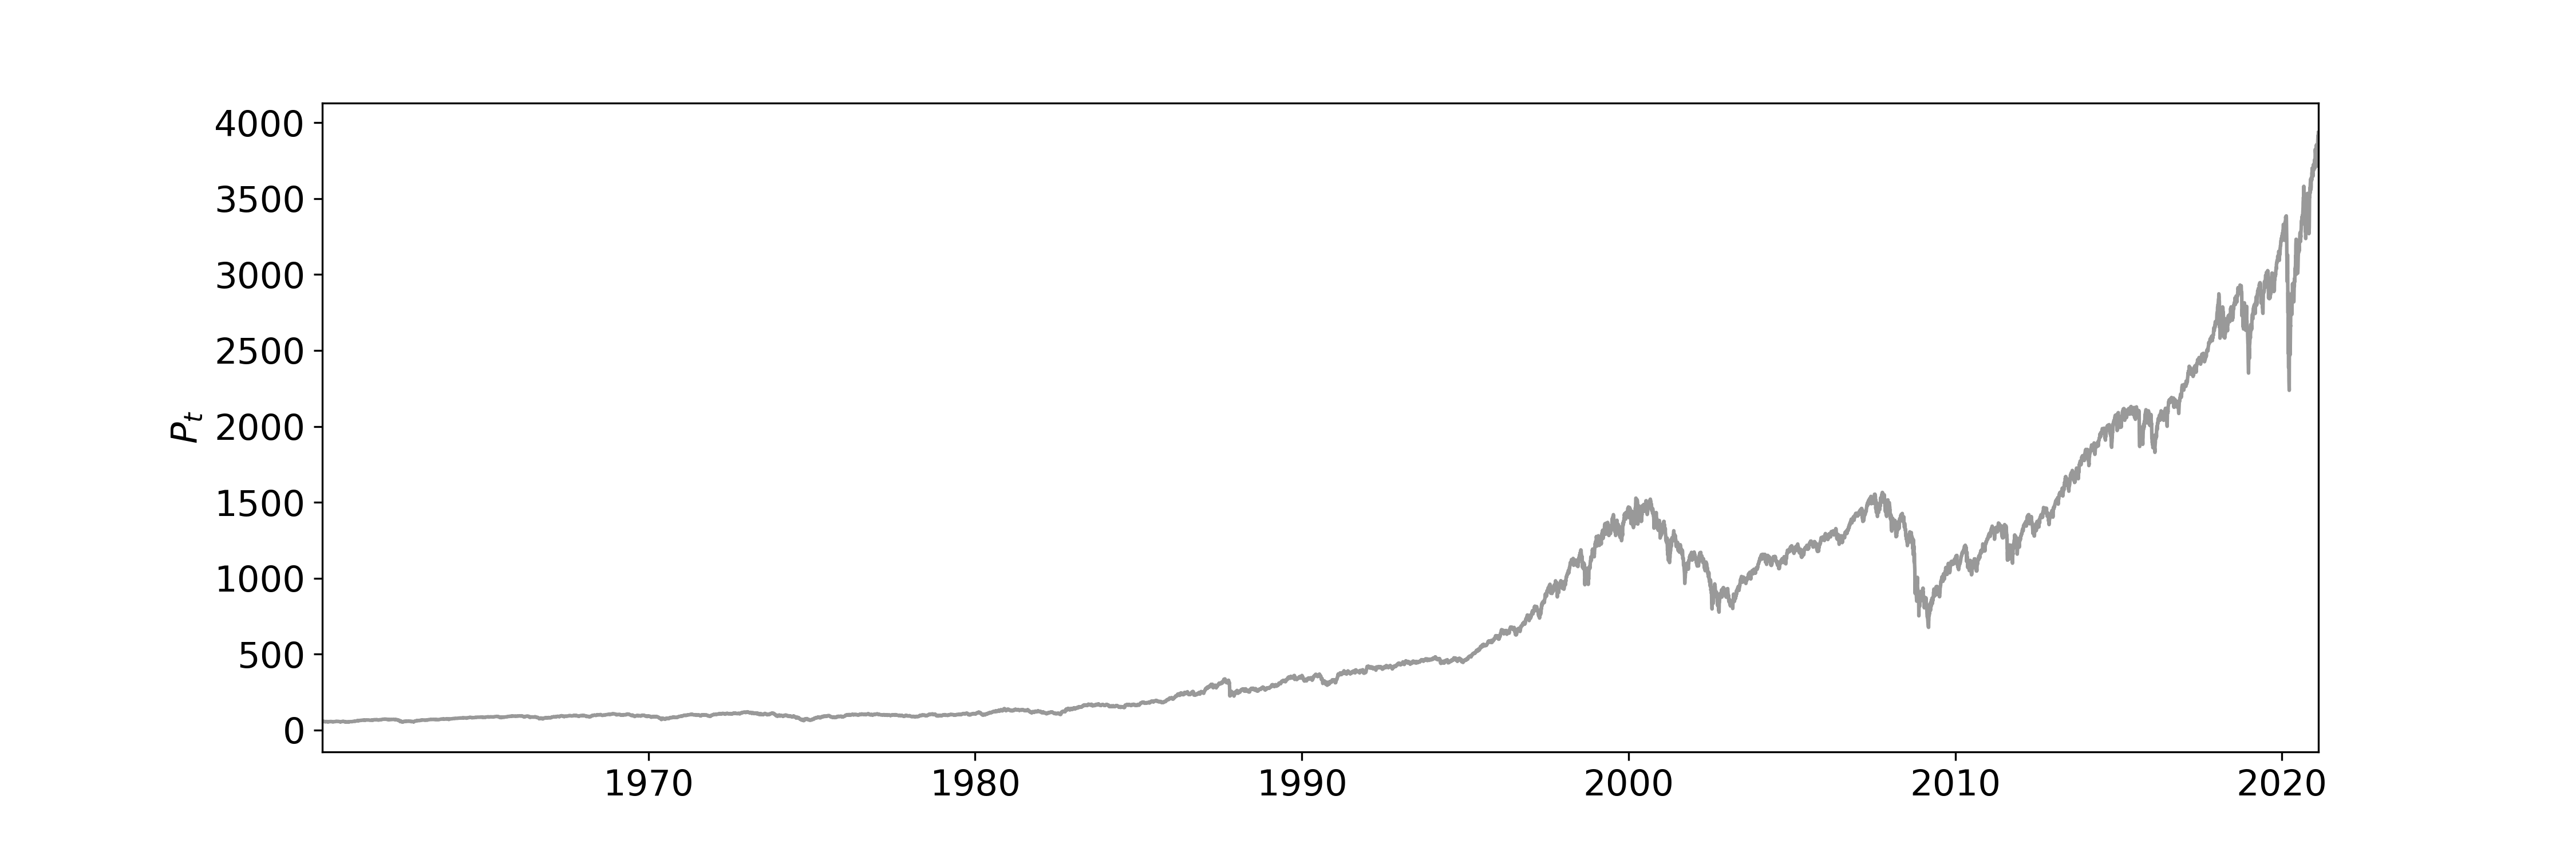
\includegraphics[width=1\textwidth]{analysis/data_description/images/SP500_index.png}
    \caption{Development S\&P 500.}
    \label{fig: SP500_index}
\end{figure}

As is evident from figure \ref{fig: SP500_index} the 44 year data period has been impacted by the major market movements including black monday in 1987 as well as the dot-com bubble of the late 90s and early 2000s. Furthermore the attractive bull market leading up to the GFC has been well-captured by the development of the S\&P 500 Index. Lastly, the long bull market following the GFC as well as the recent COVID-19 correction and rebound appears to be well-captured by the S\&P 500 Index, thereby indicating that it will serve well for model estimation purposes.  

It is unlikely that the recent bullish environment for stocks will continue in perpetuity, since interest rates and inflation, at some point, are likely to start increasing. When that happens, investments towards stocks and indexes can procure short to mid-term monetary losses, however, it is evident from figure \ref{fig: SP500_index} that there appears to be a strong upwards trend historically, thus supporting the argument for capital allocation towards stocks in general.


\begin{table}[H]
\caption{Summary statistics for the daily S\&P 500 log-returns.}
\centering
\begin{tabular}{c c c c c c c c c} 
\hline\hline
Observations & Mean & STD & Skewness & Excess Kurtosis & Min & Max & First ACF & Annual SR \\
\hline
15,385 & 0.0003 & 0.0103 & -1.0353 & 23.8338 & -0.2290 & 0.1096 & -0.006 & 0.4350 \\
\hline
\end{tabular}
\label{tab:summary_stats_S&P500}
\end{table}
 
Compared to the MSCI Index it is evident by table \ref{tab:summary_stats_S&P500} that the daily log-returns of the S\&P 500 encompass similar mean daily returns, although the daily standard deviation is higher. Furthermore, the S\&P 500 Index is more left-skewed, more leptokurtic and the range is much larger at 0.3386. The larger range can primarily be attributed to the black monday event of 1987 in which the S\&P 500 was much harder impacted relative to the other included indexes. Naturally, these conclusions leads to a lower annual Sharpe Ratio of 0.4350 compared to the MSCI which holds an annual Sharpe Ratio of 0.4854.
 
\subsection{DAX 30}
\label{subsection: DAX 30}
The DAX is a blue chip stock market index comprising the 30 largest listed German companies. It is similar in nature to FTSE 100 and the Dow Jones Industrial Average. The index is included in the analysis in order to get an estimate for, whether the model parameters will change significantly when trained on the DAX as opposed to the aforementioned indexes. As such, the DAX becomes particularly interesting since its composition of a small number of firms and a restrictive geographical focus on Germany means that it might not necessarily represent the vitality of the economy as a whole. 

\begin{figure}[H] 
    \centering
    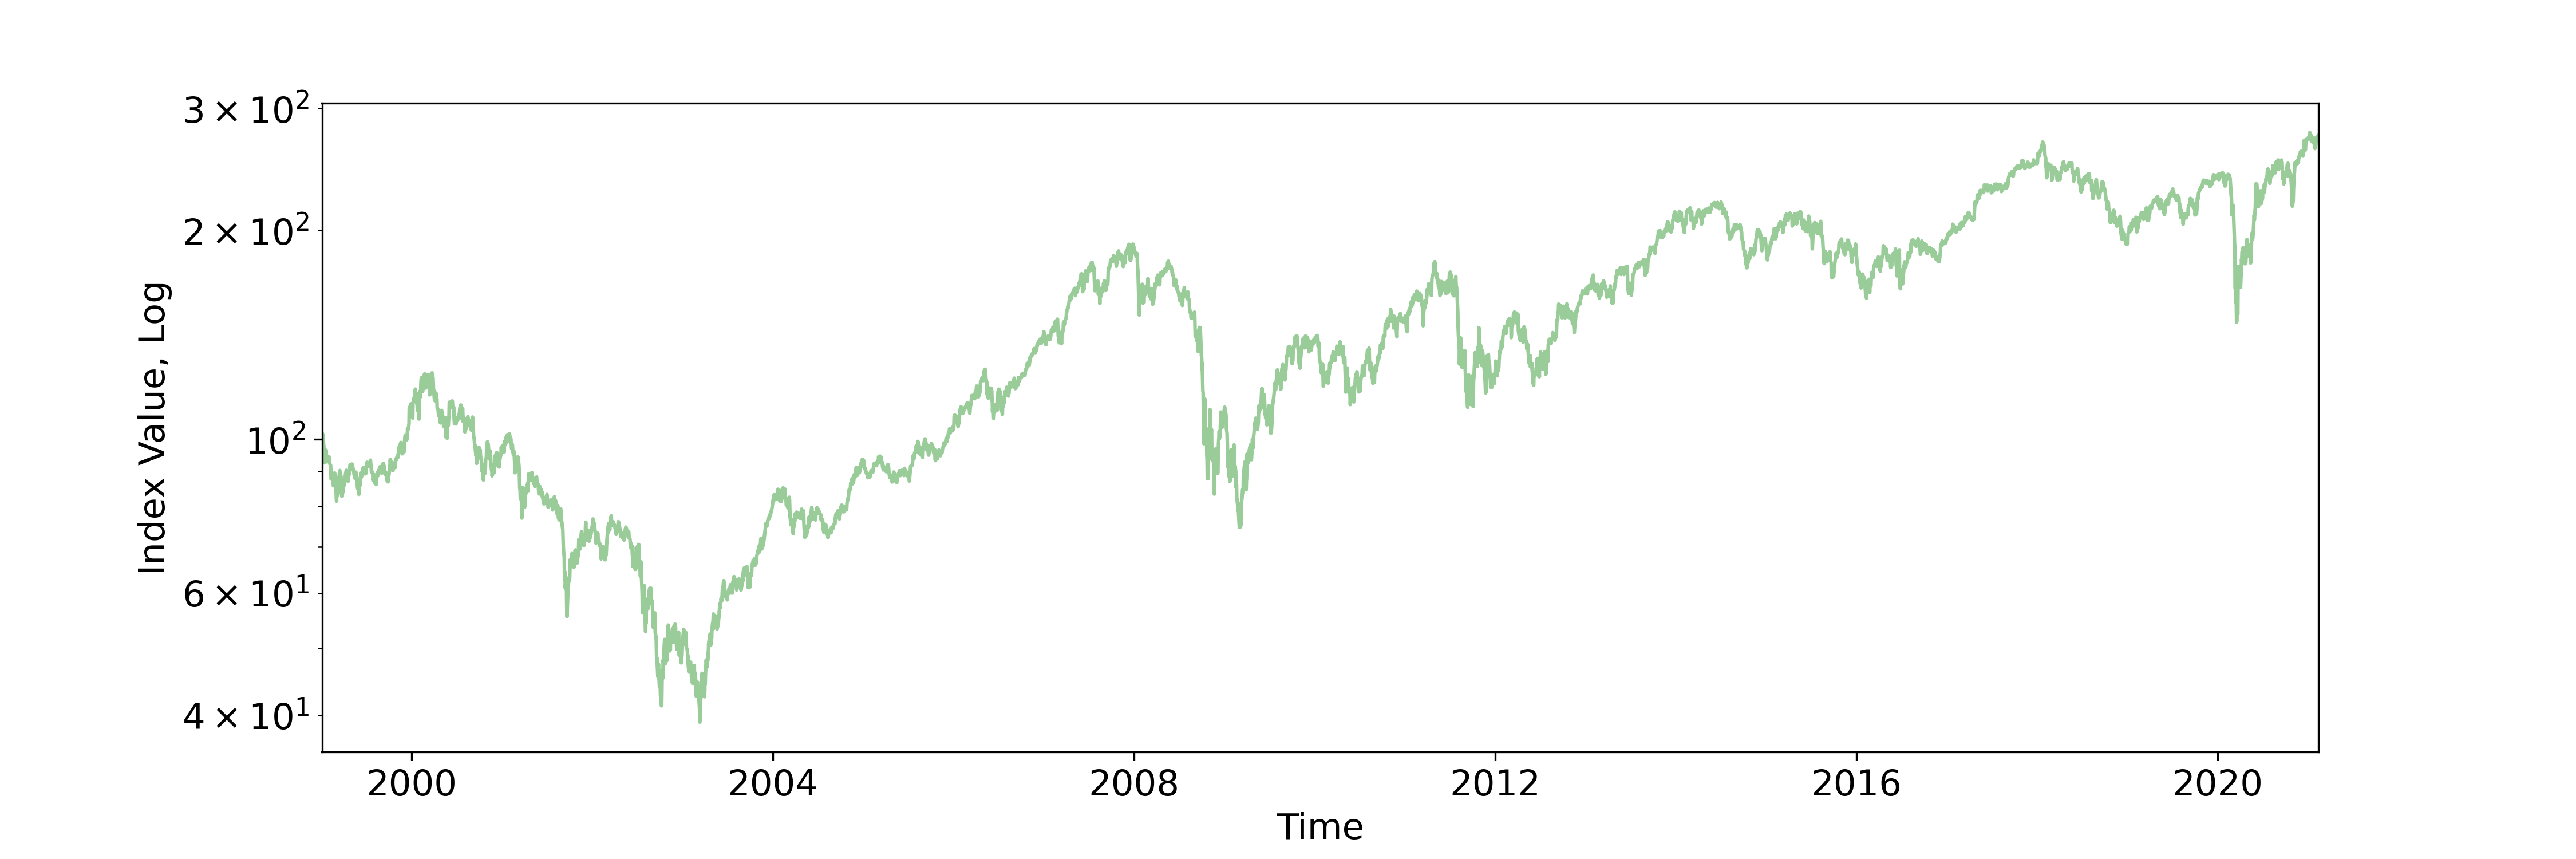
\includegraphics[width=1\textwidth]{analysis/data_description/images/DAX_index.png}
    \caption{Development DAX 30.}
    \label{fig: DAX_index}
\end{figure}

As is evident by figure \ref{fig: DAX_index}, the availability of daily data is significantly shorter compared to the MSCI World and the S\&P 500 Index. This is primarily due to the fact that the DAX 30 was originated in the late 1987. However, figure \ref{fig: DAX_index} also showcases that recent financial bear markets such as the dot-com bubble of the early 2000s, the GFC of 2008 as well as the COVID-19 rebound in Q1/Q2 2020 are well captured by DAX 30 Index. 

Since January 2006, the index is refreshed every second, however, the thesis will continue to rely on daily data frequencies as discussed in section \ref{subsection: Data frequency}. The index is capitalization-weighted and holds a total market capitalization of 1,017.7 billion EUR as of 21st of September 2020. In response to the recent accounting scandal related to Wirecard, Deutshce Börse announced an expansion of the DAX 30 to include 40 members. The expansion is set to occur in the third quarter of 2021.

\begin{table}[H]
\caption{Summary statistics for the daily DAX log-returns.}
\centering
\begin{tabular}{c c c c c c c c c} 
\hline\hline
Observations & Mean & STD & Skewness & Excess Kurtosis & Min & Max & First ACF & Annual SR \\
\hline
5,613 & 0.0002 & 0.0159 & -0.1869 & 2.8115 & -0.1394 & 0.1257 & 0.0146 & 0.1839 \\
\hline
\end{tabular}
\label{tab:summary_stats_DAX}
\end{table}

As highlighted by table \ref{tab:summary_stats_DAX}, the DAX Index contains much fewer observations compared to the MSCI World and S\&P 500 index. Furthermore, the DAX has similar mean daily returns although the standard deviation is the highest among the selected indices. However, the DAX is less negatively skewed and exhibit the lowest degree of leptokurtotic among the selected indexes. However, the high standard deviation naturally leads to a much lower Sharpe Ratio compared to the other indices at 0.1839.

\subsection{Distributional properties}
An overview of the development for the three selected indexes have been plotted in figure \ref{fig: all_indices_index}, however, the indexes have been adjusted so that they all comprise the same amount of observations. This means that the first observation is from 04-01-1999 and the last observation is 12-02-2021. 
\begin{figure}[H] 
    \centering
    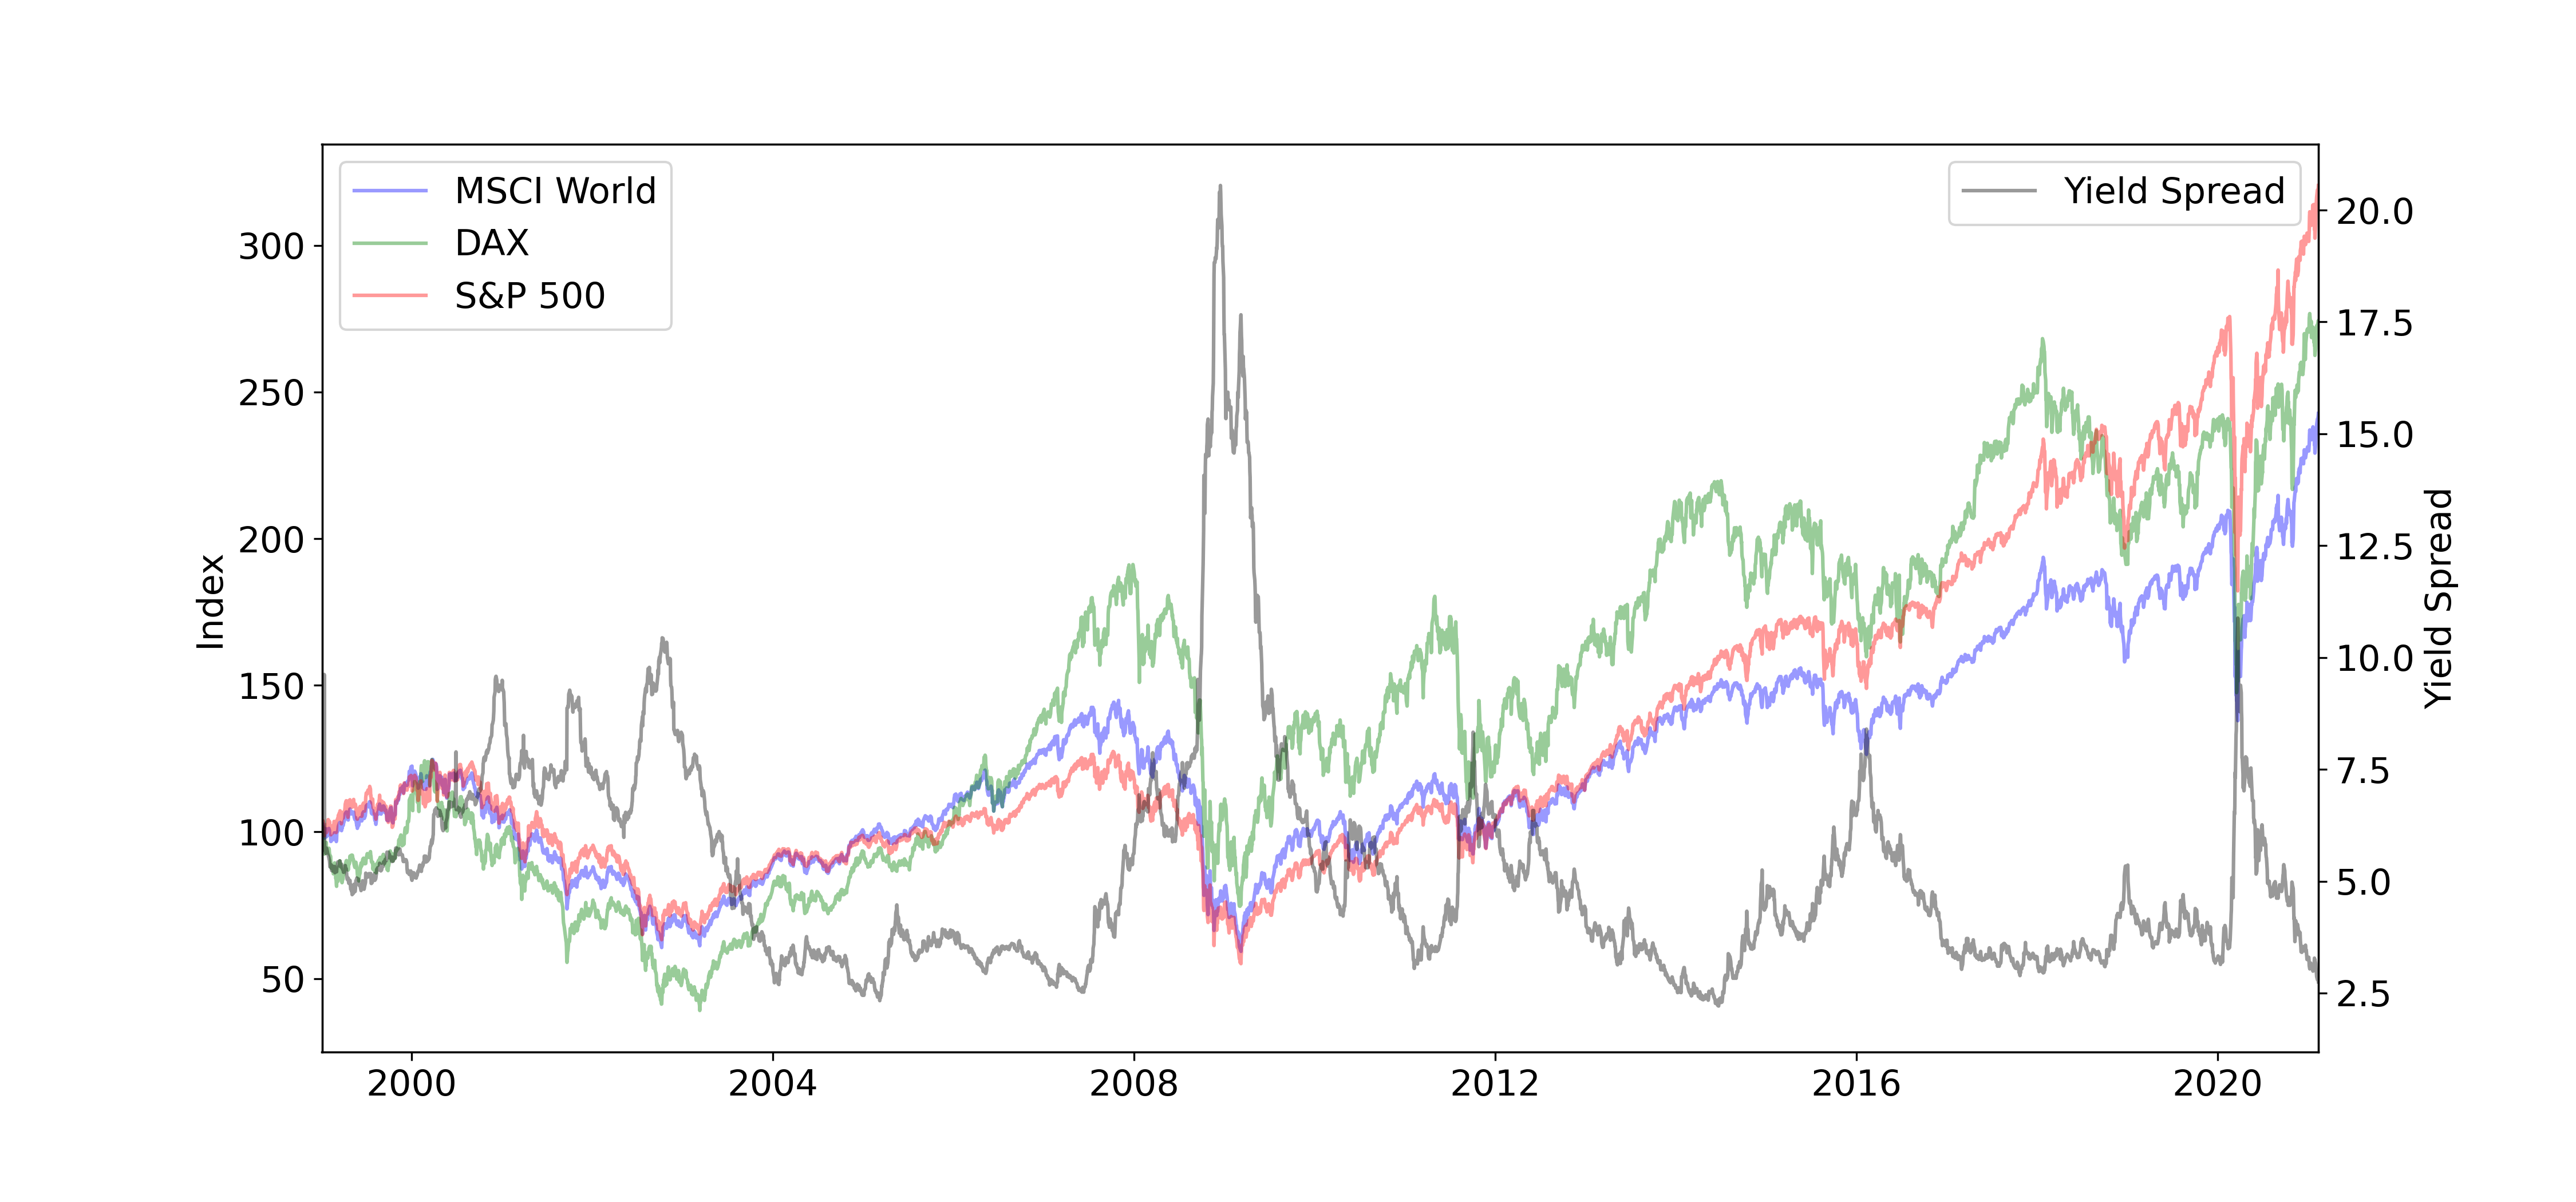
\includegraphics[width=1.0\textwidth]{analysis/data_description/images/comb_index.png}
    \caption{Development all indices.}
    \label{fig: all_indices_index}
\end{figure}

From an overall return perspective it is evident that the S\&P 500 Index has performed better than the other alternatives. Interestingly, the S\&P 500 Index only recovered from the dot-com bubble a few months prior to the financial crisis of 2008, yet it was severely impacted by the GFC. In the period following the financial crisis the S\&P 500 has been performing increasingly well resulting in an upward-trajectory until the recent COVID-19 correction, after-which the index reached the present all time high values. 

The MSCI World Index appears to have a more stable trajectory with less volatile movements both compared to the S\&P 500 and the DAX 30. Despite this, the MSCI World Index generally trended in the same direction as the S\&P 500,
but in some periods the range between the two indices widened. For example,
it appears that the MSCI World and S\&P 500 Index trended in close correlation in the period from 1999 to 2015, however, from 2015 to 2021 the two indices have drifted apart. Furthermore, it appears that the S\&P 500 has become increasingly more volatile over the period 2015-2021, particularly evident by the recent COVID-19 rebound in which the drawdown of the S\&P 500 was much more extreme compared to the MSCI World.  

The DAX 30 performed particularly well in the period following the dot-com bubble, however, during 2008 and 2009 the GFC severely impacted the index, thereby bringing it down to the respective levels of the S\&P 500 and MSCI World. As concluded in section \ref{subsection: DAX 30} the DAX was characterised as the most volatile, which is also evident by figure \ref{fig: all_indices_index} which showcases that the DAX indeed appears to have a higher volatility. From 2006 to 2017 the DAX Index has consistently been at higher index levels compared to the other indices until the S\&P 500 caught up by breaking its all time high in 2019. An overview of the summary statistics for each index is listed in table \ref{tab:summary_all}.

\begin{table}[H]
\caption{Summary statistics for the daily log-returns of the three indices}
\centering
\begin{tabular}{c c c c}
\hline
 & MSCI World & S\&P 500 & DAX 30 \\
\hline 
Observations & 12,941 & 15,385 & 5,613 \cr Mean & 0.0003 & 0.0003 & 0.0002 \cr STD & 0.0087 & 0.0103 & 0.0159 \cr Skewness & -0.6521 & -1.0353 & -0.1869 \cr Excess Kurtosis & 10.8819 & 23.8338 & 2.8115 \cr Min & -0.1044 & -0.2290  & -0.1394 \cr Max & 0.0909 & 0.1096 & 0.1257 \cr Annual SR & 0.4854 & 0.4350 & 0.1839
\\
\hline
\end{tabular}
\label{tab:summary_all}
\end{table}

\subsubsection{Log Returns}
As evident by\Cref{fig: all_indices_index} the series are not stationary since the mean values are growing and when zooming in on local periods, the development of the respective index appears to be characterised by strong trends. As such, a transformation is needed to obtain stationary time-series. In cases where the series is characterised by growing means and local trends a log-transformation will narrow the gap between the indices and taking the first difference will eliminate the growing mean values. This results in the log-returns being derived as $r_t = log(P_t) - log(P_{t-1})$, where $P_t$ is the adjusted closing price of the index on day $t$ and $\log$ is the natural logarithm. For daily returns less than 10\%, log returns are a good approximation to the discrete return, as it is the first order Taylor approximation (Nystrup, 2014).

Table \ref{tab:summary_all} showcases the summary statistics for the daily log-returns of the selected indices together with the annual Sharpe ratio and the Jarque-Bera (JB) test statistic. As already noted the distributions are left skewed and strongly leptokurtic, however, this is not a surprising finding given previous studies conducted by Cont (2001) as well as Granger \& Ding (1995b), in which the stylized facts of financial returns were explored substantially. The critical value for the Jarque–Bera test statistic at a 99.9\% significance level is 14.13, in which table \ref{tab:summary_all} clearly highlights that the Jarque–Bera test strongly rejects the normal distribution for all three indices.  

In addition, it is evident from the plot of the kernel density functions in figure ref til figur (de billeder med normalfordeling vs. empirisk fordeling) that the log returns series are characterised by excess kurtosis relative to a Gaussian distribution. As such, there is too much mass centered around the mean and in the tails compared to the Gaussian distribution. The fat left tail implies that using a Gaussian distribution to model returns will underestimate the frequency and magnitude of downside events (Nystrup, 2014). 

\begin{figure}[H] 
    \centering
    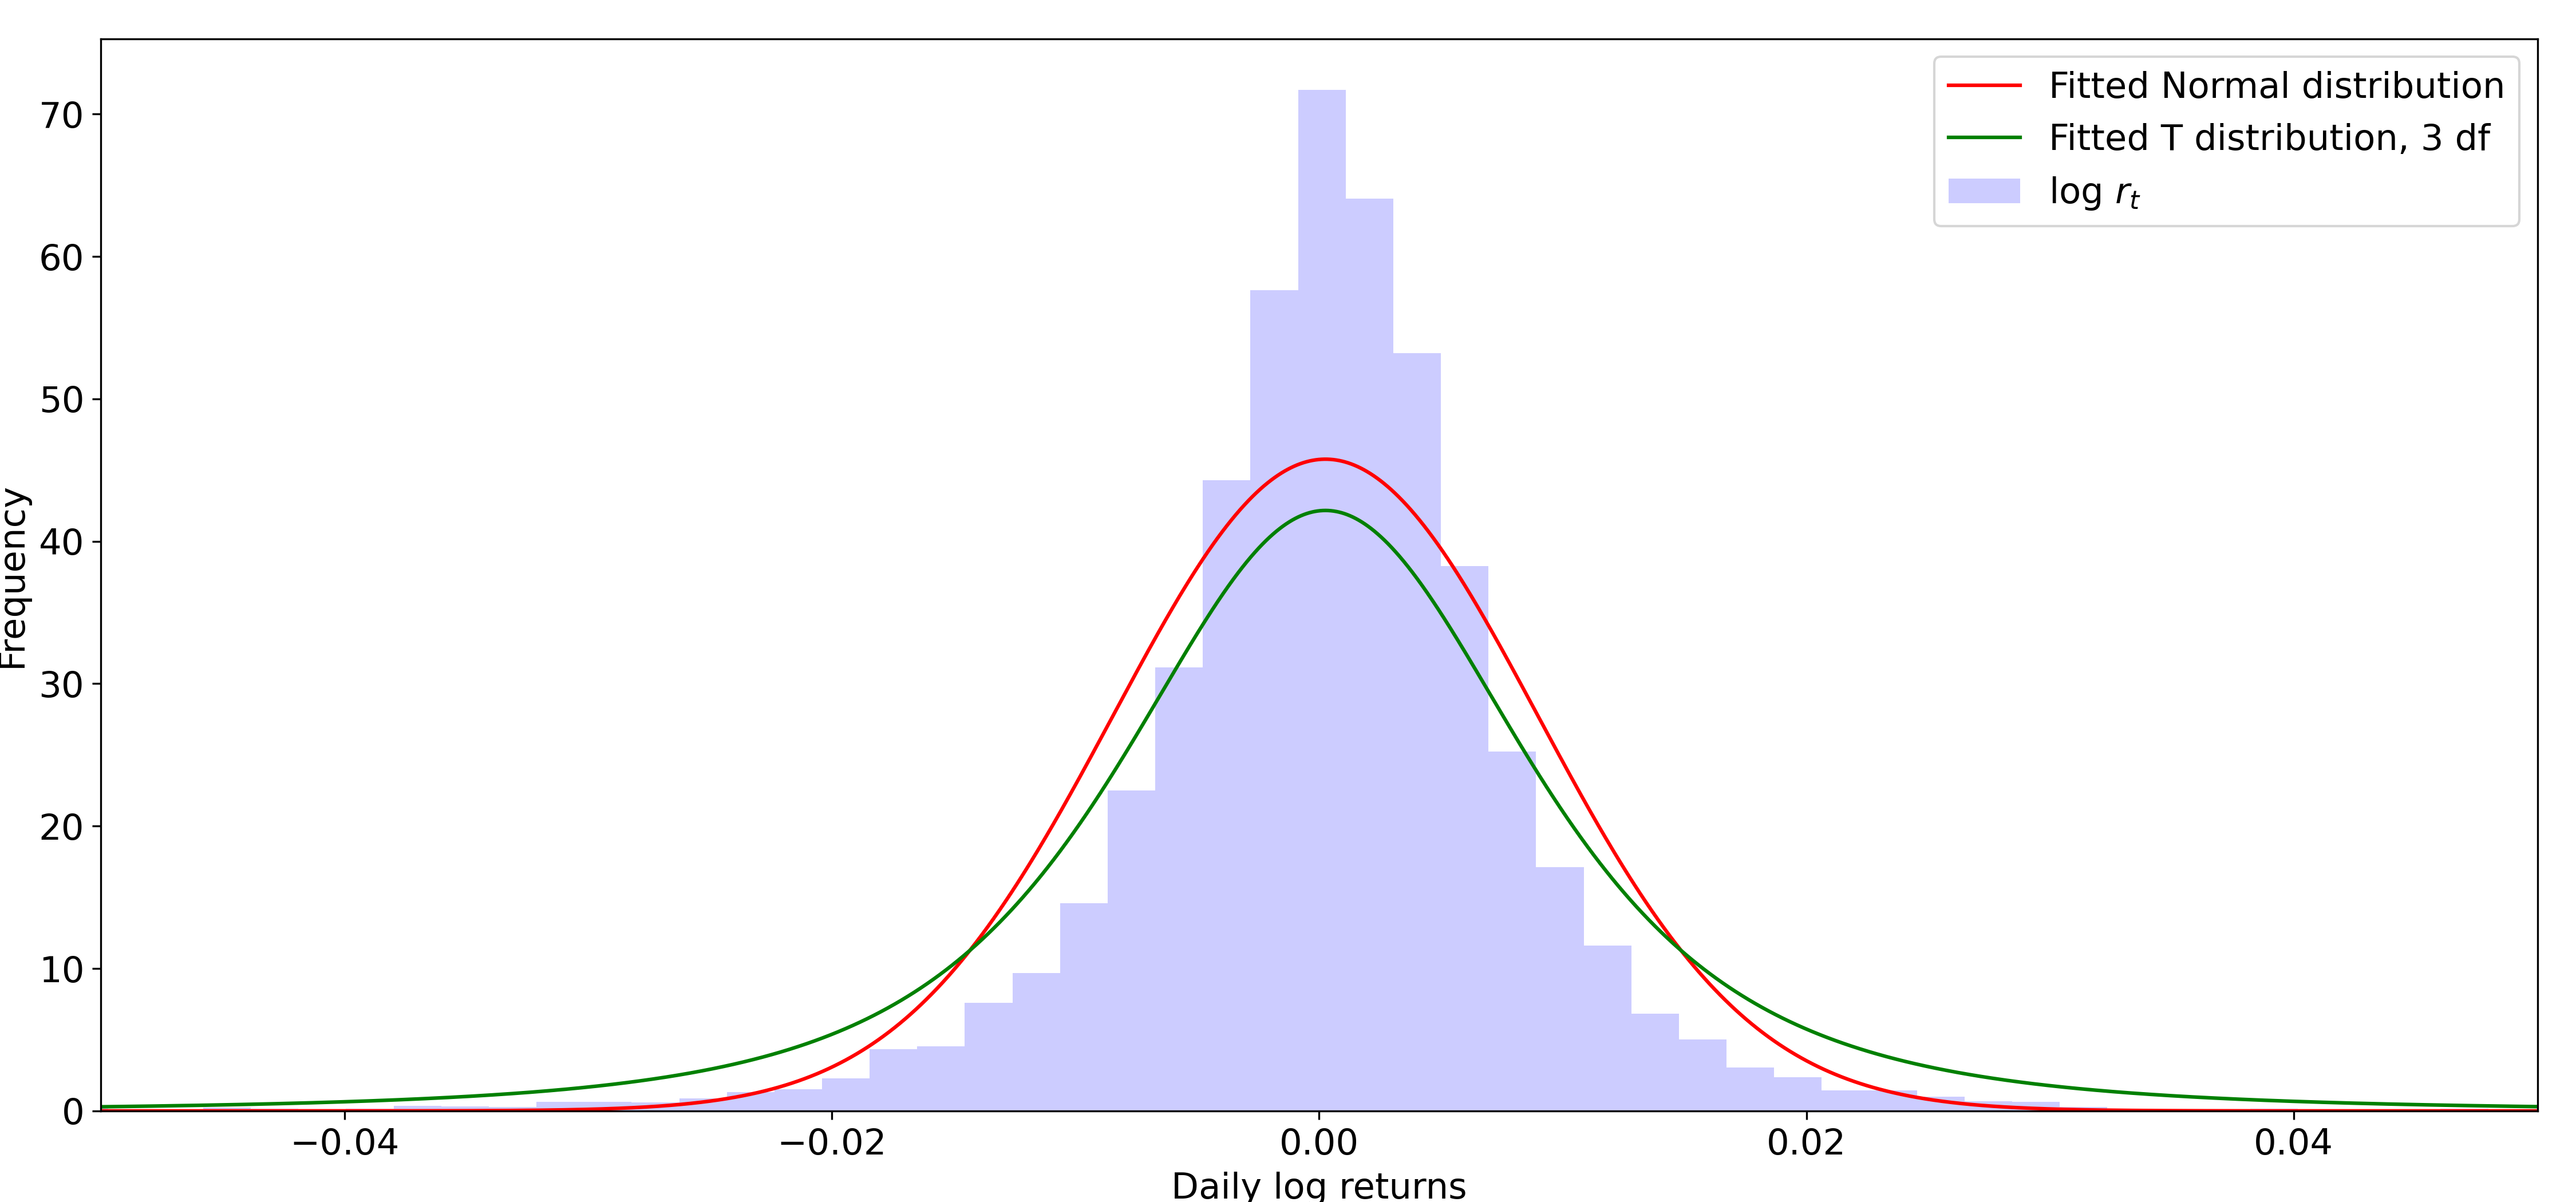
\includegraphics[width=0.65\textwidth]{analysis/data_description/images/MSCI_distribution.png}
    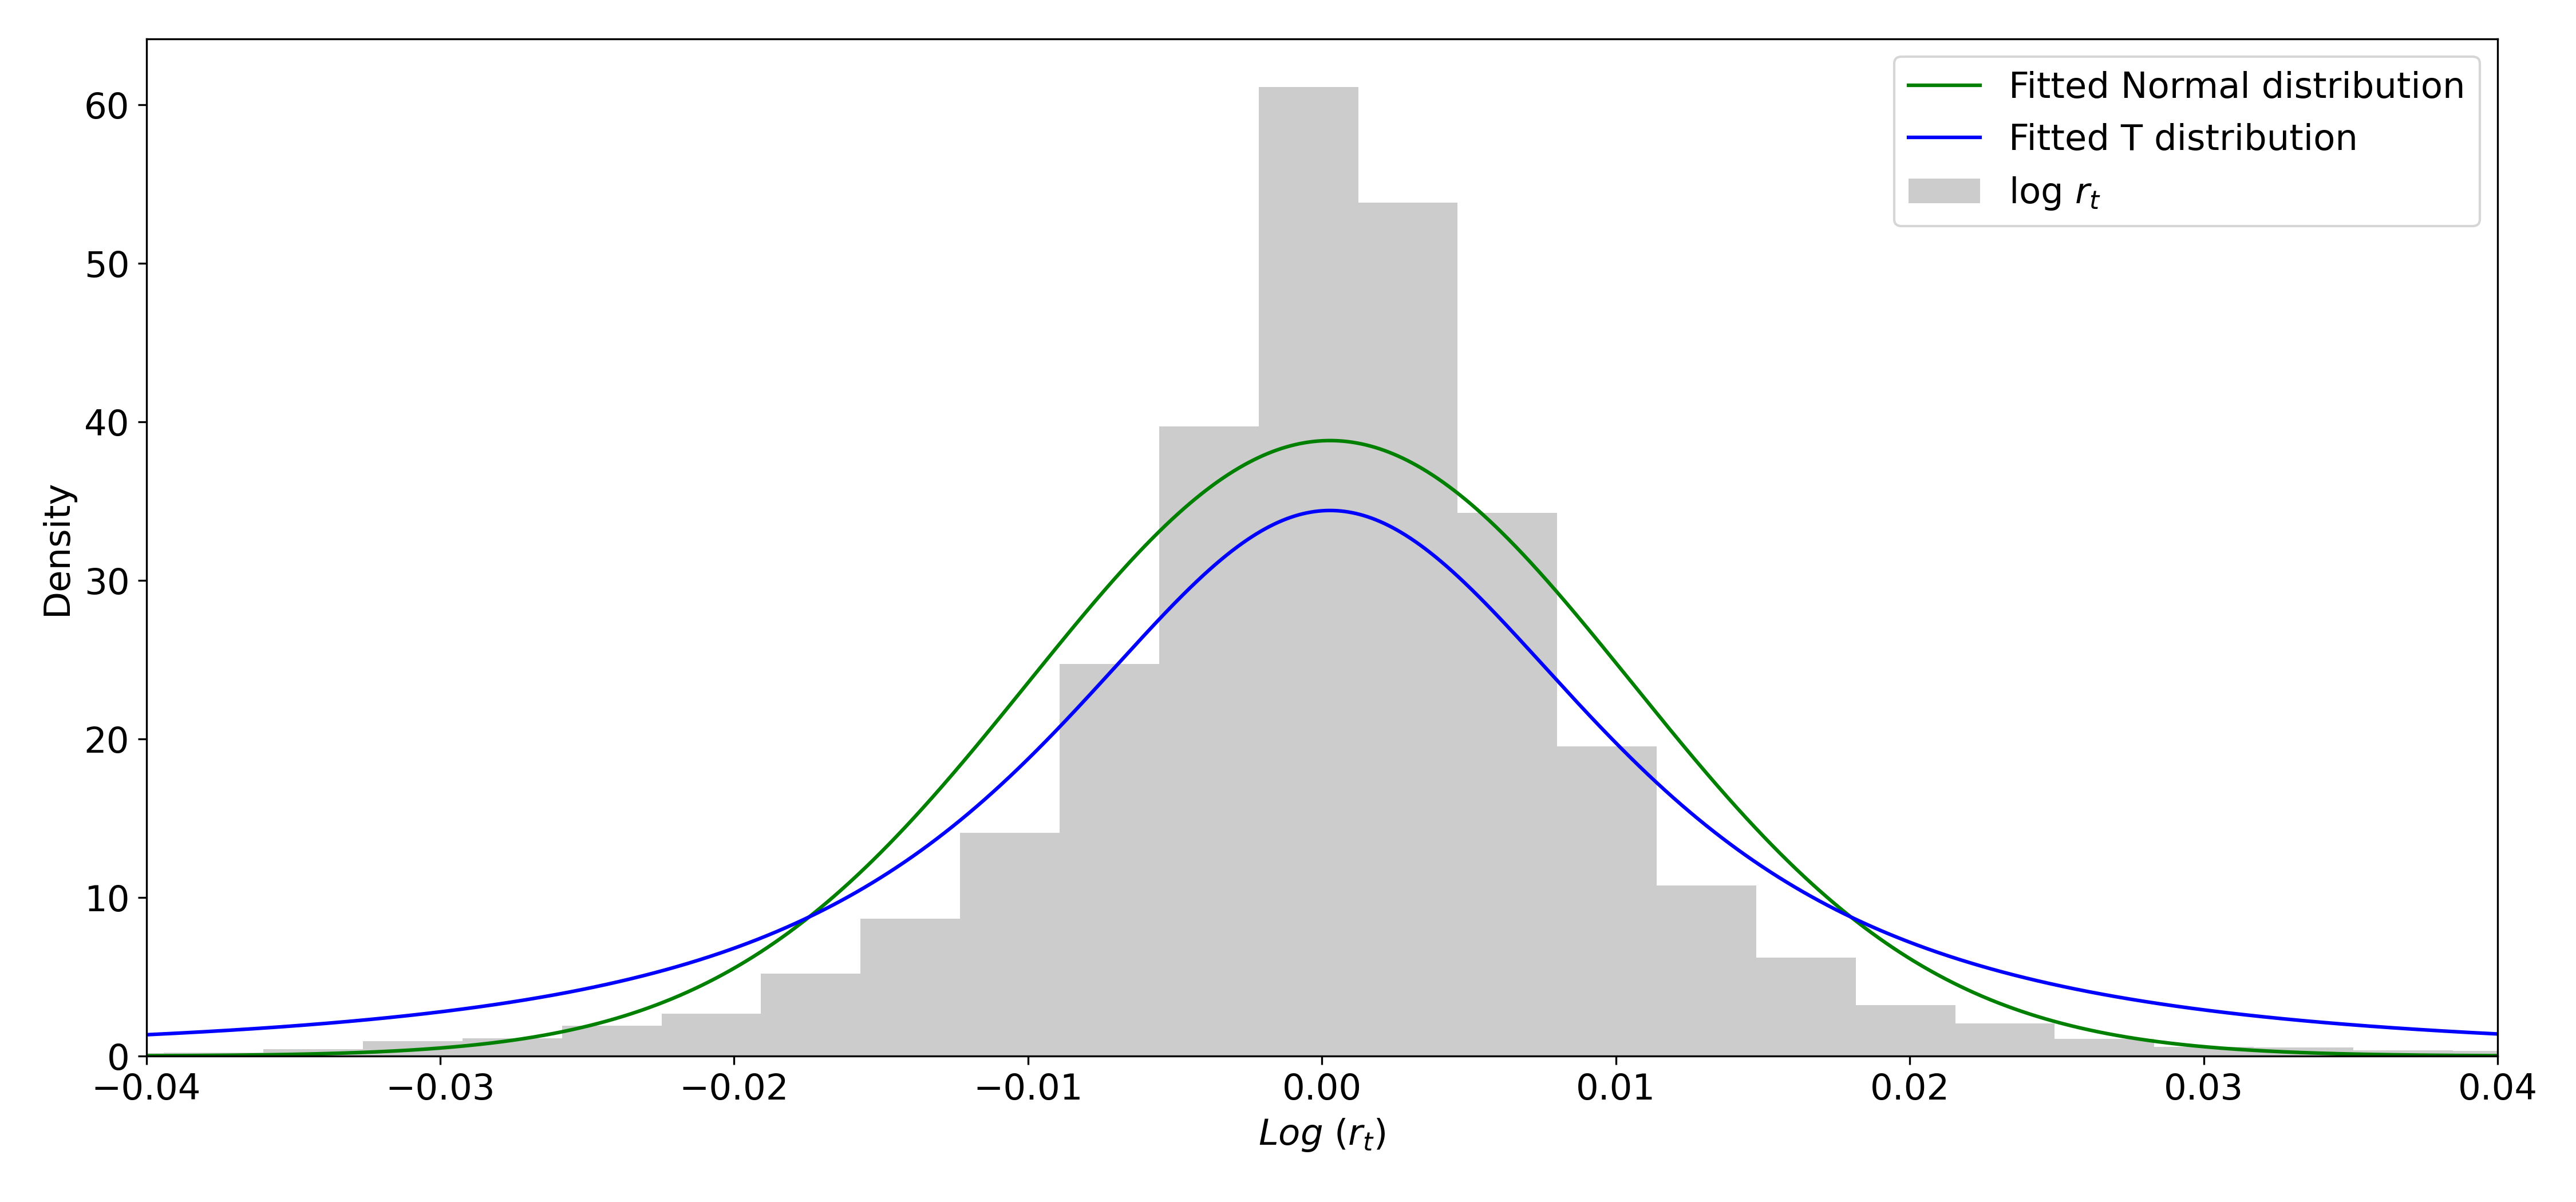
\includegraphics[width=0.65\textwidth]{analysis/data_description/images/SP500_distribution.png}
    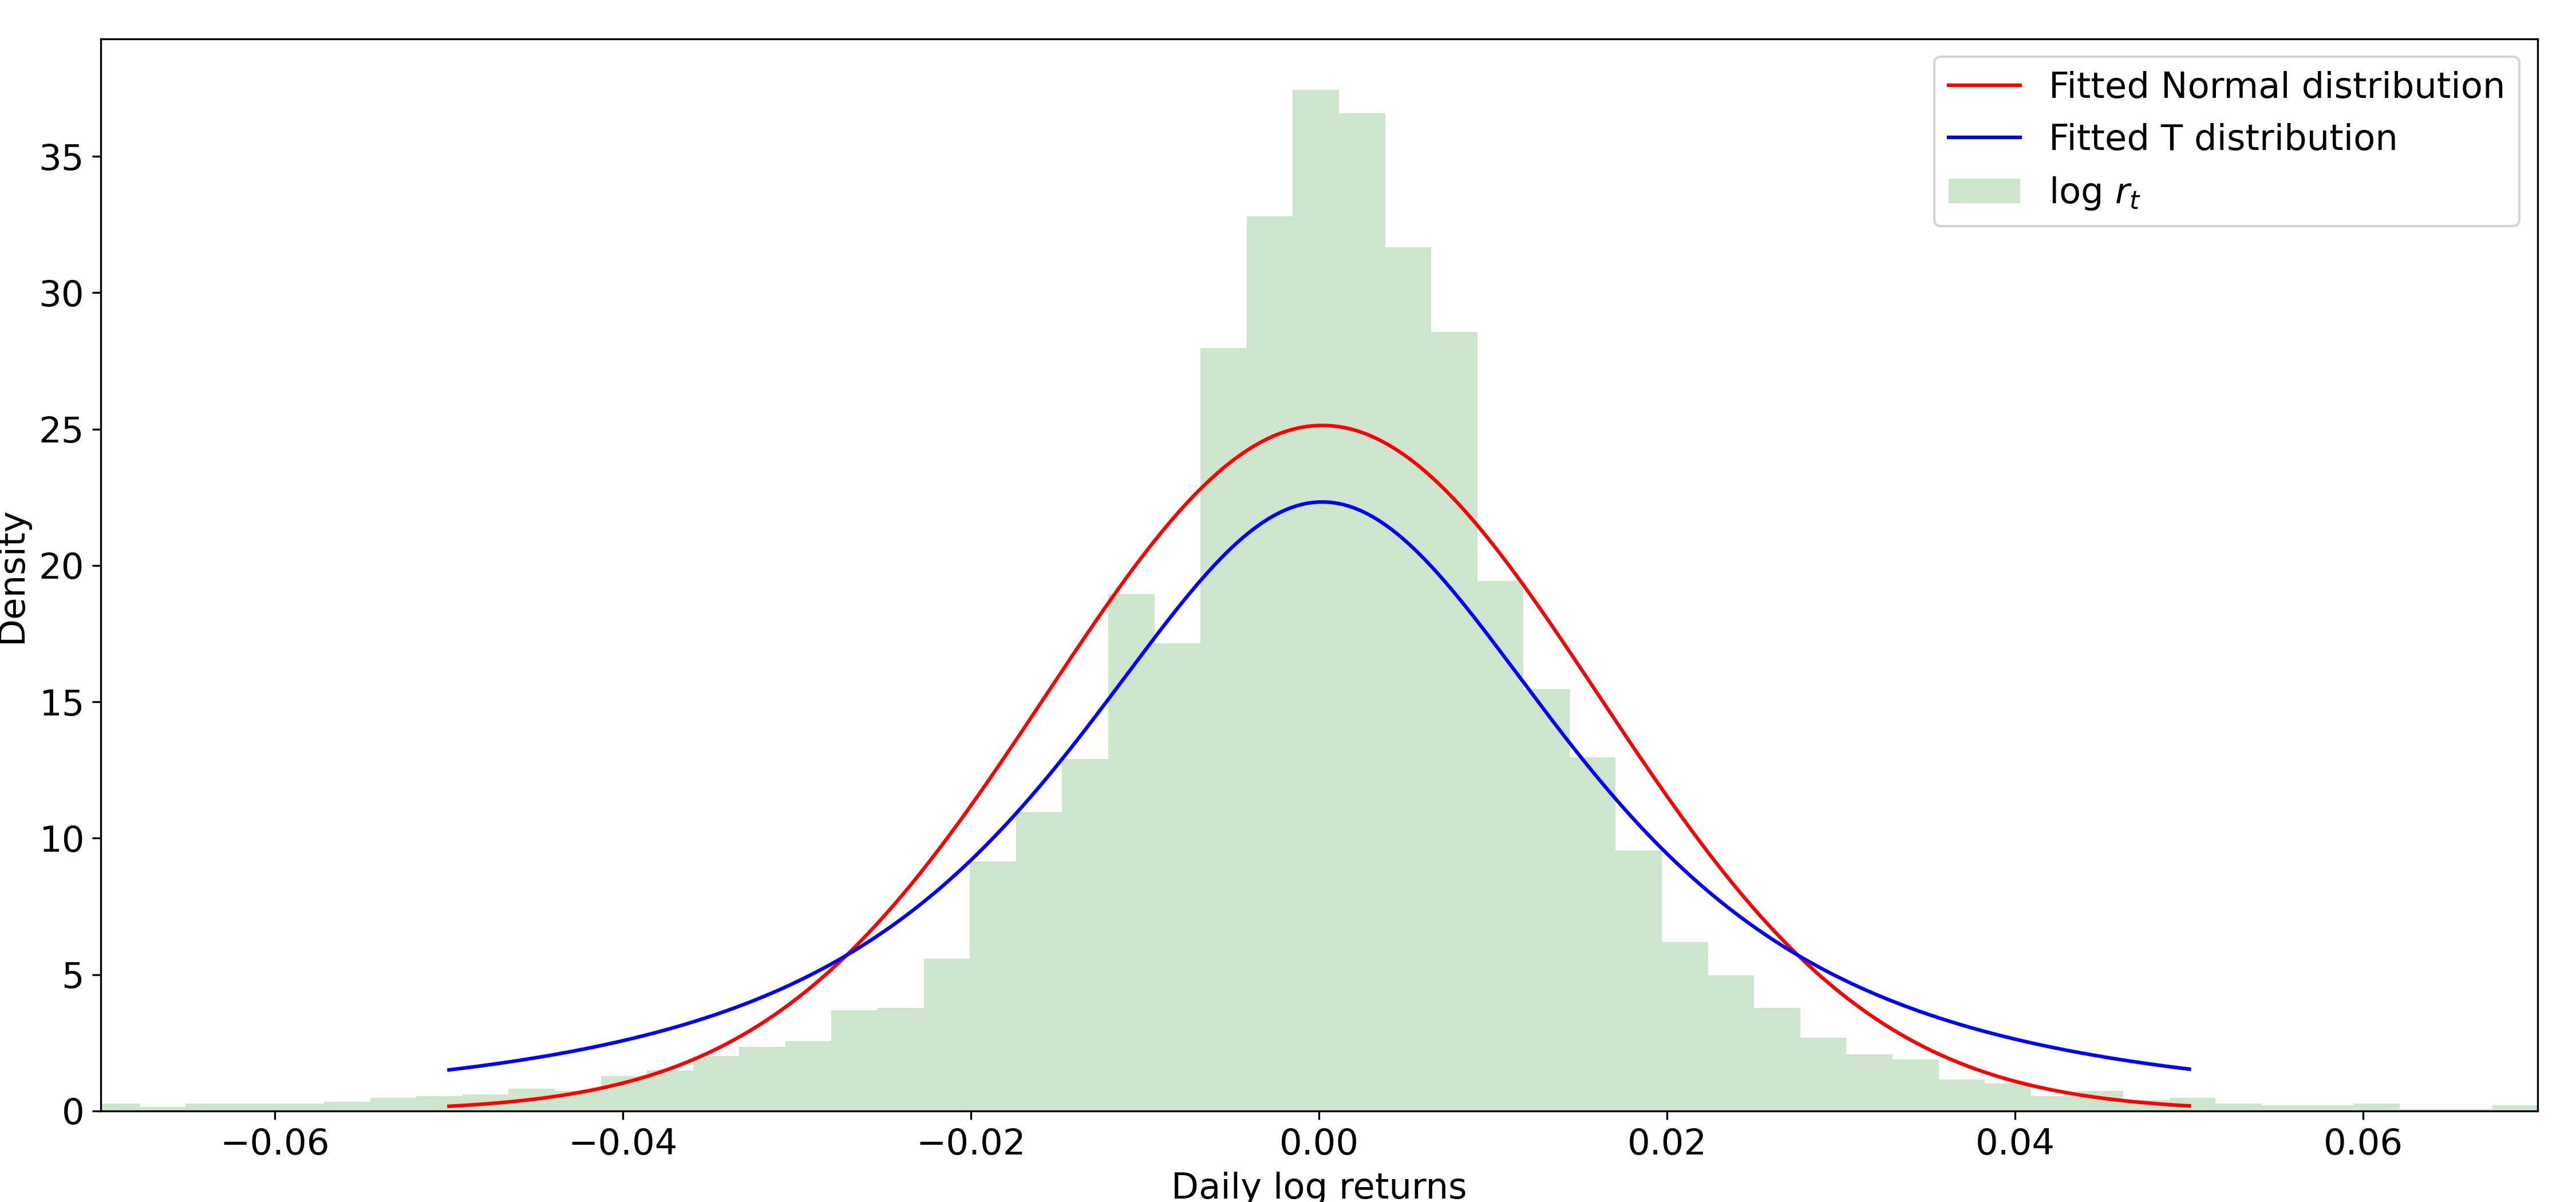
\includegraphics[width=0.65\textwidth]{analysis/data_description/images/DAX_distribution.png}
    \caption{Distributions. MSCI, S\&P500 and DAX respectively.}
    \label{fig: Kernel_distributions}
\end{figure}

Furthermore, it is evident from figure \ref{fig: Kernel_distributions} that all three indices encompass extreme observations that lie more than 3 standard deviations from the mean. There are 187 observations that deviate more than 3 standard deviations from the mean for the MSCI World index which is way above the expected 39 if the series followed a Gaussian distribution. Out of these, 74 observations are located in the right side of the tail while the remaining 113 are located in the left tail. This phenomenon that large drawdowns occur more often than similar large upwards movements is well researched and known as the gain/loss asymmetry (Cont, 2001). In addition, it should be noted that since the MSCI World contains 12,941 observations, it only takes a few outliers to reject that the series follow a normal distribution. However, as noted by Cont (2001), financial returns are characterised by a large degree of extreme observations compared to the Gaussian distribution, which is evident by the large excess kurtosis from table \ref{tab:summary_all}.

Lastly, it is important to note the subtle distingshion between outliers and extreme observations since extreme observations deviate considerably from the group mean, yet they may still hold meaningful information hence they should not be disregarded.
Since extreme events happen in live markets the observation that they create should be included in the model estimation in order for the model be as realistic as possible. As such, a plot of the log returns for all the indices have been constructed in figure \ref{fig: log_returns_all_indices}

\begin{figure}[H] 
    \centering
    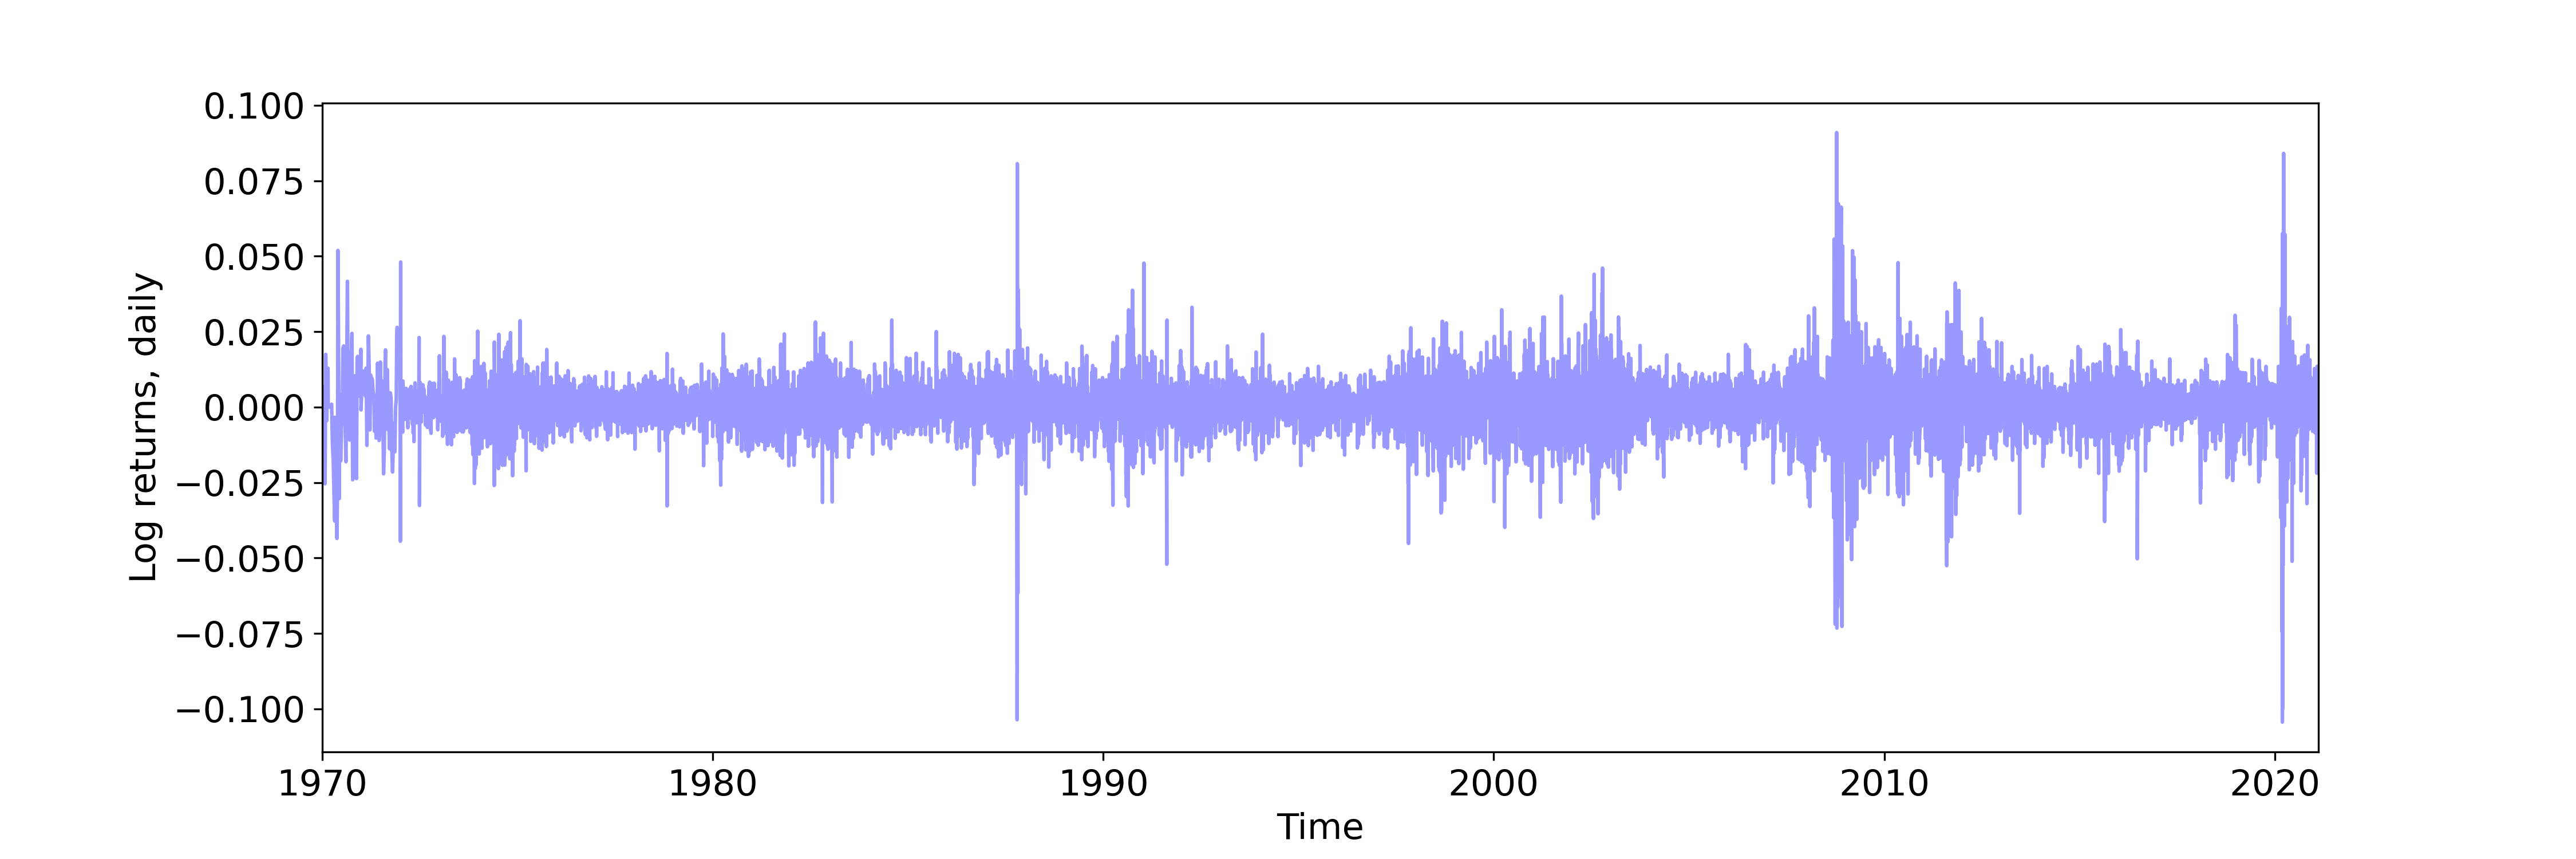
\includegraphics[width=0.65\textwidth]{analysis/data_description/images/MSCI_log_returns.png}
    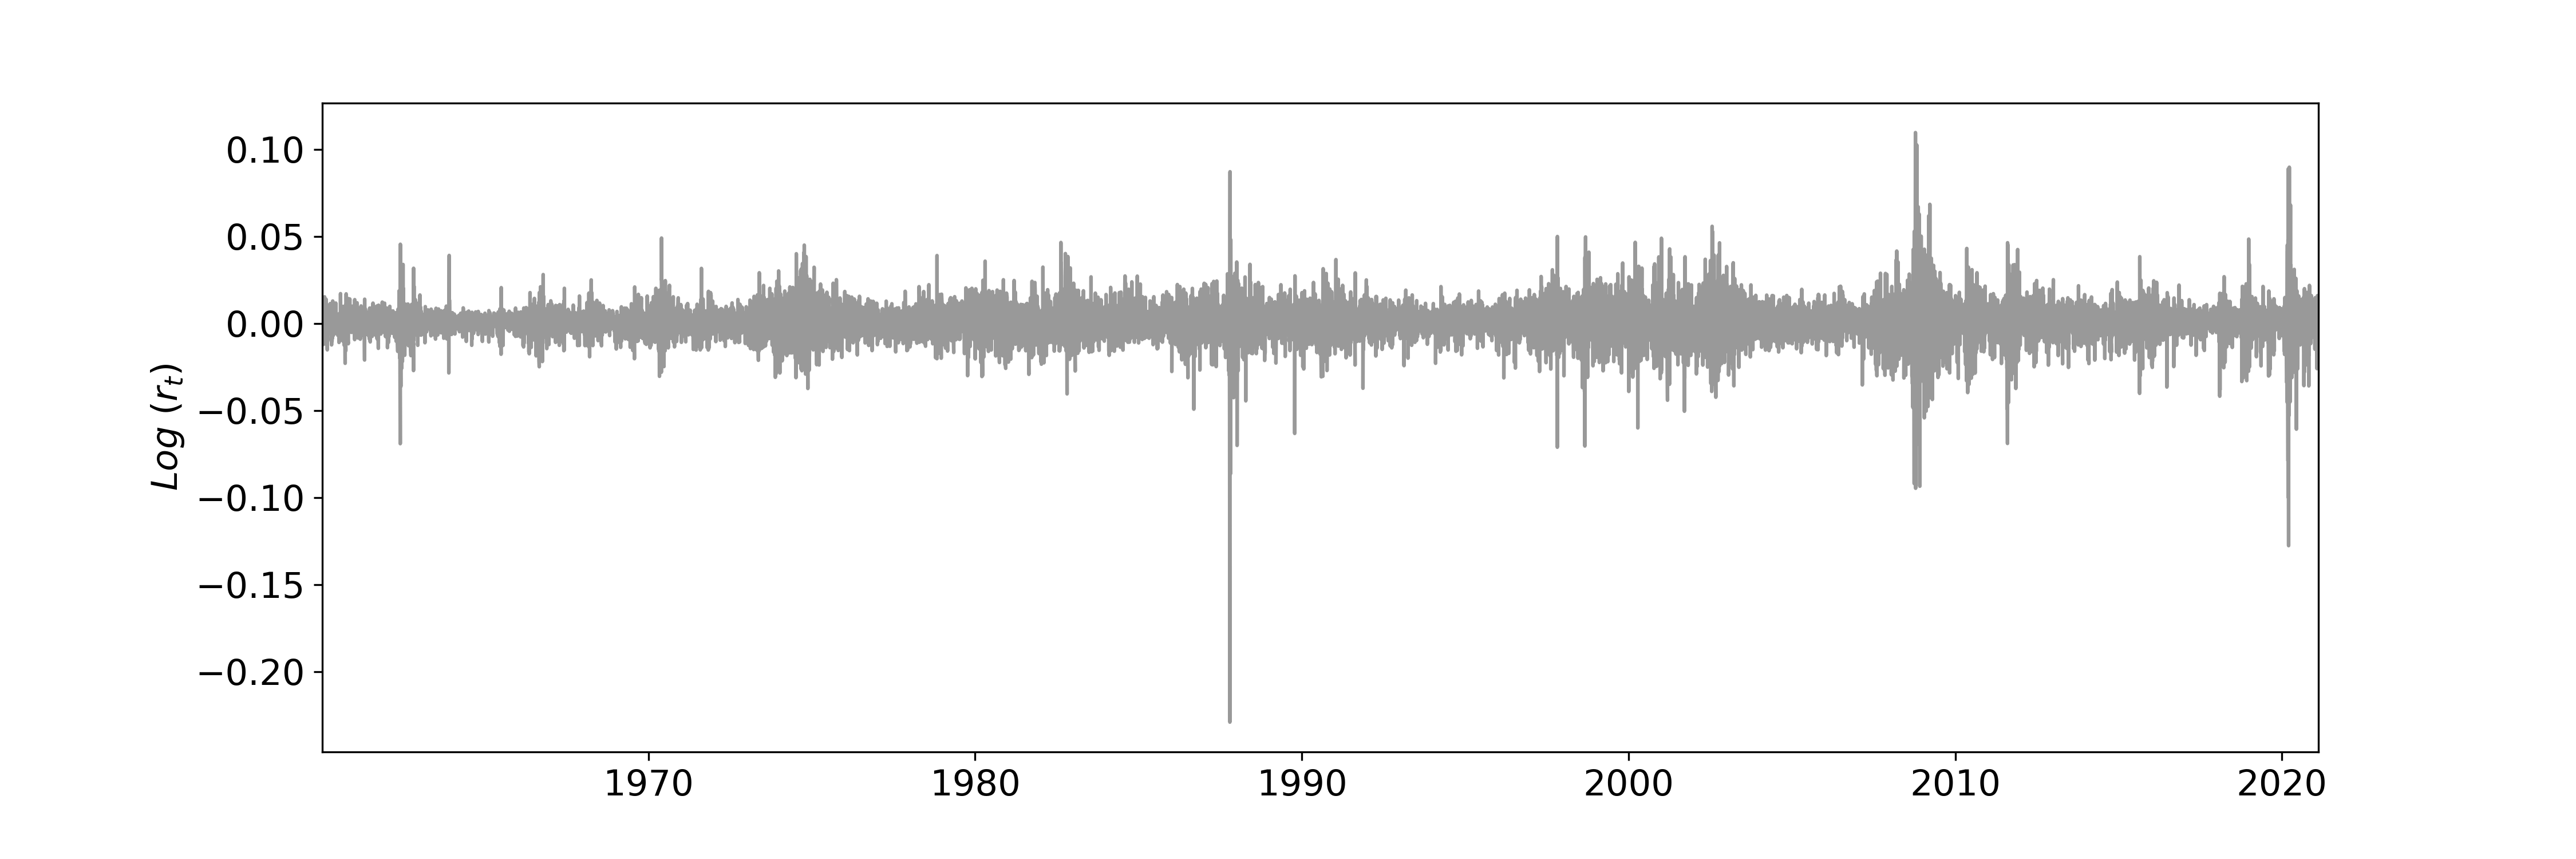
\includegraphics[width=0.65\textwidth]{analysis/data_description/images/SP500_log_returns.png}
    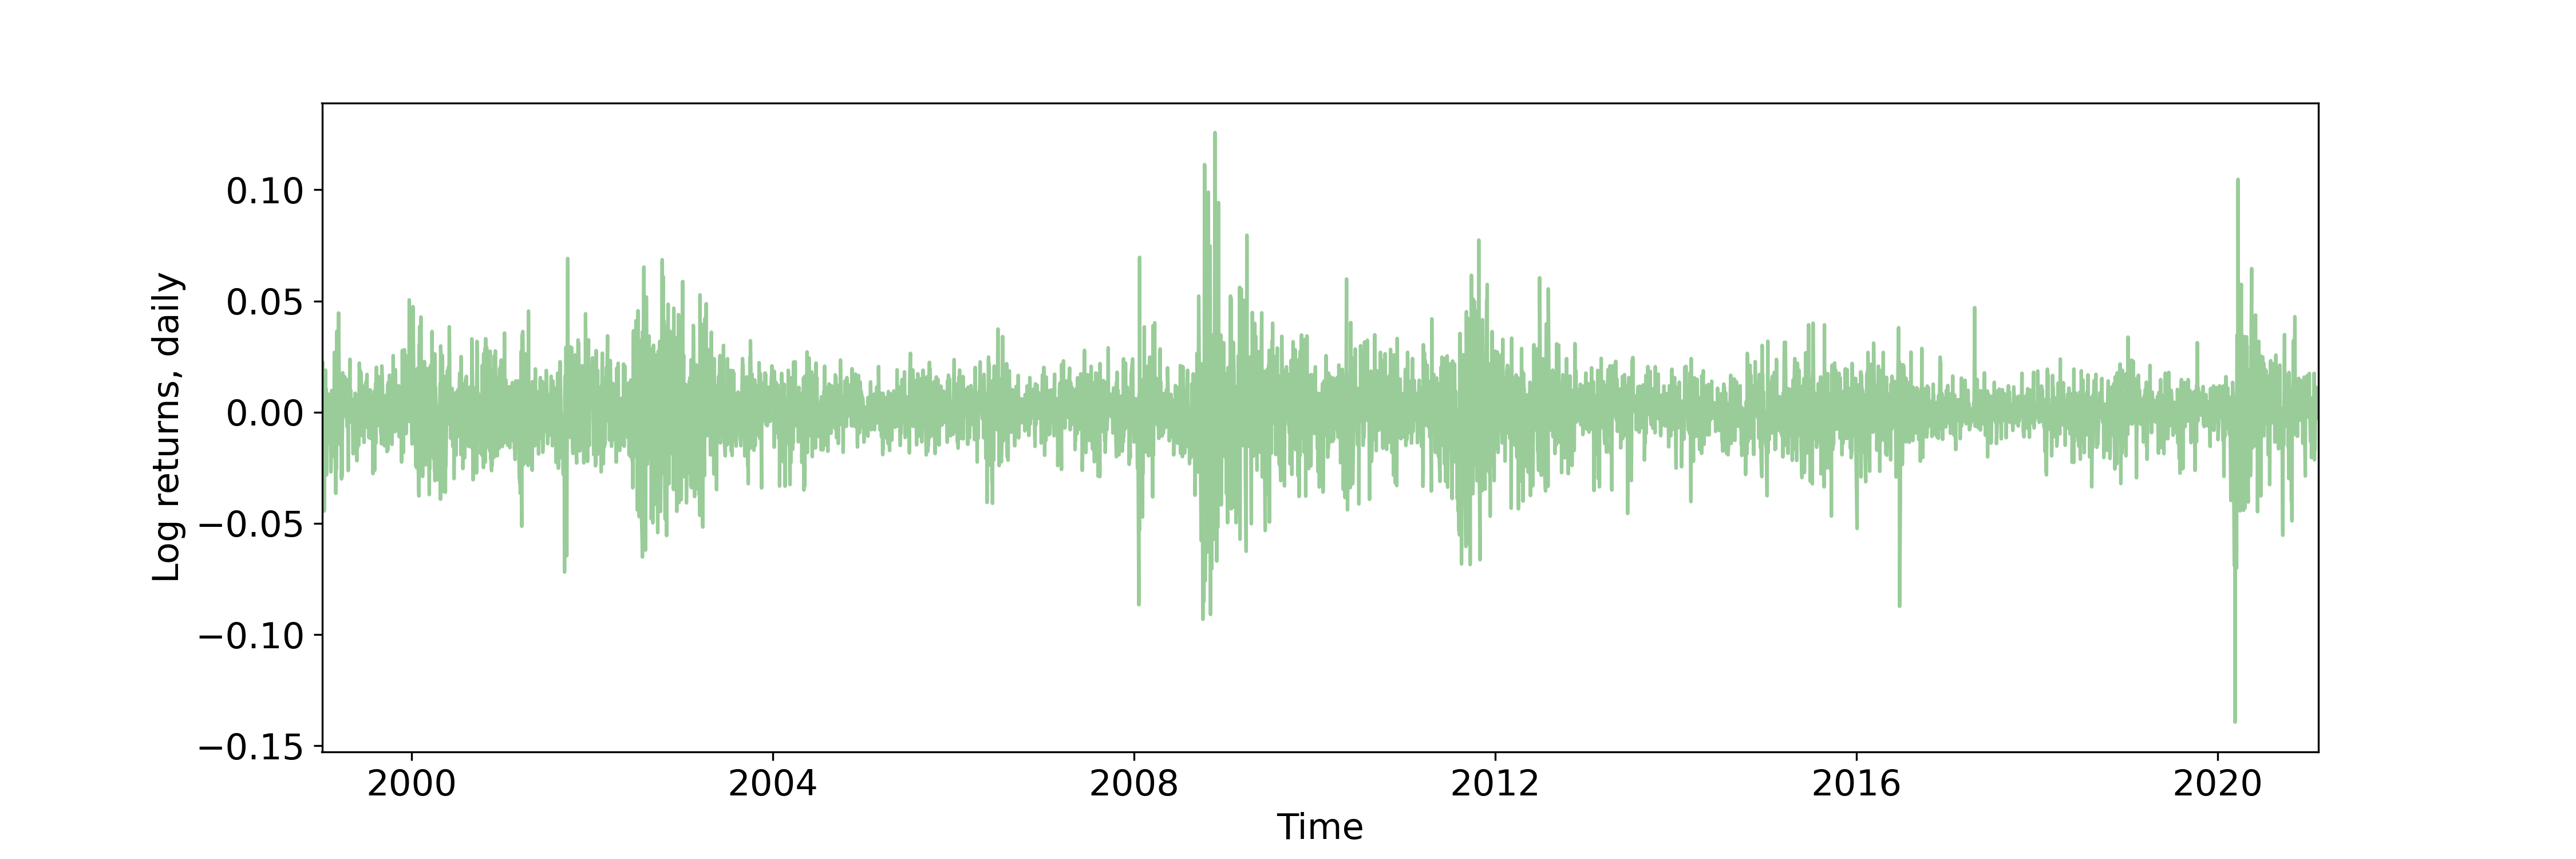
\includegraphics[width=0.65\textwidth]{analysis/data_description/images/DAX_log_returns.png}
    \caption{Log returns. MSCI, S\&P500 and DAX respectively.}
    \label{fig: log_returns_all_indices}
\end{figure}

%%% INDSÆT FIGUR AF LOG RETURNS FOR ALLE INDICES.

\label{subsection: distributional properties}

 
\subsection{Temporal properties}
\label{subsection: temporal properties}
It is evident by the plot of the log returns for the different indices in figure \ref{fig: log_returns_all_indices} that the log returns are characterised as mean stationary, since they fluctuate around a constant mean level close to zero for all three indices. Despite this, the log-returns series for all three indices are seen to be more volatile in some periods. The effect that large prices movements tend to be followed by other large price movements, but not necessarily in the same direction, is known as volatility clustering (Cont, 2001). 

Particularly the MSCI World and S\&P 500 index appear to have increasing volatility throughout time, whereas the DAX 30 appears to have similar or slightly contracting volatility levels. This is not surprising as the MSCI World and S\&P 500 index include observations beginning from the 1970s and 1960s respectively. During these times, there were no active derivative markets and much fewer actors had direct access to trading financial instruments. As such, markets were simpler, less risky and thus characterised by an overall lower level of volatility. 

\begin{figure}[H] 
    \centering
    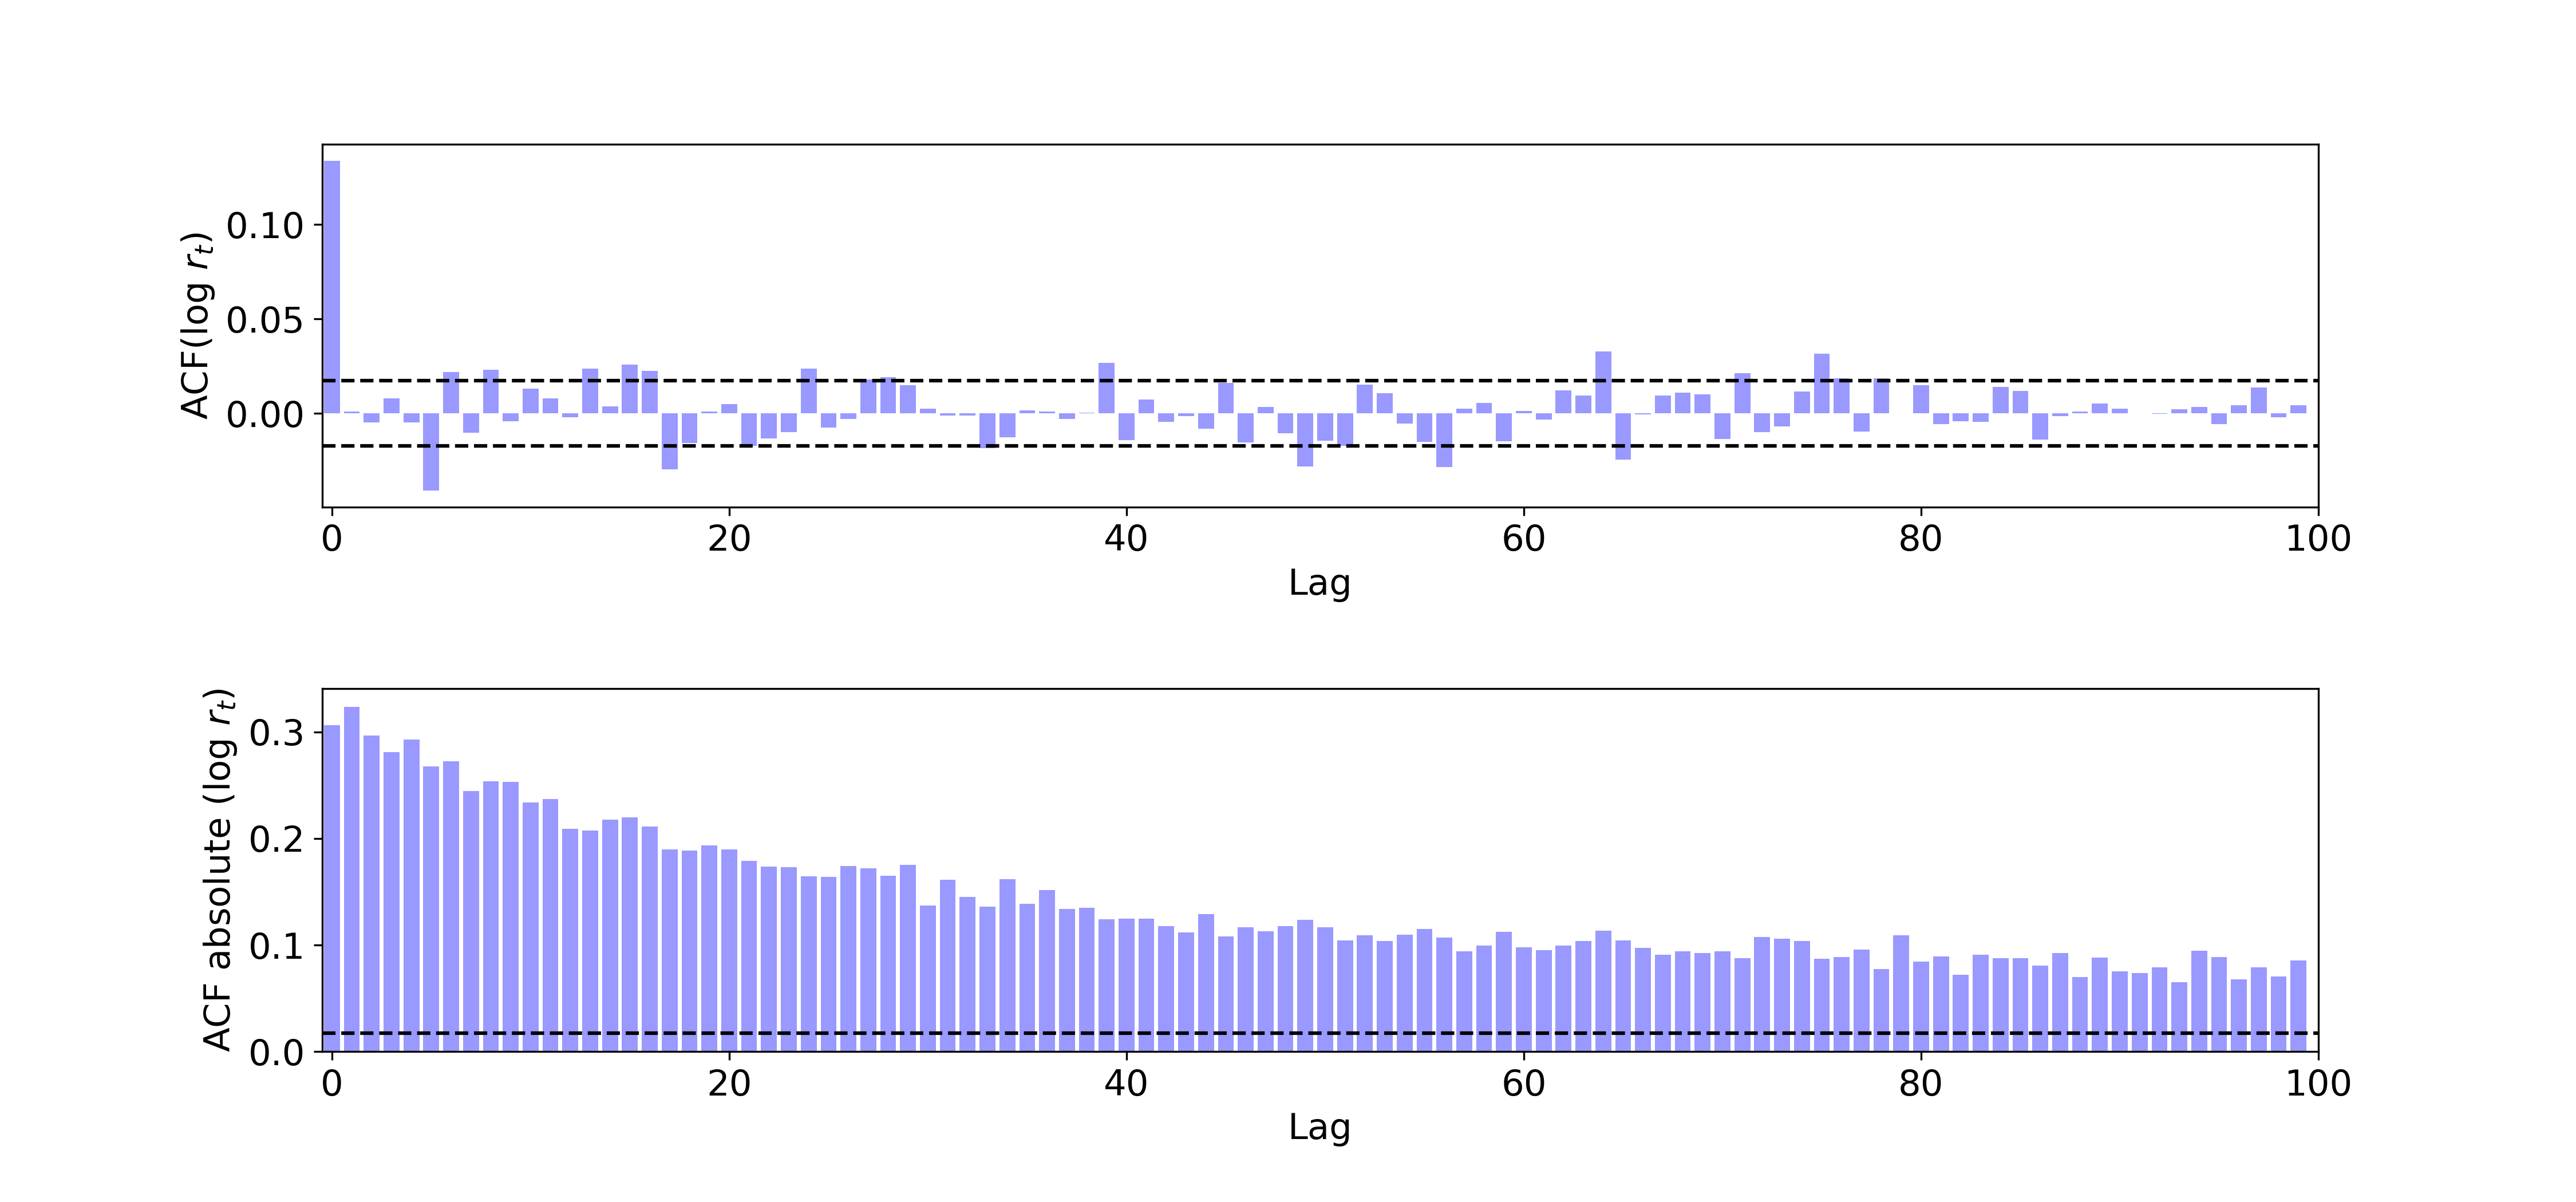
\includegraphics[width=0.65\textwidth]{analysis/data_description/images/MSCI_ACF.png}
    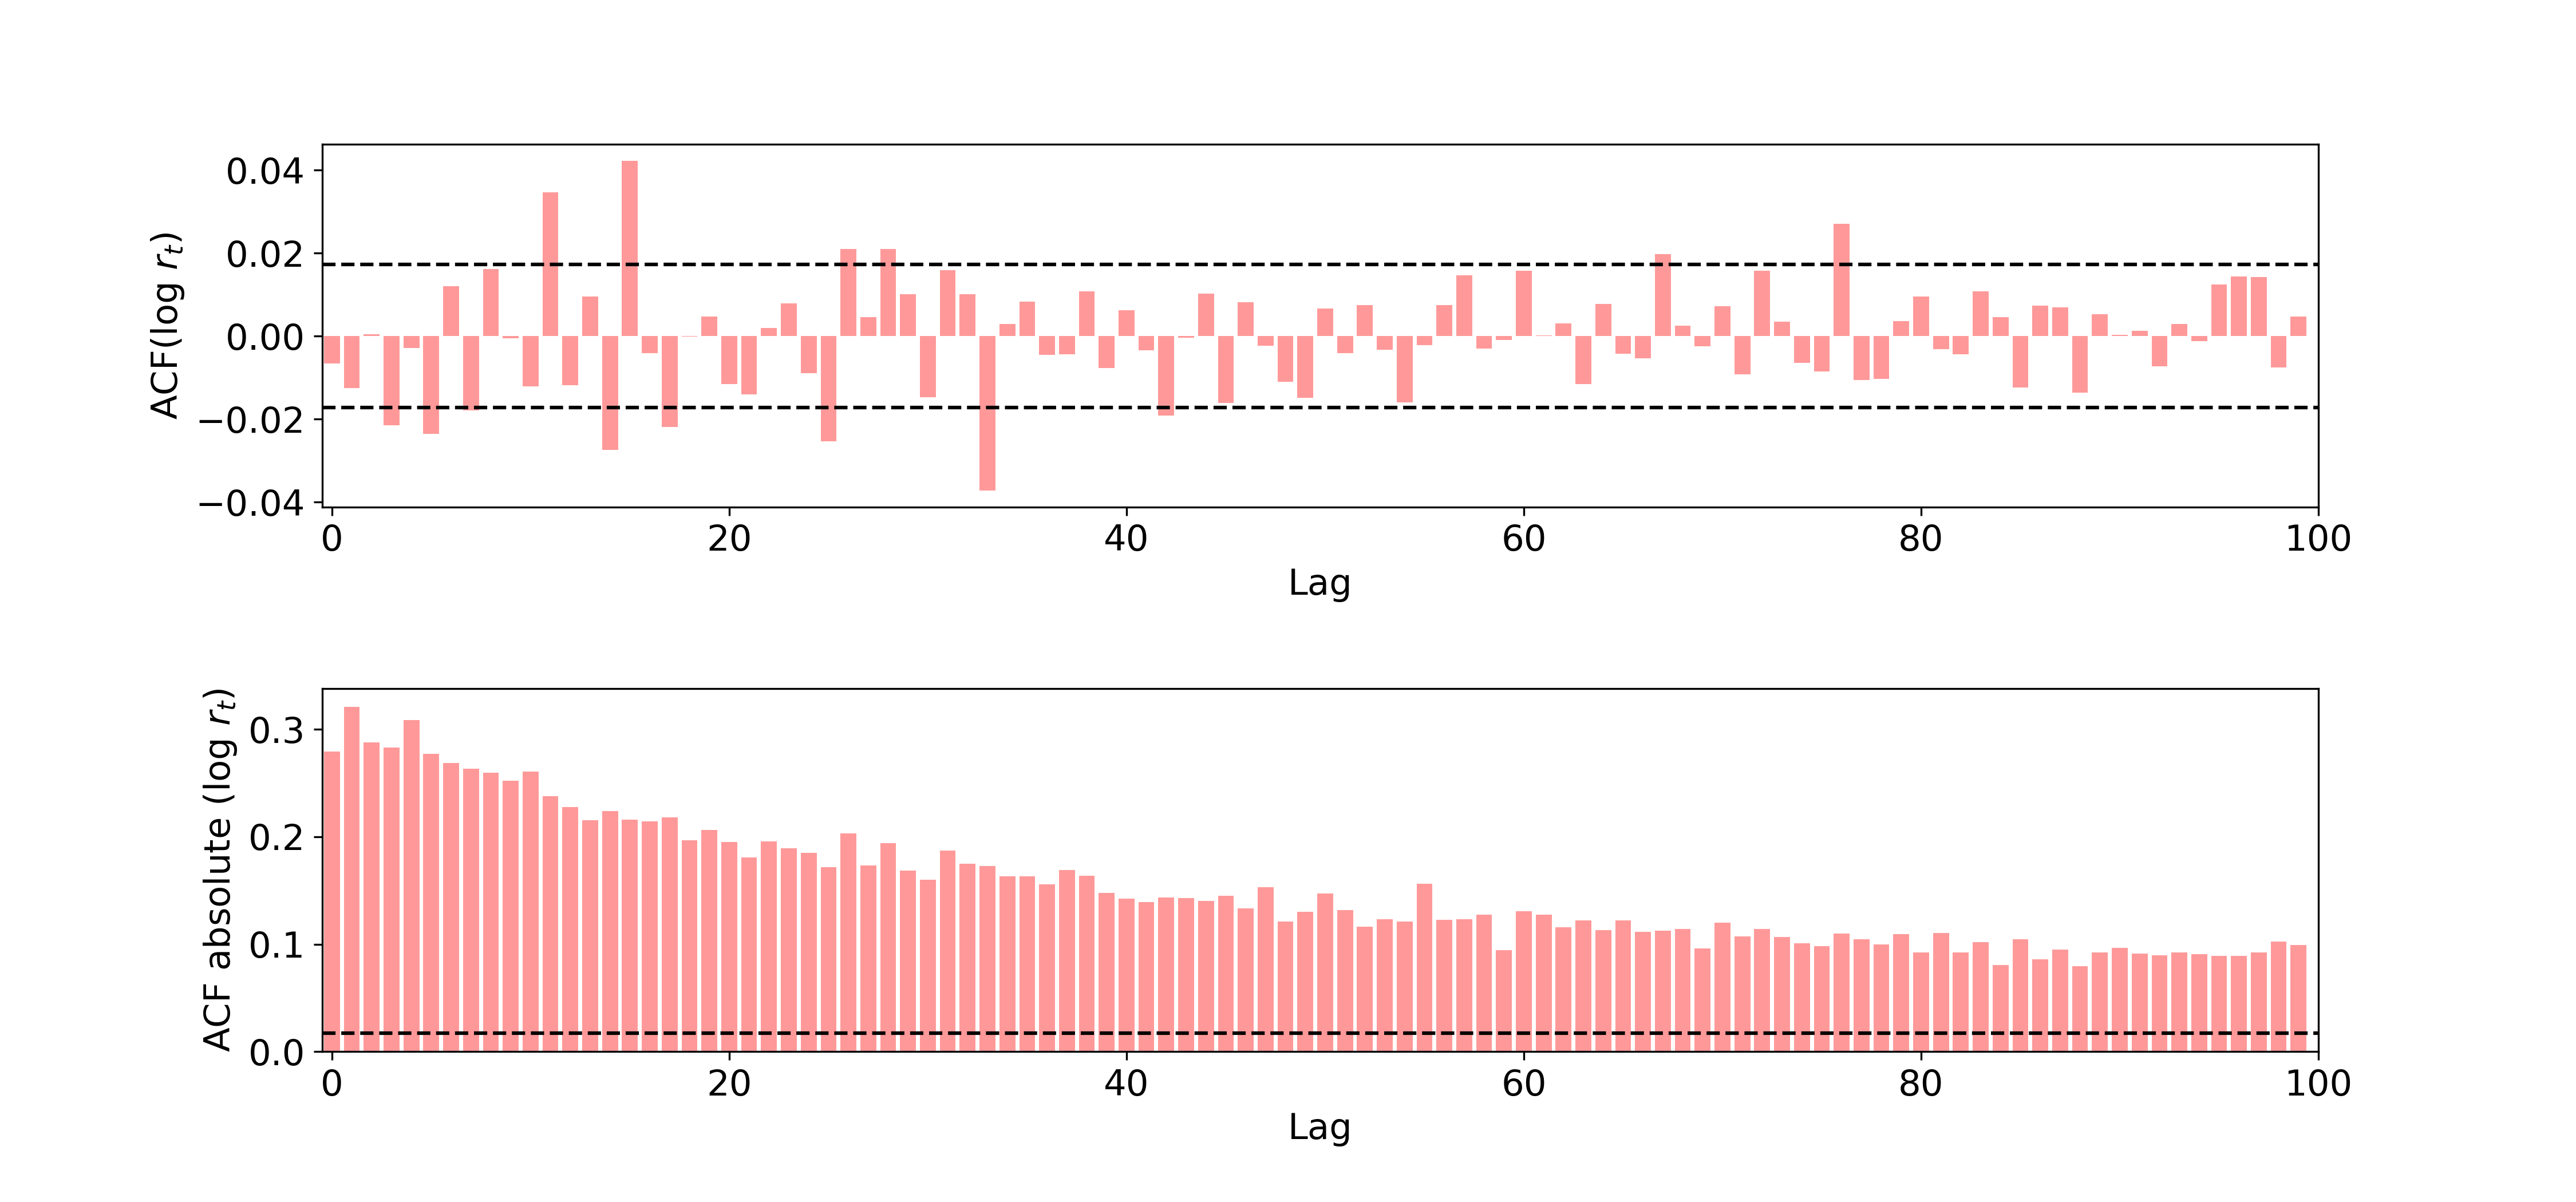
\includegraphics[width=0.65\textwidth]{analysis/data_description/images/SP500_ACF.png}
    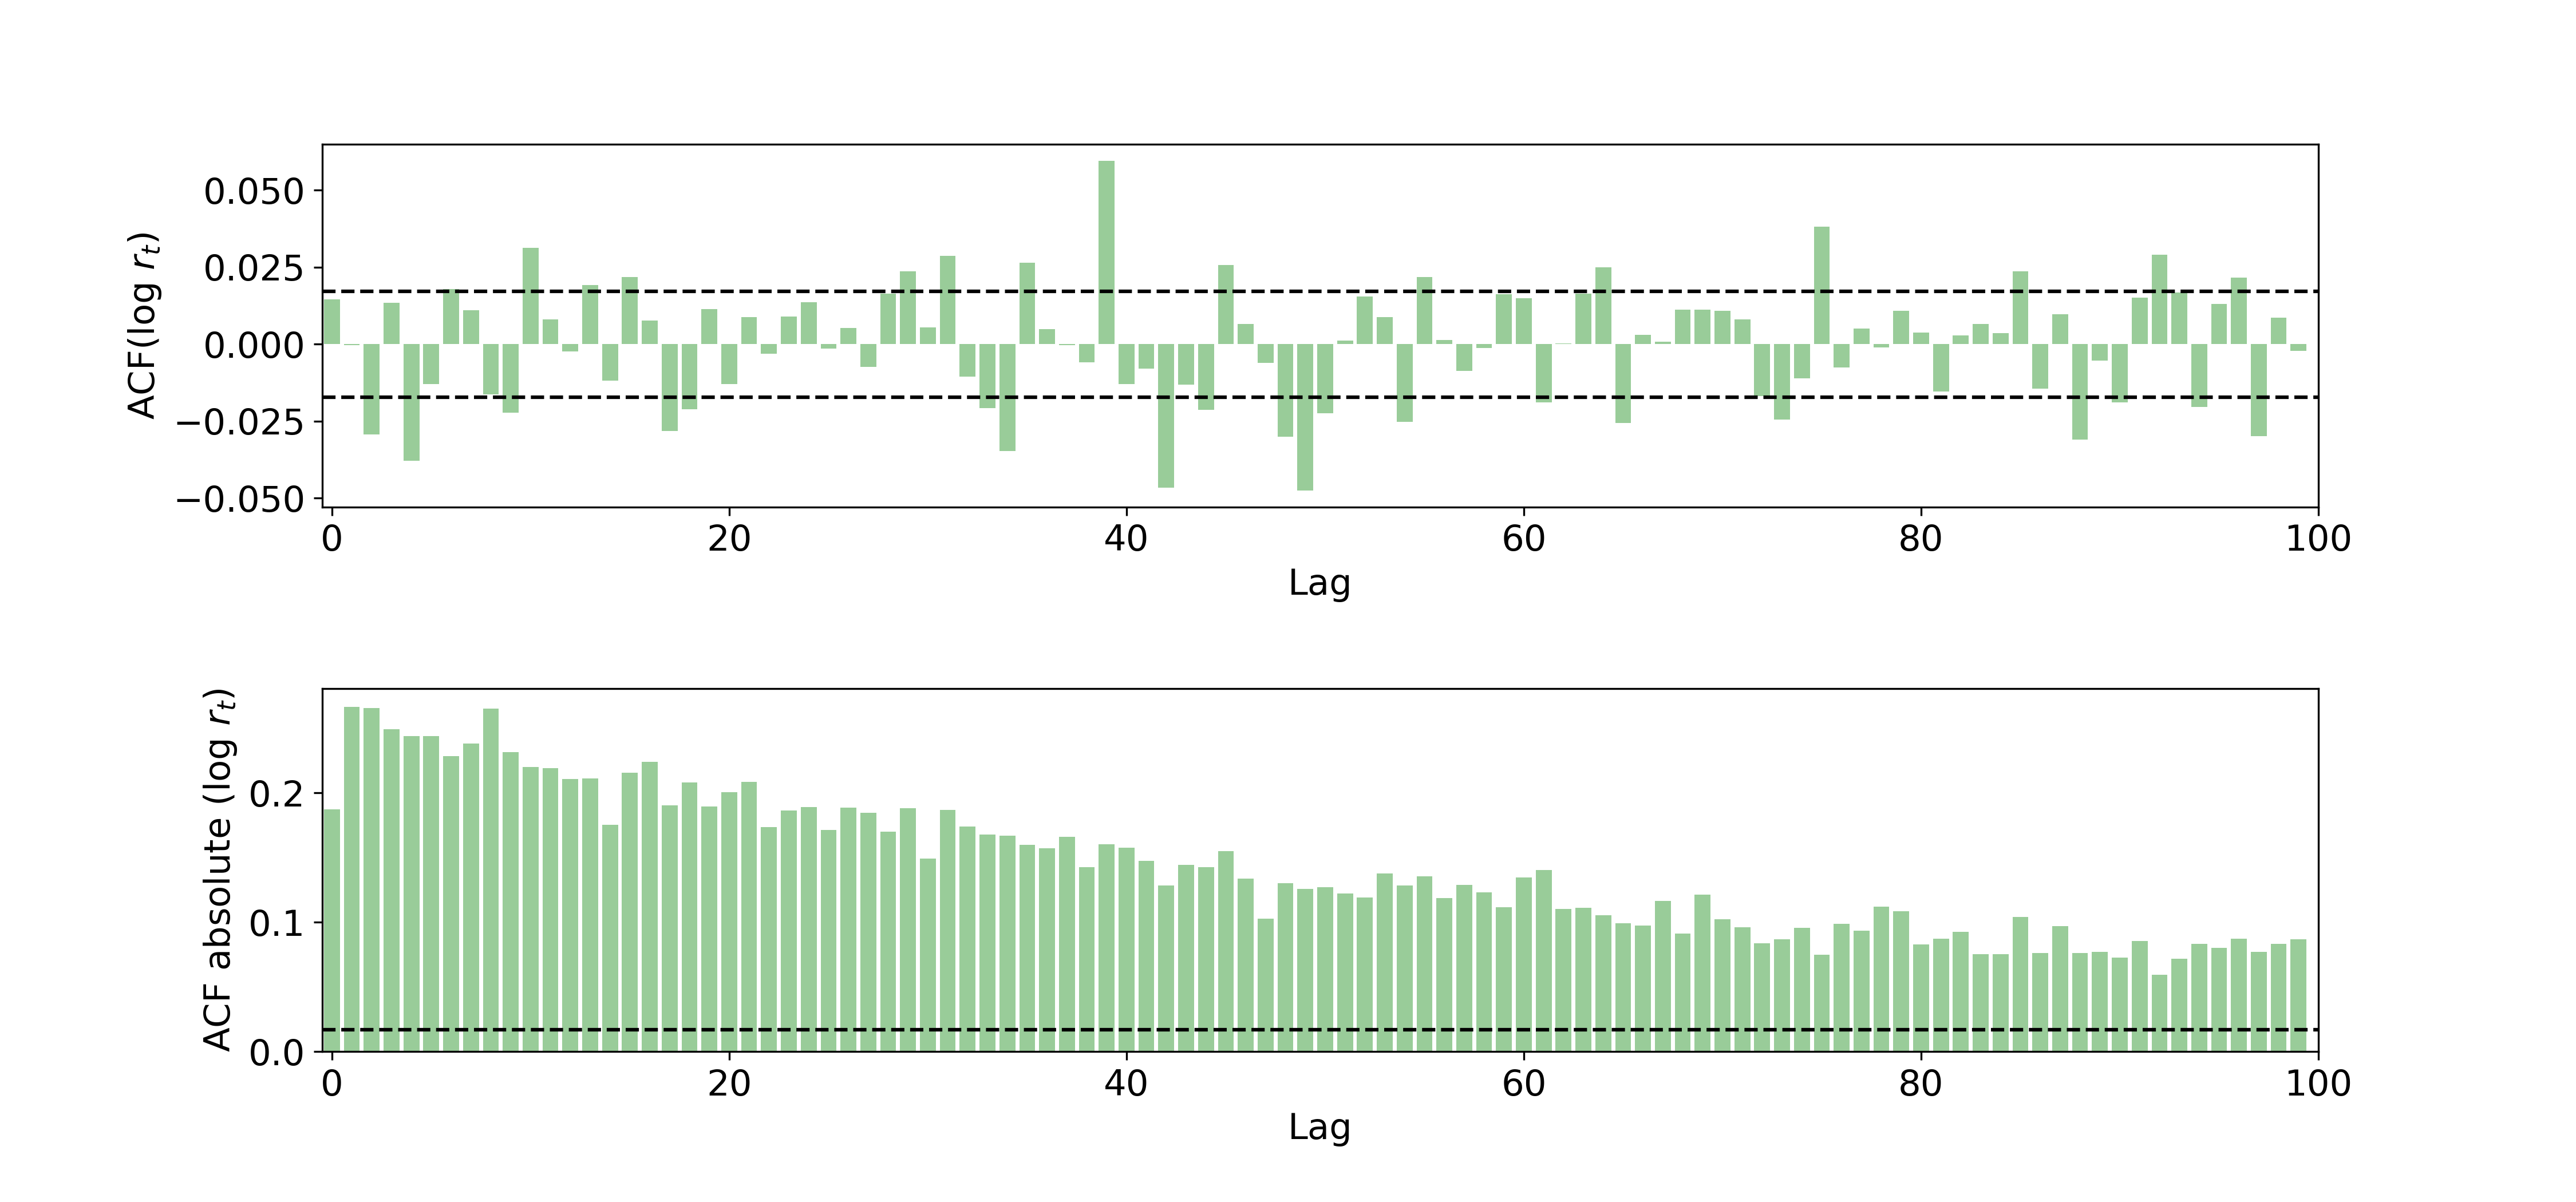
\includegraphics[width=0.65\textwidth]{analysis/data_description/images/DAX_ACF.png}
    \caption{ACF and absolute ACF. MSCI, S\&P500 and DAX respectively. The dashed black line is the 95\% significance level.}
    \label{fig: ACF_all_log_returns}
\end{figure}

The autocorrelation functions (ACFs) for the log-returns and the absolute log returns are shown in figure \ref{fig: ACF_all_log_returns}. The first-order autocorrelation is only significant for the MSCI World index. However, the reader should note that the ACF is time-varying, thus if one were to zoom in on a narrower time-period it is highly probable that the first-order autocorrelation could be significant for all indices. 

The absolute ACFs show significant autocorrelation that persists all the way up to lag 100 for all the selected indices. This suggests that financial returns exhibit a memory component, thereby making volatility somewhat predictable. As such, the long memory of the absolute log-returns is closely related to the previously described volatility clustering from figure \ref{fig: log_returns_all_indices}.

Conclusively, the reader should note that the correlation among the indices are stronger at the times of high market volatility. This is perhaps not surprising since the indices are made up of stocks, however, it highlights that diversification based on investing in different sectors or geographical areas may not materialize precisely when an investor needs it the most. The impact would most probably be less significant if one were to compare a stock index with a bond index, since the correlation would be lower, especially during periods of high volatility. Despite the fact that correlations increased in high volatility markets, there are definitely benefits related to diversification between asset classes.
    \newpage

\section{Reproducing stylized facts with HMMs}
\label{Section: Stylized facts}

\textbf{Still need to figure out whether to move data section to here, deleting data section completetly or keeping it...}

\textbf{Current decoding/prediction is not really used for anything. Consider deleting or changing the analysis. Basing the section on smoothing probabilities in the rolling model might be better than showing predictions since this is what is used in forecasting in MPC framework.}

The previous section involved tuning the \jump and \mle estimators followed by an analysis showcasing how the models perform in a number of simulated environments. This section will build on the recently acquired knowledge to train the models on financial data. As such, the purpose of this section is to analyze the estimator's fit to financial returns, which is mostly analyzed by evaluating the models' ability to reproduce some well established stylized facts. As highlighted throughout section \ref{section: Data} the normal distribution provides a poor fit for financial returns and it is very difficult to train models capable of yielding the same distributional and temporal properties as those of financial returns (Cont, 2001). Researchers, including Granger \& Ding (1995b), Cont (2001) and Malmsten \& Teräsvirta (2010), have found a variety of different stylized facts that are persistent across asset returns. 

Building on the stylized facts of Granger \& Ding (1995b), Rydén et al. (1998) showed how a mixture of Gaussian distributions, theoretically can satisfy the stylized facts and subsequently attempted to fit a Gaussian HMM to S\&P 500 log returns. Rydén et al. (1998) found that most of the stylized facts could in fact be well reproduced by a Gaussian HMM, yet many of the stylized facts had to be somewhat relaxed. In particular, the researchers found the slow decay of the absolute returns to be the hardest to reproduce. This is due to the fact that HMMs by design exhibit exponential decay in their absolute autocorrelation functions. Furthermore, by splitting their data into 10 sub-samples of 1700 observations, Rydén et al. (1998) found significant changes to underlying data-generating process. Furthermore, Bulla et al. (2011) considered a similar analysis, however, they also included HMMs fitted on conditional t-distributions for which they achieved a better fit in regards to some of the stylized facts, especially those regarding higher order moments. Yet, they still found significant changes from one sub-sample period to the next, not only in their models but in the empirical data as well. As such, it can be concluded that the results from both these studies imply that the data merely fluctuates around the stylized facts of introduced by Granger \& Ding (1995b).

One inherent issue with both these authors' approach is that when dividing the empirical data into sub-samples of 1700 periods, it becomes more challenging to estimate long-memory effects from the models. Furthermore, it is also a very rough discretization of the data, which makes it more difficult to assess how the model parameters evolve across time. More recent research has tried to alleviate this with either online or rolling models such as Nystrup (2017), though he only considered the HMMs ability to reproduce squared autocorrelation functions and thus omitted analysing any of the other properties established by Granger \& Ding (1995b).

As a result, the contribution of this section to the current literature will be the estimation of rolling HMMs, through the \mle and \jump approach, as well as such models' ability to reproduce the stylized facts of Granger \& Ding (1995b). The preliminary findings indicate that the rolling models generally have a much slower decay in its absolute autocorrelation function compared to the static models of Rydén et al. (1998) and that the distributional properties are well reproduced across the data period\footnote{
With some exceptions to kurtosis in periods around Black Monday, the Financial Crisis and the COVID-19 outbreak.
}
Additionally, this is also the first study to consider how well HMMs estimated through the \jump approach reproduce the stylized facts.

The rest of the section is organized as follows. Firstly, the thesis investigate the data of which the rolling models are trained after which an overview of the rolling estimation and the model parameters is provided. Secondly, the stylized facts established by Granger and Ding (1995b) are briefly reviewed, after which these stylized facts are sought reproduced with the \mle and \jump models. When testing the models' ability to reproduce the stylized facts the distributional properties are initially estimated followed by the temporal properties. \textbf{Finally, both model's state predictions are shown together with their smoothing probabilities.}


\subsection{Data - The S\&P 500}

\textbf{Der skla noteeres at observationer som Black Monday er droppet sammen med 3 andre ekstreme observationer - se sektion 6.}

\textbf{Afsnittet bør rykkes ned til sektion 6 og forkortes. Jeg syntes figurerne over dist. og temp. properties skal i appendiks da det alligevel bliver nøgternt gennemgået i sektion 6. Alternativt skal de være en del af introen som argument for hvorfor returns er svære at modellere. Vi kan stadig beholde lidt af teksten og så henvise til figuren i appendiks.}

\textbf{Priser og returns skal merges sammen i en figur over og under hinanden. - tænker også at y-aksen på priser kan uddgøre 2/3 af højden på den figur, mens y-aksen på returns kan udgøre 1/3 af højden.}

The S\&P 500 is a stock index comprising 500 companies from the U.S. which was founded in 1957, however, the index dates back all the way to 1923 where it tracked approximately 90 stocks. The stocks that make up the index are selected by a committee which includes representation from all major segments in American industry. As such, contrary to prevailing public sentiment, the index is not simply made up of the 500 largest companies in the U.S. The S\&P 500 is a market-capitalization weighted index in which the 10 largest companies account for 27.5\% of the capitalization as per December 2020. Figure \ref{fig: SP500_index} showcases the development of the S\&P 500 index since origination as well as the log returns. 
 
\begin{figure}[H] 
    \centering
    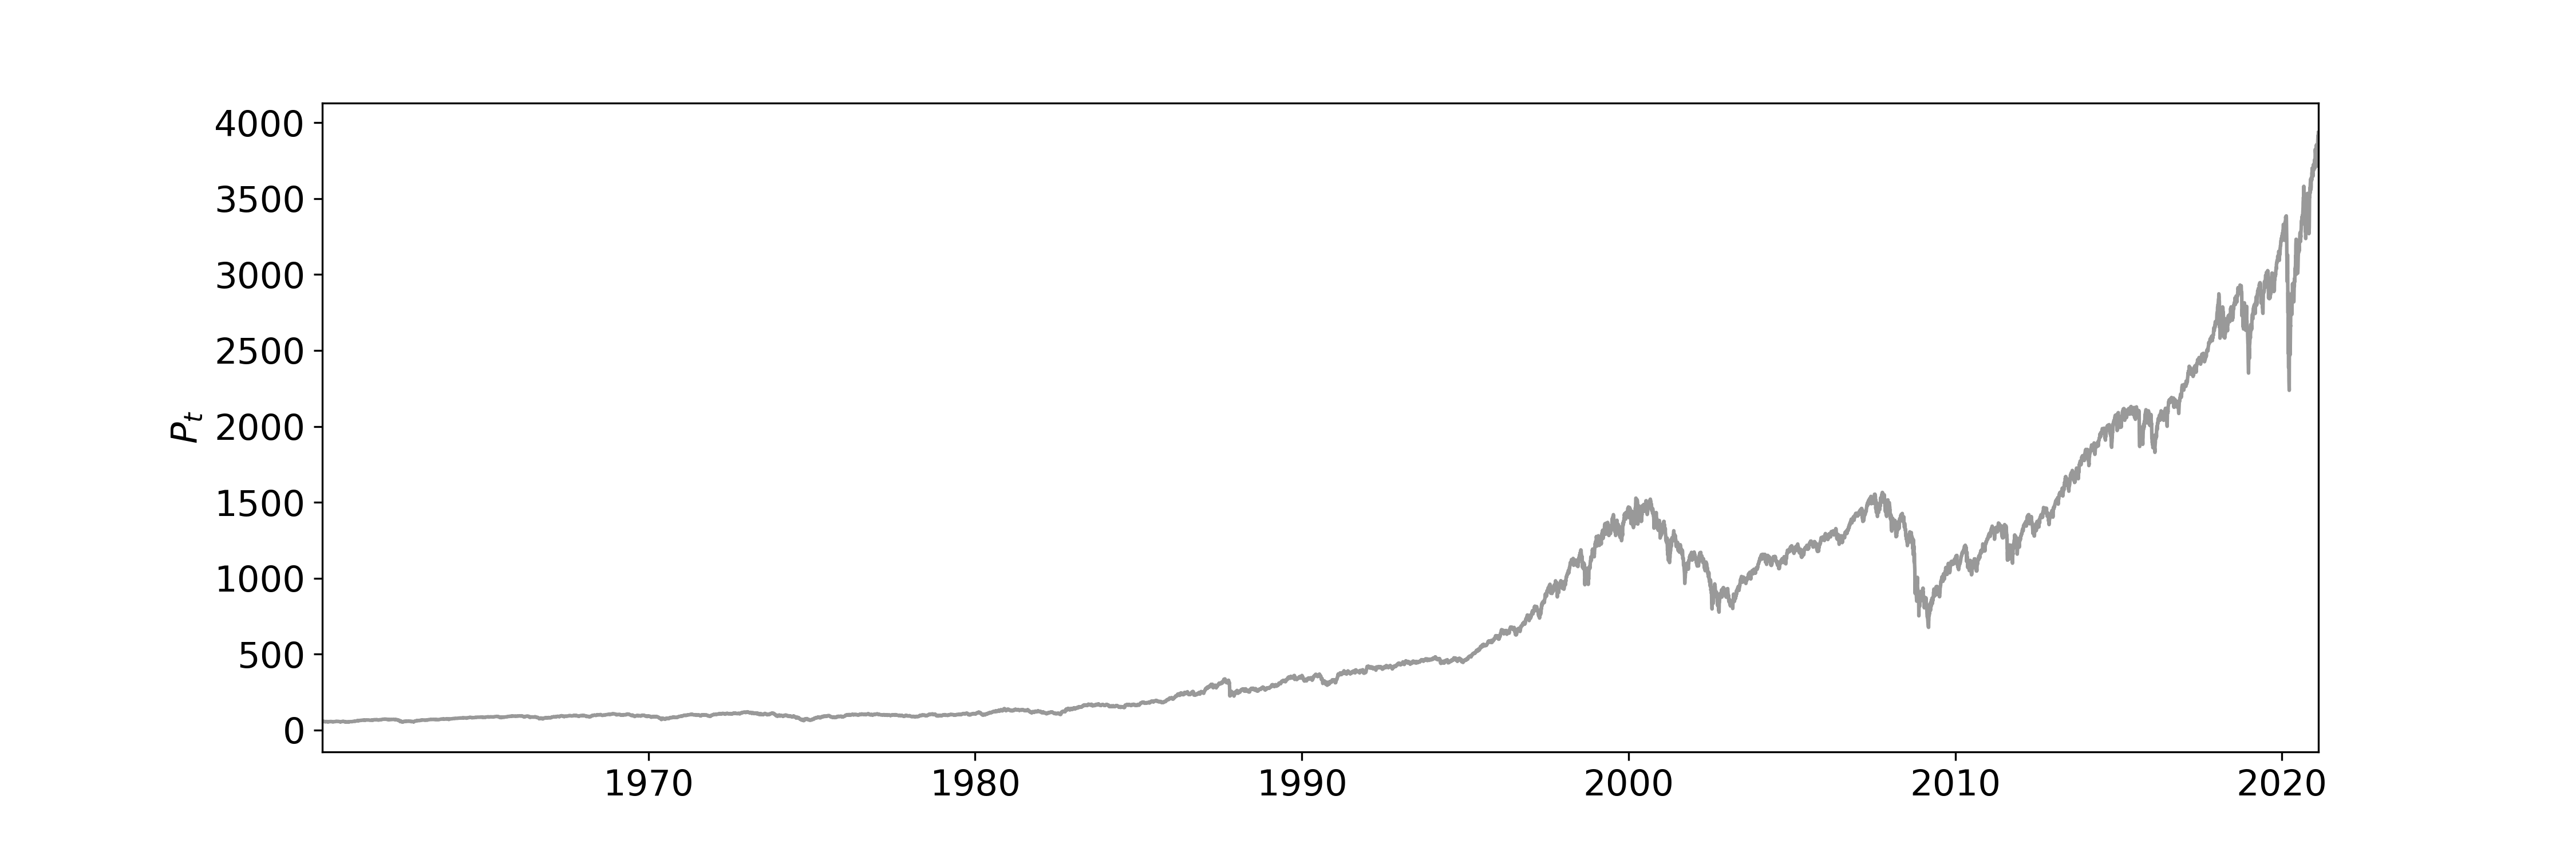
\includegraphics[width=1\textwidth]{analysis/data_description/images/SP500_index.png}
    \caption [Development of the S\&P 500] {Development of the S\&P 500 for the period 01/04/1960 to 12/02/2021.}
    \label{fig: SP500_index}
\end{figure}

The log returns are derived as $r_t = log(P_t) - log(P_{t-1})$, where $P_t$ is the adjusted closing price of the index on day $t$ and $\log$ is the natural logarithm. This is done since log returns provides a better overview of the historical market events that have caused extreme observations, for instance the Black Monday event of October 1987 which saw the S\&P 500 index drop by 22.9\% in a single day. This event is not particularly visible from the price series plot. Furthermore, it is rather impractical to try and use prices to estimate models, since stock and index prices are impossible to predict, hence a model estimation procedure should not be trained on price data.

It is evident from figure \ref{fig: SP500_index} that the 44 years of data has been impacted by the major market movements including Black Monday in October 1987 as well as the dot-com bubble of the late 90s and early 2000s. Furthermore, the attractive bull market leading up to the GFC has been well-captured by the development of the S\&P 500 Index. Lastly, the long bull market following the GFC as well as the recent COVID-19 recession appears to be well-captured by the S\&P 500 Index, thereby indicating that it is adequate for model estimation purposes. In addition, the development following the electronification of financial markets is evident since many actors, including private investors, gained access to the financial markets due to the advancement of technology in the late 90s and early 00s. This is also clearly visible from figure \ref{fig: SP500_index}


From an overall return perspective it is evident that the S\&P 500 index has been subject to a variety of turbulent market periods including the dot-com bubble and most recently the GFC and COVID-19 recession. Interestingly, the S\&P 500 index only recovered from the dot-com bubble a few months prior to the financial crisis of 2008. In the period following the financial crisis the S\&P 500 has been performing increasingly well resulting in an upward trajectory until the recent COVID-19 correction, after which the index reached the present all time high. The fact that the S\&P 500 index has captured the most recent and dramatic market turmoil throughout the last 60 years, further establish that it captures the varying nature of economic regimes. Furthermore, another neat property of the S\&P 500 is the fact that it dates back to 1957, hence there is a large amount of data that can be used to train the subsequent HMMs. For comparison, popular European indices like the DAX 30 originated in 1999, thus shortening the available data considerably.

Additionally, another the choice of relying on the S\&P 500 index for estimation purposes is based on the fact that it is a one of the leading American indices by market capitalization. Secondly, contrary to for instance the Nasdaq Composite Index, the S\&P 500 is not exclusively focusing on a specific sector like information technology, hence it should capture the economics trends across sectors accordingly. As such, the thesis treats it as a baseline index in terms of uncovering economic-regimes. The main critique of using the S\&P 500 index is that it exclusively entails American companies, however, from a macroeconomic perspective the U.S. economy serves as a fundamental leading indicator of how the remaining world economy is progressing, hence it is valid to argue that US stocks will be the first to be impacted by changing economic regime. Taking into consideration the aspect of early regime detection, this means that the fact that the index is composed purely of American companies serves as a strength. Furthermore, North American companies makes up almost 2/3 of alternative indices like the MSCI World, hence no matter which large popular index that will be used, there is bound to be a heavy skew and over-representation towards American stocks.


\begin{figure}[H] 
    \centering
    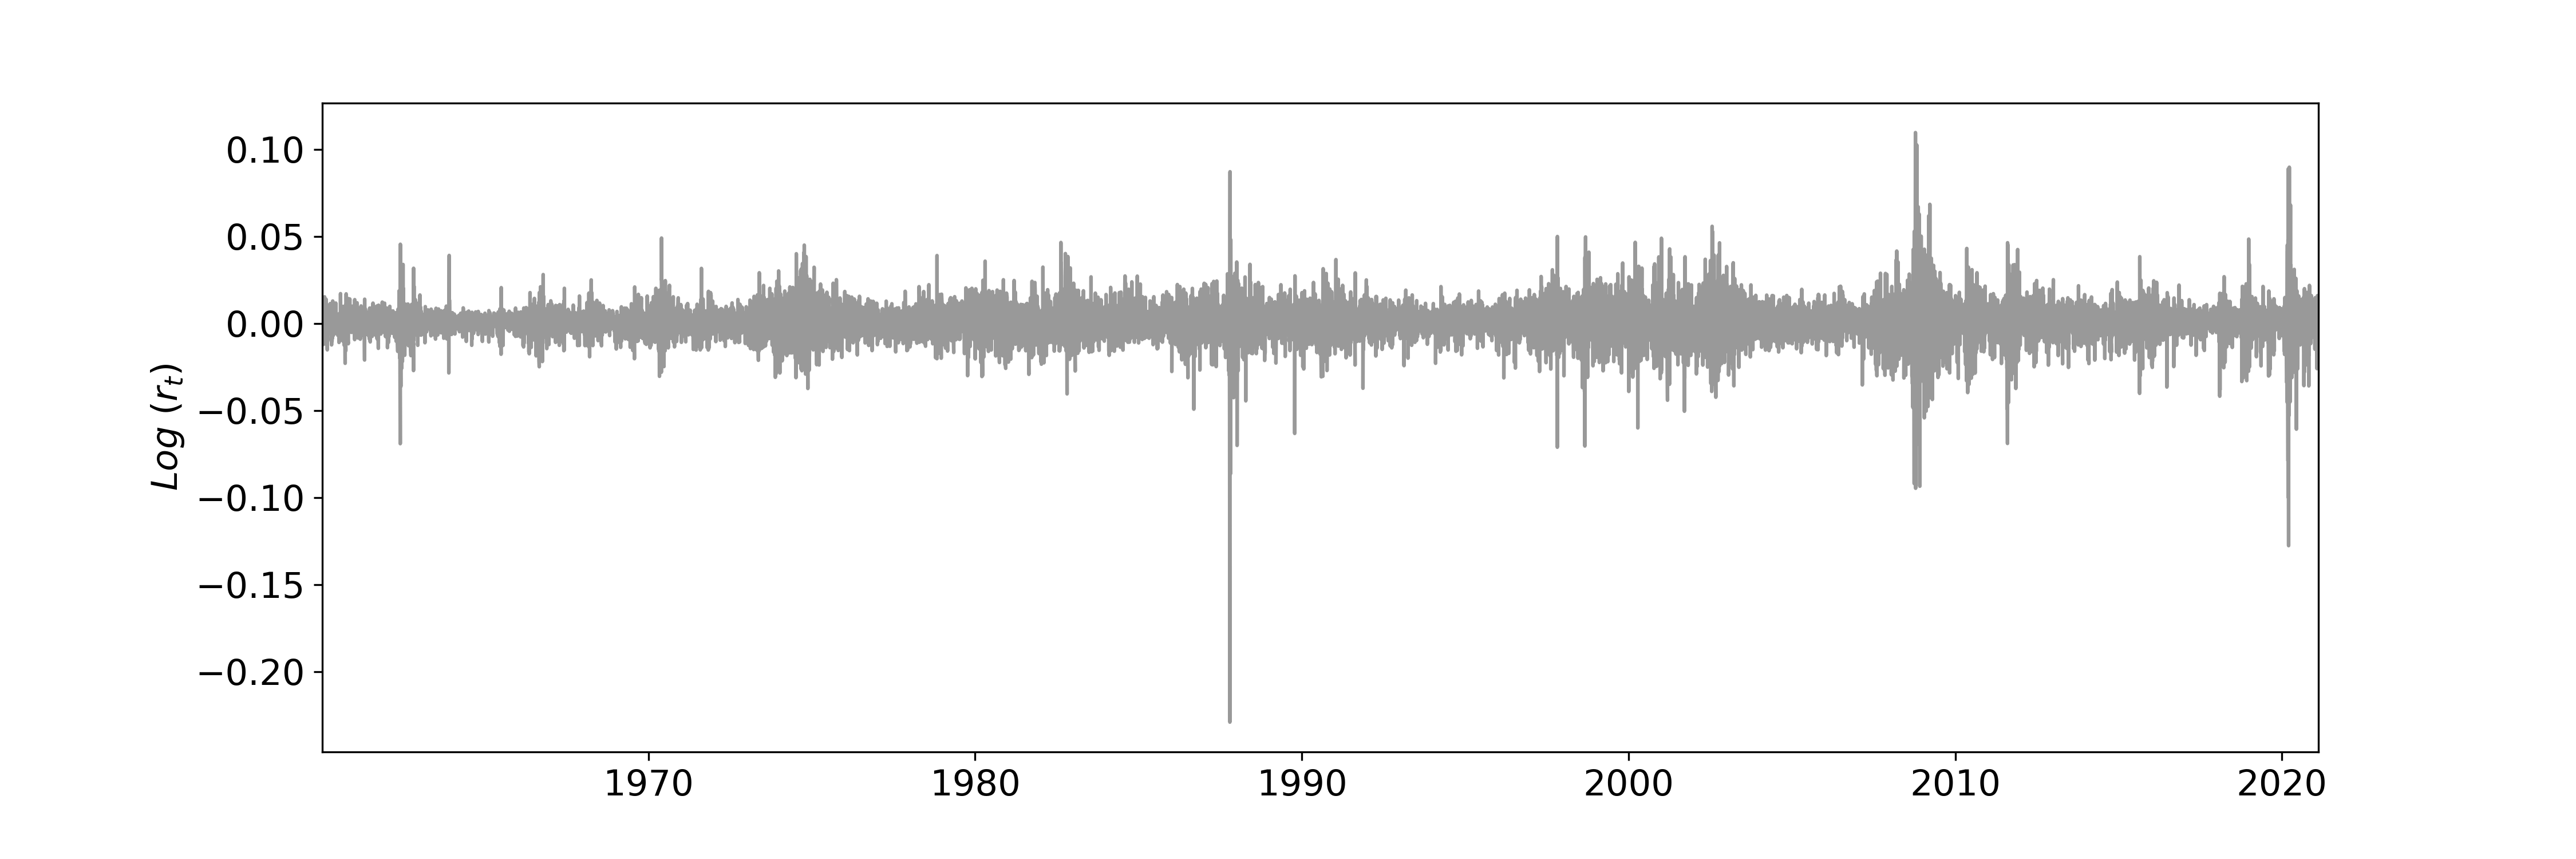
\includegraphics[width=1\textwidth]{analysis/data_description/images/SP500_log_returns.png}
    \caption [Plot of the log returns for the S\&P500 index across time] {Plot of the log returns for the S\&P500 index across time. \textbf{Figur skal være en del af priser. Ret y-akse}}
    \label{fig: log_returns_all_indices}
\end{figure}

In order to capture the summary statistics of the daily S\&P 500 log returns, as well as the annual Sharpe ratio and JB statistic, table \ref{tab:summary_stats_S&P500} has been constructed below. As such, it is apparent that the distribution is left skewed and strongly leptokurtic, however, this is not a surprising finding given the studies conducted by Granger \& Ding (1995b) as well as Cont (2001), in which identical stylized facts of financial returns were uncovered and explored substantially. The critical value for the Jarque–Bera test statistic at a 99.9\% significance level is 14.13, hence table \ref{tab:summary_stats_S&P500} clearly highlights that the Jarque–Bera test strongly rejects the hypothesis that the log returns of the S\&P 500 follow a Gaussian distribution.

\begin{table}[H]
\small
\caption{Summary statistics for the annualized S\&P 500 log returns.}
\centering
\begin{tabular}{c c c c c c c c c c} 
\hline\hline
Observations & Mean & STD & Skewness & Excess Kurtosis & Min & Max & Annual Sharpe & JB-stat \\
\hline
15,385 & 0.0709 & 0.1631 & -1.0353 & 23.8338 & -0.2290 & 0.1096 & 0.4350 & 27,926 \\
\hline
\end{tabular}
\label{tab:summary_stats_S&P500}
\end{table}
 

\subsection{Rolling estimation}
\label{Sec: rolling estimation}

The analysis now turns to estimating the \mle and \jump models on the S\&P 500 log returns covering the period 1960-2020. It should be noted that four very extreme observations\footnote{The observations include Black Monday, two trading days during the financial crisis and one observation during the outbreak of Covid-19.}
have been replaced with $\pm$ 6 times the standard deviation of the data. An important result from the simulation study was that the models became more stable with larger sample sizes in which the parameters generally appeared to stabilize between samples of 1000 and 2000 observations. As already mentioned, the window length is essentially a hyper-parameter that can be tuned and the exact choice boils down to a trade-off relationship between bias and variance. A shorter rolling window will, all else equal, result in a faster adaption to changes in the underlying economic regimes but the estimate will be more noisy as fewer observations are used when deriving the model parameters. This might result in the model adapting to "wrong" signals, which might affect the underlying trading strategy by decreasing risk-adjusted returns. A rolling window of 1700 days will be considered in this analysis as the model parameters should generally be stable at this length and this also makes it appropriate to draw direct comparisons to previous studies including Rydén et al. (1998), Bulla et. al (2011) and Nystrup (2017).

The estimation procedure for the rolling model is as follows. For each time step $t$ an HMM is estimated by the \mle and \jump procedures using the previous 1700 daily log returns. Once trained, the rolling window moves one time period forward to $t+1$ and repeats the procedure. The results of the rolling estimation for the \mle and \jump models based on a 2-state Gaussian HMM are shown in figure \ref{fig: MLE estimation rolling parameters} and \ref{fig: Jump estimation rolling parameters} respectively.

\begin{figure}[H] 
    \centering
    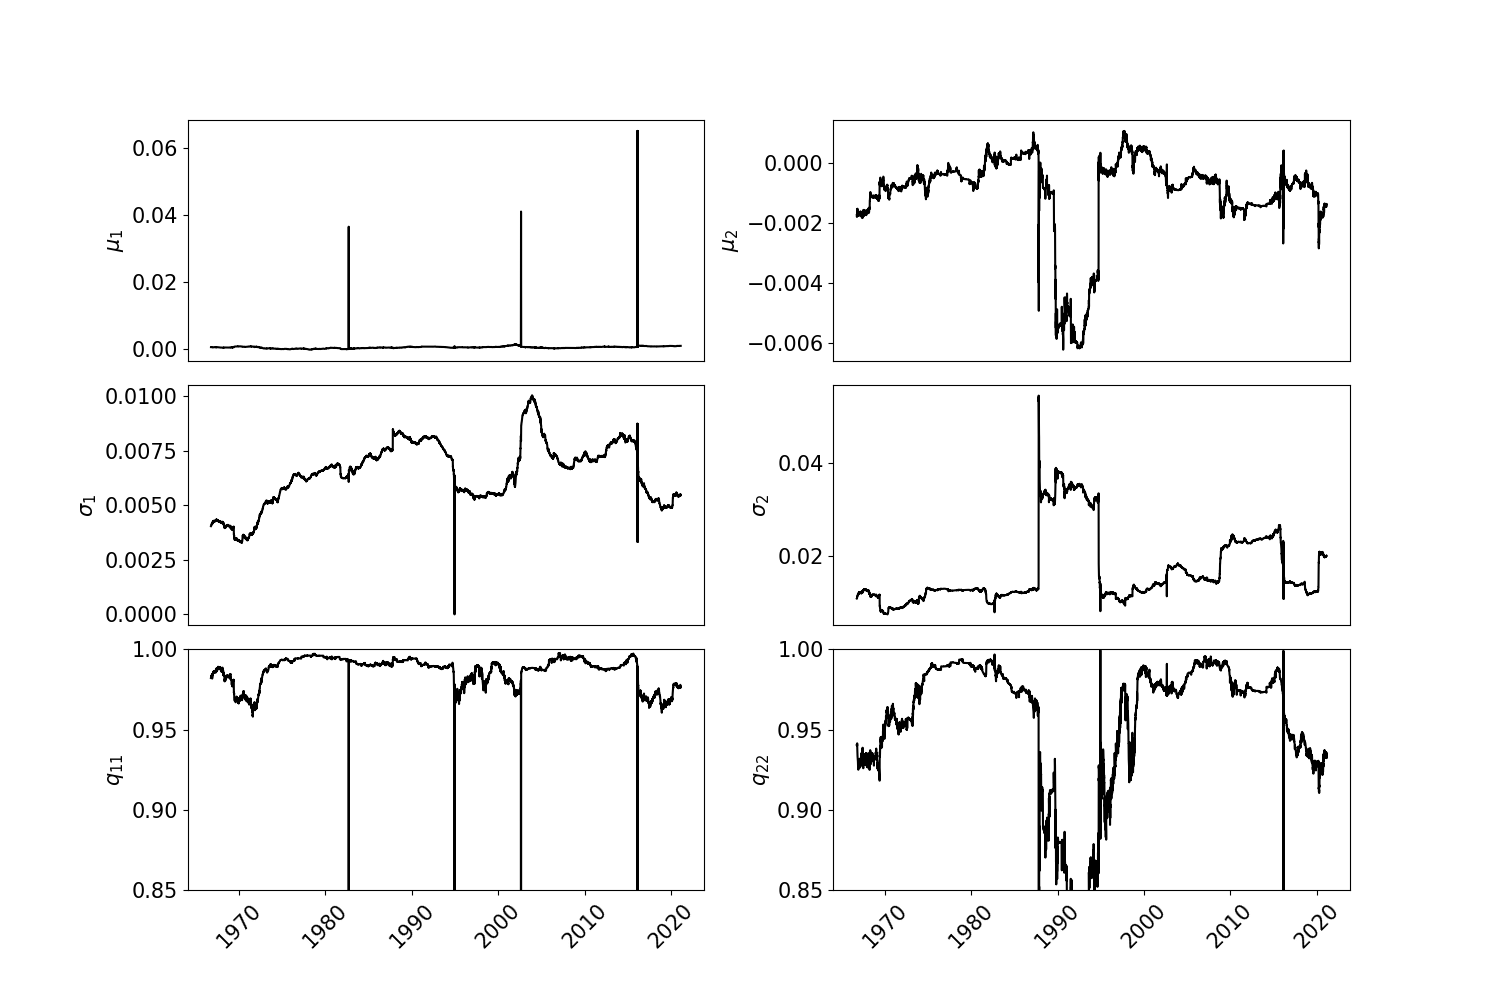
\includegraphics[width=1.0\textwidth, height=0.5\textheight]{analysis/stylized_facts/images/2-state MLE HMM rolling params.png}
    \caption[Rolling estimation based on the \mle estimator]{Rolling estimation based on the \mle estimator. The parameters are derived from a 2-state Gaussian HMM using a rolling window of 1700 days.}
    \label{fig: MLE estimation rolling parameters} 
\end{figure}

\begin{figure}[H] 
    \centering
    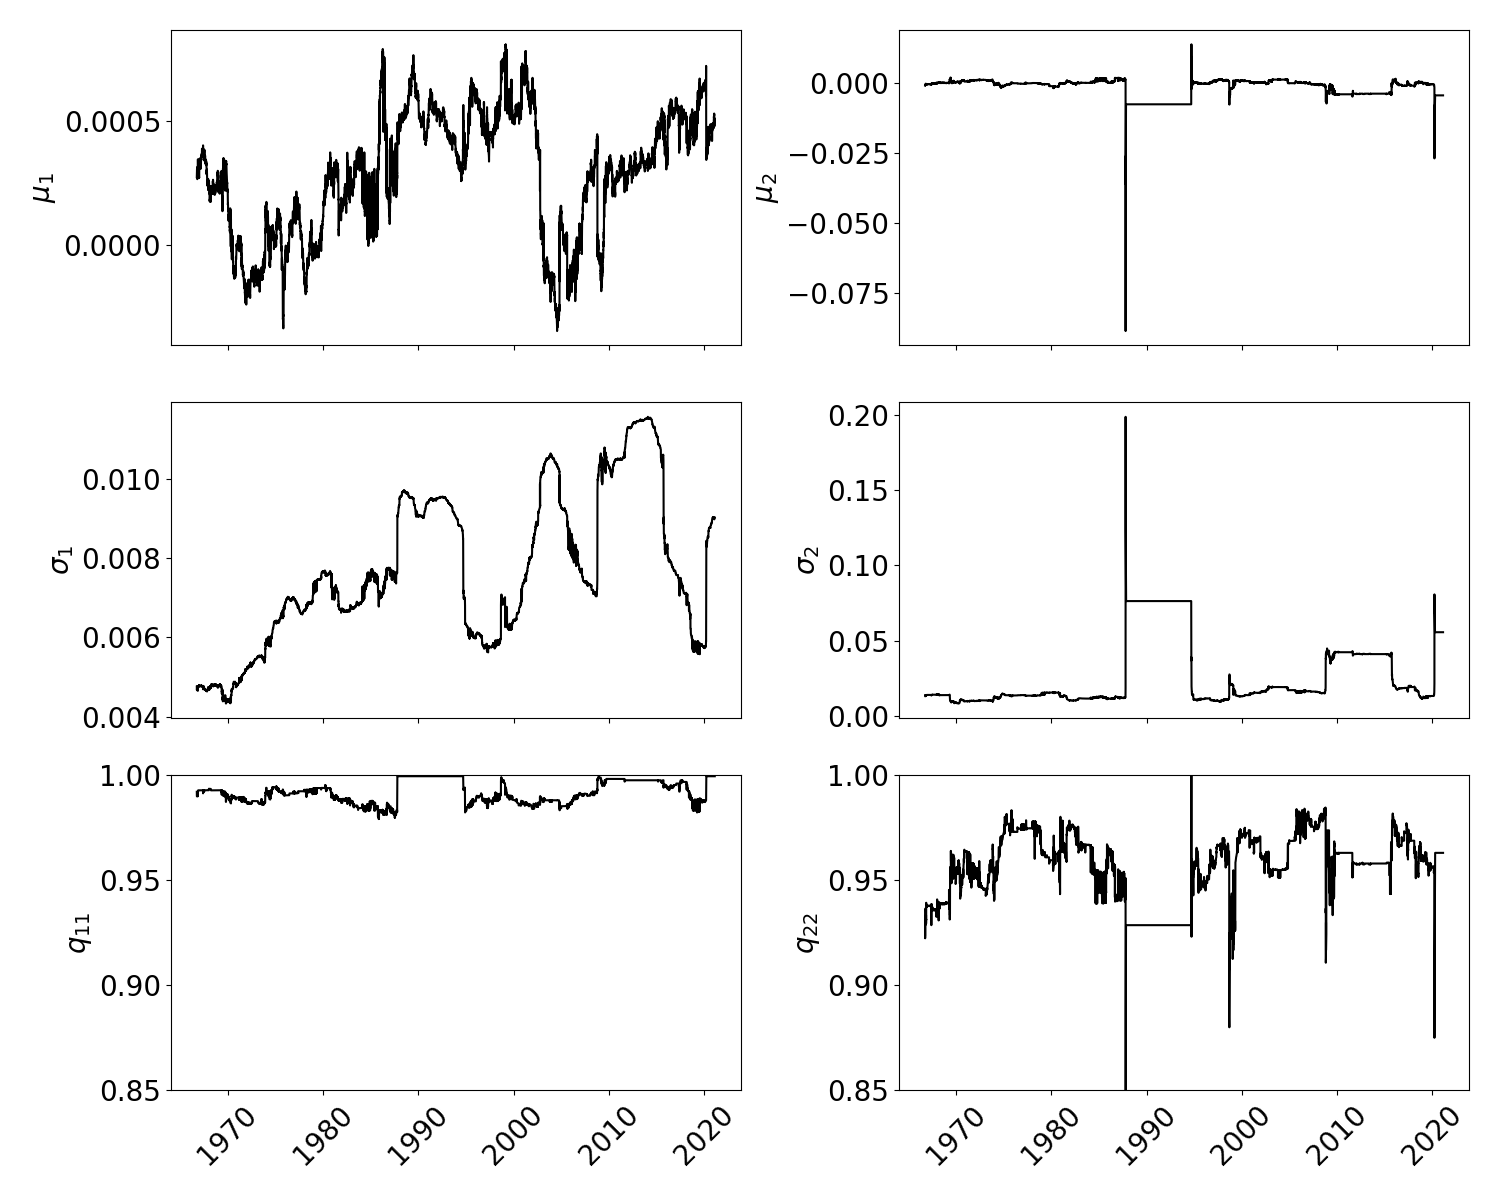
\includegraphics[width=1.0\textwidth, height=0.5\textheight]{analysis/stylized_facts/images/2-state JUMP HMM rolling params.png}
    \caption[Rolling estimation based on the \jump estimator]{Rolling estimation based on the \jump estimator. The parameters are derived from a 2-state Gaussian HMM using a rolling window of 1700 days.}
    \label{fig: Jump estimation rolling parameters} 
\end{figure}

From figure \ref{fig: MLE estimation rolling parameters} and \ref{fig: Jump estimation rolling parameters} it is evident that neither the mean nor variance parameters exhibit stationarity across time regardless of whether the estimation procedure relies on \mle or \jump approach. Starting with the \mle approach, shown in figure \ref{fig: MLE estimation rolling parameters}, the rolling window length of 1700 observations is particularly visible in the high-variance state during recessions. This is especially evident during Black Monday in 1987 and during the financial crisis in 2008 in which $\sigma_2$ spikes only to return to its old level roughly 1700 trading days later. This is an interesting behaviour because the most extreme observations from Black Monday and the financial crisis have been replaced with $\pm$ 6 times the standard deviation of the data. Yet, during these periods many other extreme returns take place and it is those observations that are responsible for the general change in $\sigma_2$. In addition, it is even more interesting that both periods of increased variance in $\sigma_2$ lies at roughly the same level. This could imply that the high-variance state fluctuates around some long term level in which large deviations only occur for extreme events such as the financial crisis and the COVID-19 recession. It could also imply the need for a third 'outlier' state with a low unconditional probability to handle these periods, but as shown by Bulla et al. (2011) such a model is often inferior to a two-state model hence it does not lead to smaller variations in the model parameters.

Interestingly, figure \ref{fig: MLE estimation rolling parameters} reveals that the mean for the first state is largely time-varying, and it has a notably large increase during the financial crisis. The same holds true for the mean in the high-variance state, especially during periods of economic turbulence, although this parameters decreases rather than increases during these dramatic periods. This development can be explained by the fact that economic history prescribe that it is highly unlikely that a large market crash is followed by an additional large market crash shortly after. As such, the model provides a good estimation for the mean in both states. When analysing the non-constant transition probabilities resulting from the \mle approach in figure \ref{fig: MLE estimation rolling parameters} it can easily be inferred that the sojourn times are mostly persistent in the low-variance state. Contrary, the transition probabilities $q_{22}$ of the high-variance state are characterised by a higher degree of fluctuations across time, mostly evident during the period following Black Monday. This means that the HMM will predict much shorter sojourn times in the high-variance state. This is a natural consequence of the properties of the transition probabilities because when $q_{22}$ decreases $q_{21}$ increases as $q_{22} + q_{21} = 1$, hence a low value of $q_{22}$ will result in more frequent transitions between states.

Moving on to figure \ref{fig: Jump estimation rolling parameters} it is evident that the \jump procedure also captures the time-varying nature of the underlying HMM parameters. The results are quite similar to those of the \mle estimator, however, the $\mu_1$ is now practically zero and the fluctuations of $\mu_2$ in the high-variance state are more abrupt during periods such as Black Monday and the financial crisis when compared to the \mle estimator. Yet, it is also evident that the high-variance state in general seem more stable with the \jump estimator in periods outside of economic turbulence. In addition, the rolling windows are also evident from the \jump approach since $\sigma_2$ spikes during Black Monday after which the parameter stabilizes at a new level, only to fall down to its original level approximately 1700 days after the event. Curiously, when analysing $\sigma_2$ the level reached during Black Monday and the financial crisis is no longer roughly equal thus rejecting the idea of two long-run levels in $\sigma_2$ when the models are estimated through the \jump framework. 

The biggest improvement of running the \jump framework as opposed to the \mle approach is seen through the estimation of the transitions probabilities for both states. Just as in the simulation study, when comparing $q_{11}$ and $q_{22}$ in figure \ref{fig: MLE estimation rolling parameters} to figure \ref{fig: Jump estimation rolling parameters} it appears that the transitions probabilities are much more stable across states when estimating the model parameters using the \jump approach. Furthermore, it appears that both model estimation procedures suggest a similar level for some of the parameters. For instance, $\sigma_1$ generally fluctuates around a level of 0.005 to 0.010 for both approaches. This provides a high degree of confidence since it is unlikely that two different estimation procedures should arrive at similar parameters randomly. Conclusively, by analysing figure \ref{fig: MLE estimation rolling parameters} and \ref{fig: Jump estimation rolling parameters} it appears that the \jump approach provides persistent transition probabilities across time, thereby suggesting that its the strongest methodology, however, further analysis of the reproduction of the stylized facts has to be conducted before this can be cemented.

Finally, figure \ref{fig:stylized_facts_rolling_moments} shows the estimated unconditional first four moments of $r_t$ as well as for the \jump and \mle estimators. As such, it is evident that both the \mle and \jump model are able to reproduce the first two moments quite well, since the mean and variance matches that of $r_t$ across all time periods.

\begin{figure}[H] 
    \centering
    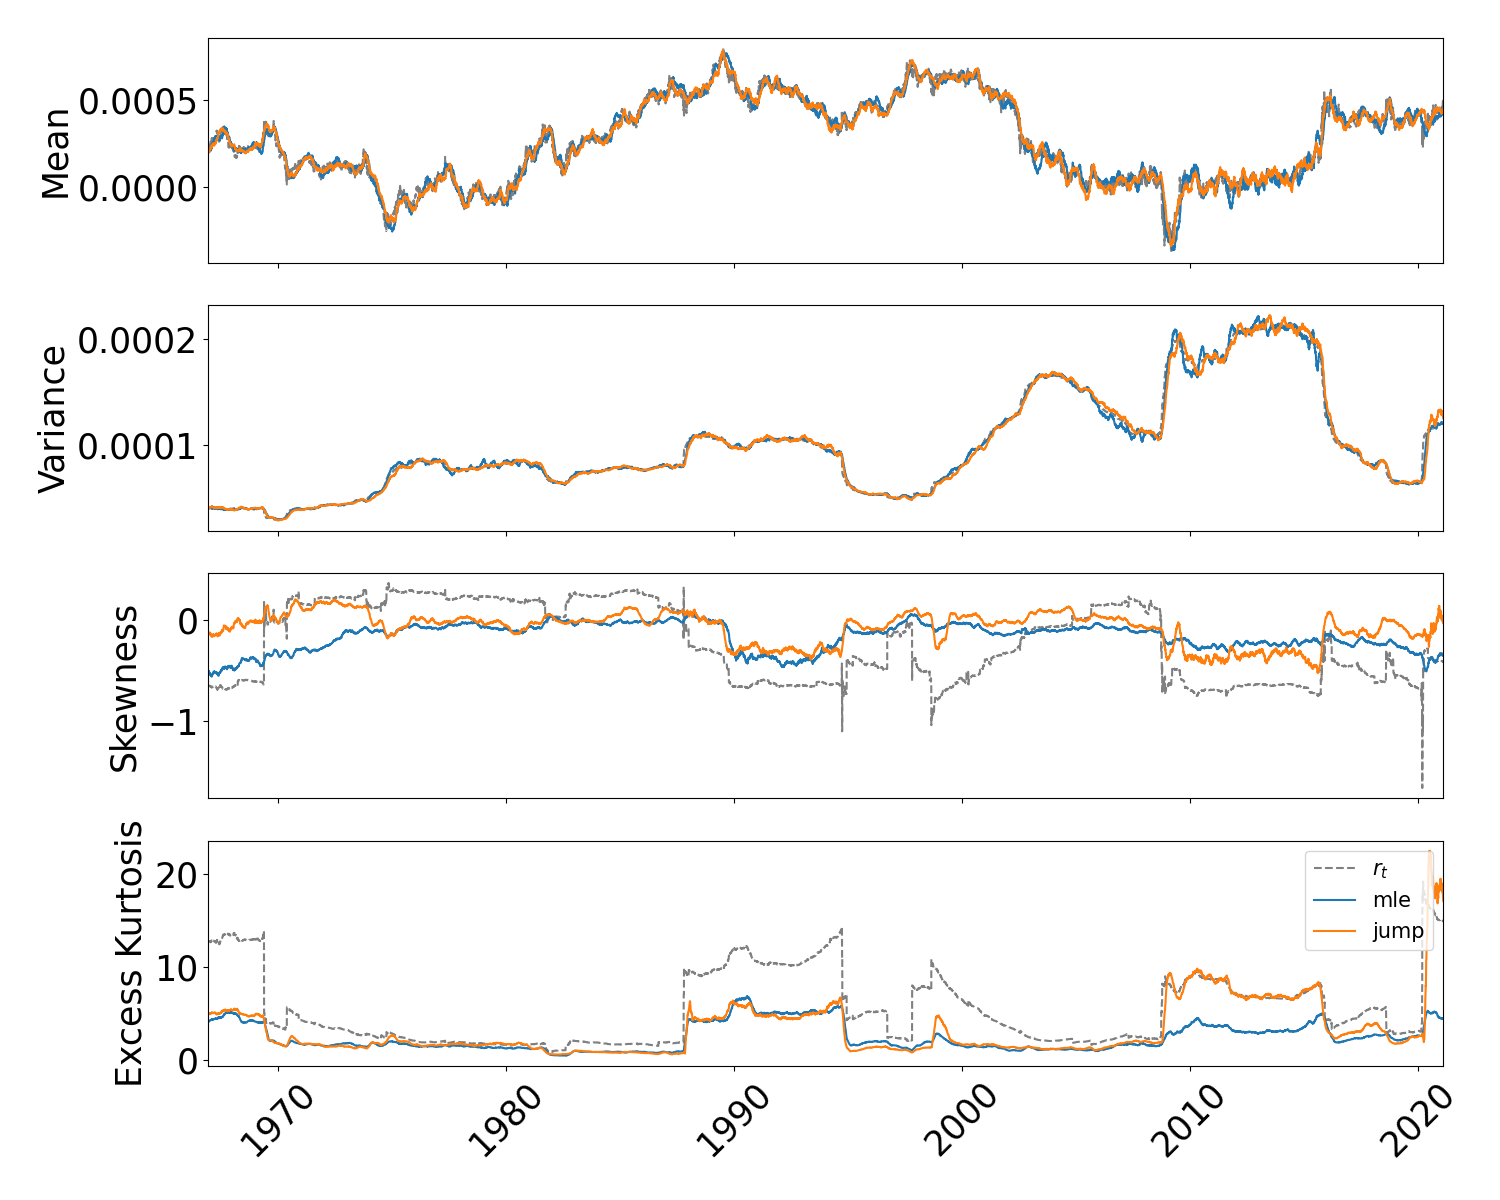
\includegraphics[width=1.0\textwidth, height = 0.4\textheight]{analysis/stylized_facts/images/moments_regular.png}
    \caption[Development of the first four moments from the estimated models and $r_t$]{Development of first four moments from the estimated models compared to $r_t$ using a rolling window of 1700 days. Model estimates are calculated using Monte-Carlo simulations.}
    \label{fig:stylized_facts_rolling_moments} 
\end{figure}

Unsurprisingly, the estimates of skewness and kurtosis are more error-prone especially during periods of economic turmoil such as during Black Monday. Still, the results are quite similar to those obtained by Bulla (2011) except that this analysis shows the full evolution of parameters over the period. When further analysing the skewness it is clear that the model parameters fluctuate around that of the data and are predominantly negative during the entire period across both models. This suggest that more observations fall into the left part of the distribution. The same conclusion is apparent for the excess kurtosis where the estimates of both models fluctuate around those of the log returns. Curiously, Bulla (2011) tended to 'overshoot' kurtosis in many of his 10 sub-samples when using t-distributions whilst blaming HMMs using Gaussian distributions for not being able to capture higher levels of kurtosis. It is then interesting to observe that apart from Black Monday, the \jump estimator is fitting kurtosis particularly well especially during the financial crisis. Additionally, the time-varying nature of the first four moments in figure \ref{fig:stylized_facts_rolling_moments} further cements the appropriateness in using rolling estimations as a static model would not have been able to capture this non-stationary data generating process.

\subsection{Reproducing the stylized facts of Granger \& Ding (1995b)}
\label{section:stylized_facts_GD}

As the parameters of the rolling models have been estimated and shown, the analysis now turns to defining the stylized facts established by Granger \& Ding (1995b) before attempting to reproduce them to uncover whether the utilized models obtain a better fit compared to Rydén et al. (1998) and Bulla (2011). The temporal and distributional properties, established by Granger \& Ding (1995b) are as follows.

\textbf{Tekst efter TPx skal indentes \newline}
TP1: Returns $r_t$ are not autocorrelated (except for, possibly, at lag 1). \newline
TP2: $|r_t|$ and $r_t^2$ are the 'long memory' i.e. their autocorrelation functions decay slowly starting from the first order autocorrelation and $corr(|r_t|, |r_{t-k}|) > corr(r_t^2, r^2_{t-k})$. The autocorrelations remain positive for many lags and the decay is much slower than the exponential rate of a typical ARMA model. \newline
TP3: The Taylor effect $corr(|r_t|, |r_{t-k}|) > corr(|r_t|^{\theta}, |r_{t-k}|^{\theta})$, $\theta \neq 1$. Autocorrelations of powers of absolute returns are highest at power one. \newline
TP4: The autocorrelations of $sign(r_t)$ are negligibly small.

The three distributional properties are as follows.

\textbf{Tekst efter DPx skal indentes \newline}
DP1: $|r_t|$ and $sign(r_t)$ are independent\newline
DP2: $|r_t|$ has the same mean and standard deviation \newline
DP3: The marginal distribution of $|r_t|$ is exponential (after outlier correction)

In addition, it should be noted that an exponentially distributed variable (DP3) $x_t$ has the following properties.

PED1: $E(x_t) = \sqrt{Var(x_t)}$ (Same as DP2) \newline
PED2: $E[x_t-E(x_t)]^3 / (Var(x_t))^{\frac{3}{2}} = 2.$ \newline
PED3: $E(x_t-E(x_t))^4 / (Var(x_t))^{2} -3 = 6.$

In the analysis conducted by Rýden et al. (1998) and Bulla et al. (2011) it has been proven that DP1 holds as a natural consequence of the construction of HMMs and that TP1 \& TP4 is not violated in practice. Since DP1, TP1 and TP4 have previously been very well reproduced the expectation is that the models presented in this thesis are able to avoid deviating too much from these stylized facts. As previously mentioned, the more difficult stylized facts to reproduce, include DP2, DP3, TP2 and TP3. Interestingly, both Ryden et al (1998) and Bulla (2011) had difficulty in reproducing these. As such, it will be the analysis of these stylized facts that are central in the coming sections starting out with the distributional properties.

\subsection{Distributional properties}
\label{Sec: Distributional properties}

In this section the analysis will focus on reproducing the distributional properties DP2 and DP3, as shown in figure \ref{fig:stylized_facts_moments_bulla_abs}, which presents the mean-standard deviation ratio, skewness and excess kurtosis of $|r_t|$ and the fitted models.

\textbf{Consider shrinking the y-axis for kurtosis.}
\begin{figure}[H] 
    \centering
    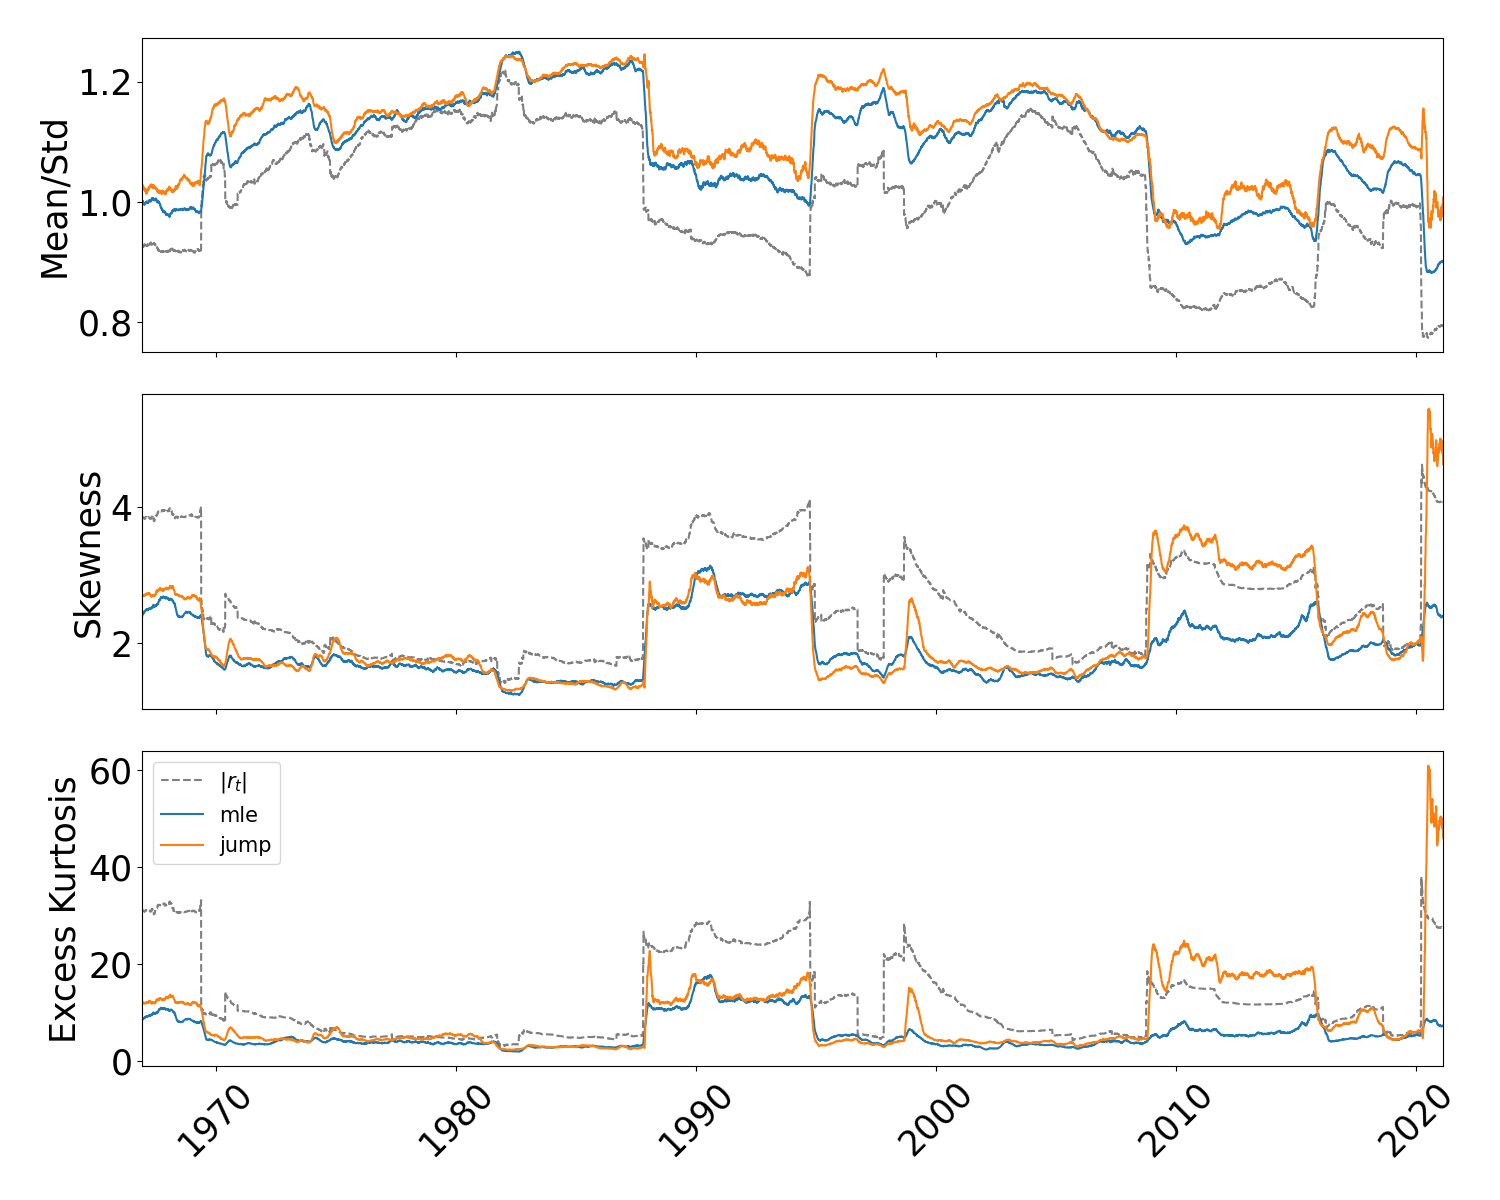
\includegraphics[width=1 \textwidth, height=0.4\textheight]{analysis/stylized_facts/images/moments_bulla_abs.png}
    \caption[$|r_t|$ and the models' distributional properties]{$|r_t|$ and the models' distributional properties. The top panel shows the mean to std ratio, the middle panel shows the skewness and the bottom panel shows the excess kurtosis.}
    \label{fig:stylized_facts_moments_bulla_abs} 
\end{figure}

When analysing the ratio of the mean and standard deviation (DP2/PED1), it can be seen that the mean is higher than the standard deviation for the predominant part of the period. This holds for both models as well as $|r_t|$ although the log returns experience a larger decline in the ratio during periods of economic turbulence. Therefore, it appears that neither of the two models sway too far away from 1, thereby indicating that the mean of the absolute returns is approximately equal to the standard deviation of the absolute returns for both models. Both the \mle and \jump models seem to fluctuate in the interval [1.0 : 1.25], which is in accordance with the findings by Rydén et al. (1998) who noted that PED1 has to be somewhat relaxed, meaning that the mean is allowed to be slightly larger than the standard deviation.

\textbf{We need a better explanation for why the models might underestimate skewness in most of the period.}

Having analysed whether the models satisfy PED1 and DP2 the final distributional property to consider is PED2 and PED3 in DP3. This is due to the fact that in order for DP3 to be satisfied the models must exhibit the properties of PED1, PED2 as well as PED3 simultaneously. Since it was just shown that DP2 holds for both models, and PED1 and DP2 are identical in their construction, it can be concluded that PED1 holds for both models. Moving on to PED2 it is evident that both the \mle and \jump model underestimate skewness in most of the period, however, it appears that the \jump model achieves a much better fit of skewness in the period following the financial crisis of 2008. Interestingly, it is clear from figure \ref{fig:stylized_facts_moments_bulla_abs} that the \mle model better matches the skewness property of PED2 (i.e. that it equals 2) compared to not only the \jump model but also the data $|r_t|$ itself. It should be noted though, that the original DP3, and thus PED2, by Granger \& Ding (1995b) only hold for outlier corrected data, for which the property generally seem to hold for both models and log returns as shown in figure \ref{fig:stylized_facts_moments_bulla_abs_outliers}. This will be analyzed further in the end of this section. 

Furthermore, it is evident that both models seem to underestimate the skewness of the empirical data $|r_t|$ particularly during the period following Black Monday as well as the extraordinary bull-market leading up to the dot-com bubble. As such, the finding is a testament to the on-going issue in which even advanced models are unable to capture the full extent of the fat tails in distributions of financial returns. This finding is further backed by the fact that it appears that both models are able to reproduce the skewness in non-volatile market periods, however, the errors arrive when the rolling model contains observations from turbulent market periods. Despite this, it appears that both models are able to capture the changing skewness and excess kurtosis around the time of large market movements. This is evident throughout the figure, but particularly around the time of the GFC. The fact that both models are able to do so is particularly promising as it provides substantial evidence towards the adequacy of the models. The fit of the models could be further improved by increasing the number of states, however, the problem with such an option is that it significantly increases the risk of overfitting (Bulla 2011). As such, it can be concluded that both models somewhat reproduce PED2.

The final property that the models must satisfy in order for DP3 to be met is PED3. As such, the models must be able to exhibit and match an excess kurtosis of 6. It is clear from figure \ref{fig:stylized_facts_moments_bulla_abs} that the \mle model slightly underestimates the excess kurtosis for the predominant period of time, however, similar to the observations of the skewness, the model approximately matches an excess kurtosis of 6 in most of the period, since its average over the period is 5.51. The \jump model, however, fluctuates around the kurtosis of $|r_t|$ with it being smaller during the period following Black Monday, slightly larger during GFC and much larger during the Covid-19 outbreak. This is in line with the \jump model's slightly larger fluctuation in its parameter estimates of $\mu_2$ and $\sigma_2$ during these periods compared to the \mle model. This is quite a satisfactory results as both Rydén et al. (1998) and Bulla (2011) underestimated kurtosis of Gaussian HMMs throughout their studied time periods.

To summarize the findings above it is clear that both the \mle and the \jump models are able to somewhat reproduce the properties of PED1 to PED3, hence it can be concluded that DP3 approximately holds. This is similar to the conclusion reached by both Rydén et al (1998) and Bulla (2011), although they only tested HMMs estimated through the \mle methodology. As such, this section contributes to the quantitative finance literature by showcasing that the stylized facts introduced by Granger \& Ding (1995b) can in fact also be somewhat reproduced by a \jump model. As such, the thesis has extended on the introduction of \jump estimation procedure for HMMs by Bemporad el at. (2018) by proving that it matches the properties of the stylized facts associated with returns on financial assets.

\subsubsection{Outlier-corrected data}

As a final remark on the distributional properties, outlier corrected data limited to the boundary of the closed interval $[\bar r_t - 4\hat\sigma, \bar r_t + 4\hat\sigma]$ will be subject to analysis. As noted by Granger \& Ding (1995b), DP3 was found to only hold on outlier corrected data and even though the above findings were somewhat satisfactory, the analysis is repeated for outlier corrected data. The results are shown in figure \ref{fig:stylized_facts_moments_bulla_abs_outliers}. It can be concluded from the figure that the results are similar to those of Bulla (2011), since he did not find large changes between the full data and the outlier corrected data in regards to whether the models reproduce the distributional properties. The mean to standard deviation ratio has risen in magnitude, but the shapes remain largely unchanged. The same conclusion holds for skewness and kurtosis. As a result, the major difference is simply that results have shifted towards the values of an exponential distribution (PED1-3), but the shapes of the curvatures remain rather unchanged.

\textbf{Begge modeller er her meget tættere på $|r_t|$ end for ikke outlier-corrected data. Men det er kun fordi momenterne har taget et lodret skift ned. Spørgsmålet er om outlier-corrected data vil give bedre density forecasts i den efterfølgende porteføljeøvelse?}

\begin{figure}[H] 
    \centering
    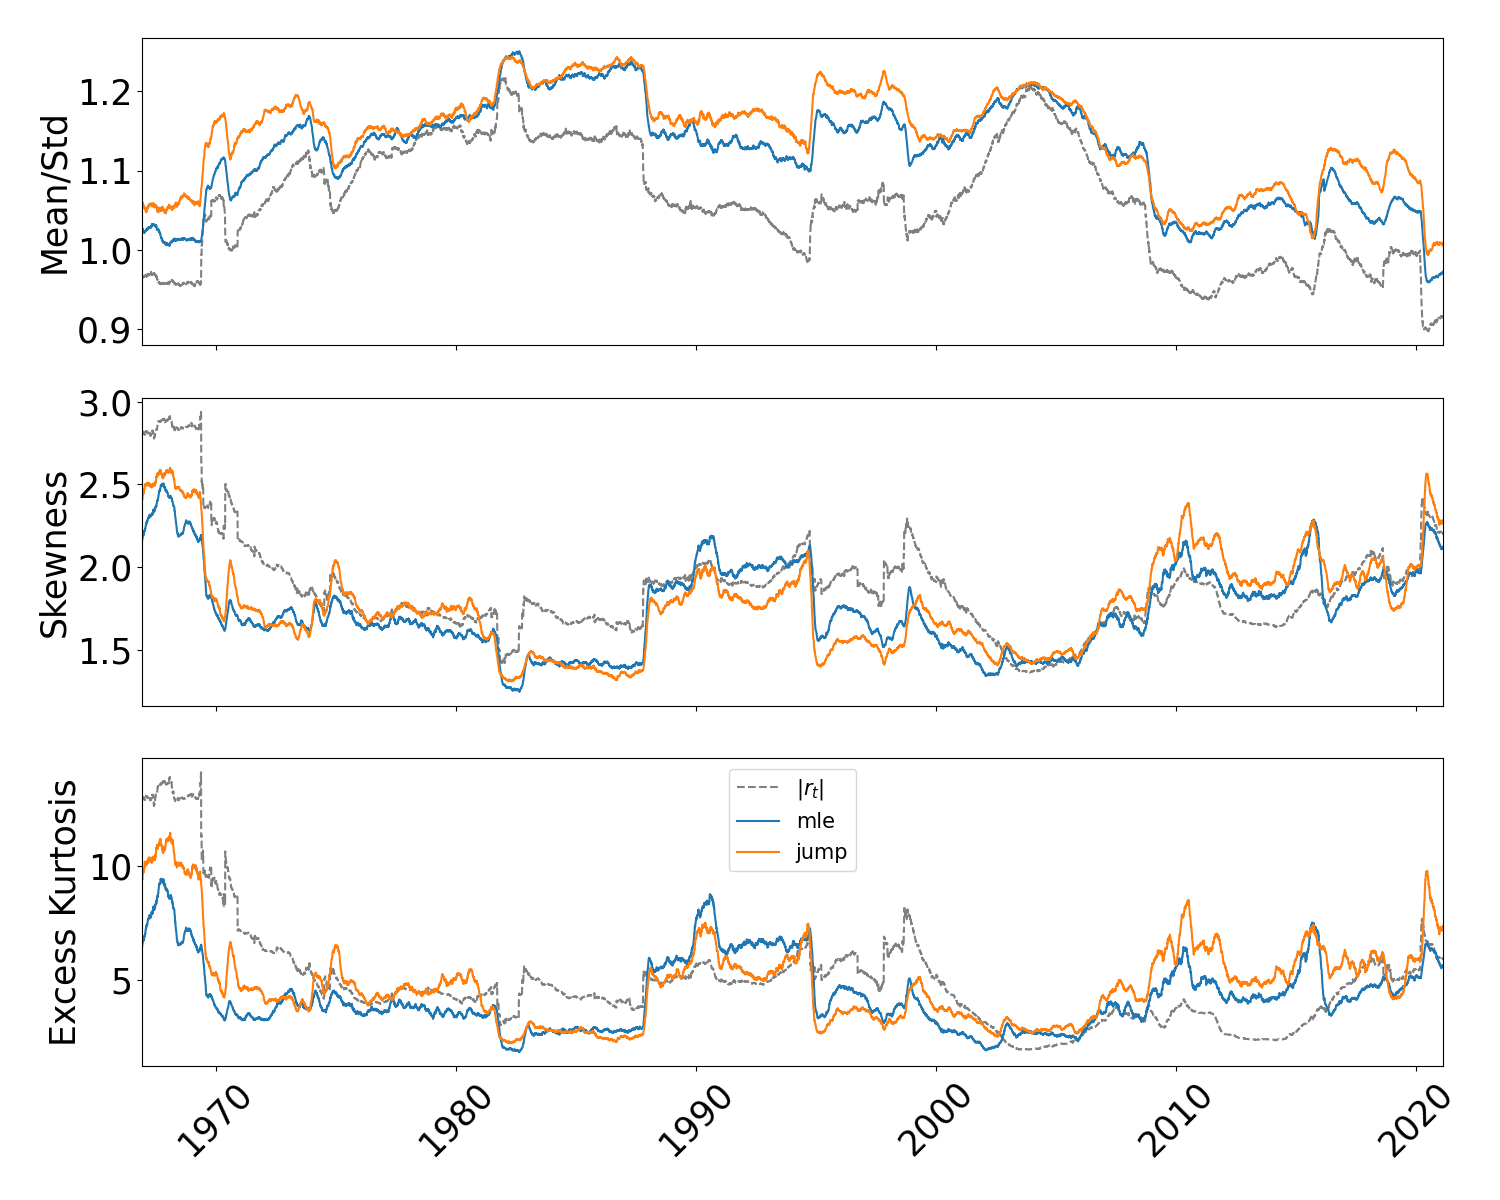
\includegraphics[width=1.0\textwidth, height = 0.4\textheight]{analysis/stylized_facts/images/moments_bulla_abs_outlier.png}
    \caption[$|r_t|$ and the models' outlier corrected distributional properties]{$|r_t|$ and the models' outlier corrected distributional properties. The top panel shows the mean to std ratio, the middle panel shows the skewness and the bottom panel shows the excess kurtosis. \textbf{Consider moving to appendix}}
    \label{fig:stylized_facts_moments_bulla_abs_outliers} 
\end{figure}

\subsection{Temporal properties}
\label{Sec: Temporal properties}

Having analyzed the distributional properties, the next logical step is to check the temporal properties as defined by Granger \& Ding (1995b). As mentioned earlier, previous research suggest that HMMs are able to reproduce most of the stylized facts quite well, however, Rydén et al. (1998) and Bulla (2011) found that HMMs are inadequate when it comes to reproducing the slow decay of the autocorrelation function of absolute daily returns which is often referred to as volatility clustering. Rydén et al (1998) considered this the most difficult stylized fact to reproduce for HMMs.

As such, most of this section will be dedicated to reproducing TP2, however, TP3 will also be covered. TP1 and TP4 are shown in appendix \ref{appendix:sign_rt}. The section is structured as follows. Initially, the authors provide some initial thoughts into why both Rydén et al. (1998) and Bulla (2011) might have had difficulty in reproducing the slow decay in the absolute autocorrelation function. The analysis then proceeds to show how the rolling models have a much slower decay in their absolute autocorrelation functions when compared to the models of Rydén et al. (1998) and Bulla (2011). Secondly, TP3 is sought reproduced by the \mle and \jump models and finally the analysis will briefly show that TP1 and TP4 are not violated.

\subsubsection{Preliminary thoughts on the ACF in static versus rolling models}

This section provides some insights into the differences for the autocorrelation function when it is derived from the full sample compared to several sub-samples. This is used to further motivate the use of rolling models. Figure \ref{fig:stylized_facts_acf_data} shows the autocorrelation of $|r_t|$ on the full sample as well as the average autocorrelation of sub-samples each containing 1700 observations. It is evident from the figure that the decay is more exponential for the sub-samples and by lag 200 the absolute autocorrelation is practically insignificant wheres the absolute autocorrelation for the full sample remains significant until lag 430, thereby exhibiting a slower decay. The faster decay in the sub-samples is most likely a result of the periods without excess risk and economic turmoil. These periods cause very low estimates of the ACF, as the volatility clustering is less significant in these periods, thereby increasing the speed of the decay. In any case, it is clear that the 'long-memory' effect has decreased in the bottom panel of figure \ref{fig:stylized_facts_acf_data}.

\begin{figure}[H] 
    \centering
    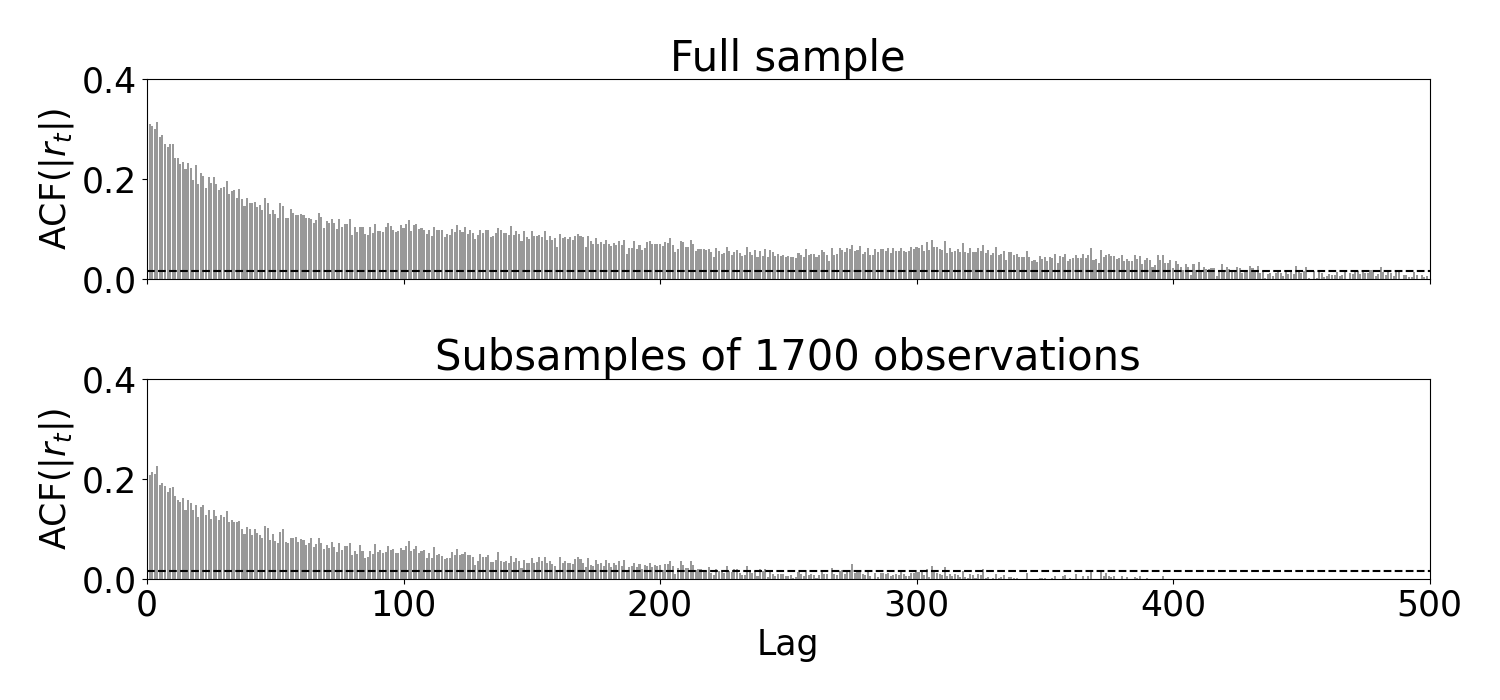
\includegraphics[width=1.0\textwidth]{analysis/stylized_facts/images/acf_data.png}
    \caption[Autocorrelation function of $|r_t|$ on full sample and subsamples]{Autocorrelation function of $|r_t|$. The top panel shows the ACF estimated on the full sample and the bottom panel shows the average ACF when the data is split into rolling subperiods of 1700 observations.}
    \label{fig:stylized_facts_acf_data} 
\end{figure}

This finding should already make one suspicious of estimating static models in a few sub-periods as Rydén et al. (1998) and Bulla (2011) did. To show the performance of the models in such a setup the procedure by Rydén et al. (1998) and Bulla (2011) is repeated. The results are shown in figure \ref{fig:stylized_facts_acf_plots_sub_periods}. As already mentioned, it is evident that there exists clear differences in the level of ACF between the sub-periods, with some periods exhibiting quite high levels of autocorrelation and other periods in which it dies down within 50 lags. The performance of both the \mle and \jump model is roughly as reported by Bulla (2011), in which the decay is generally much faster for the models than for the log returns. One interesting finding is that the \mle model appears to fit the empirical autocorrelation quite well in sub-period 3 and 8, which are periods of turmoil. Having shown how the models would have performed in a static scenario, the same analysis will now be conducted for the rolling model.

\begin{figure}[H] 
    \centering
    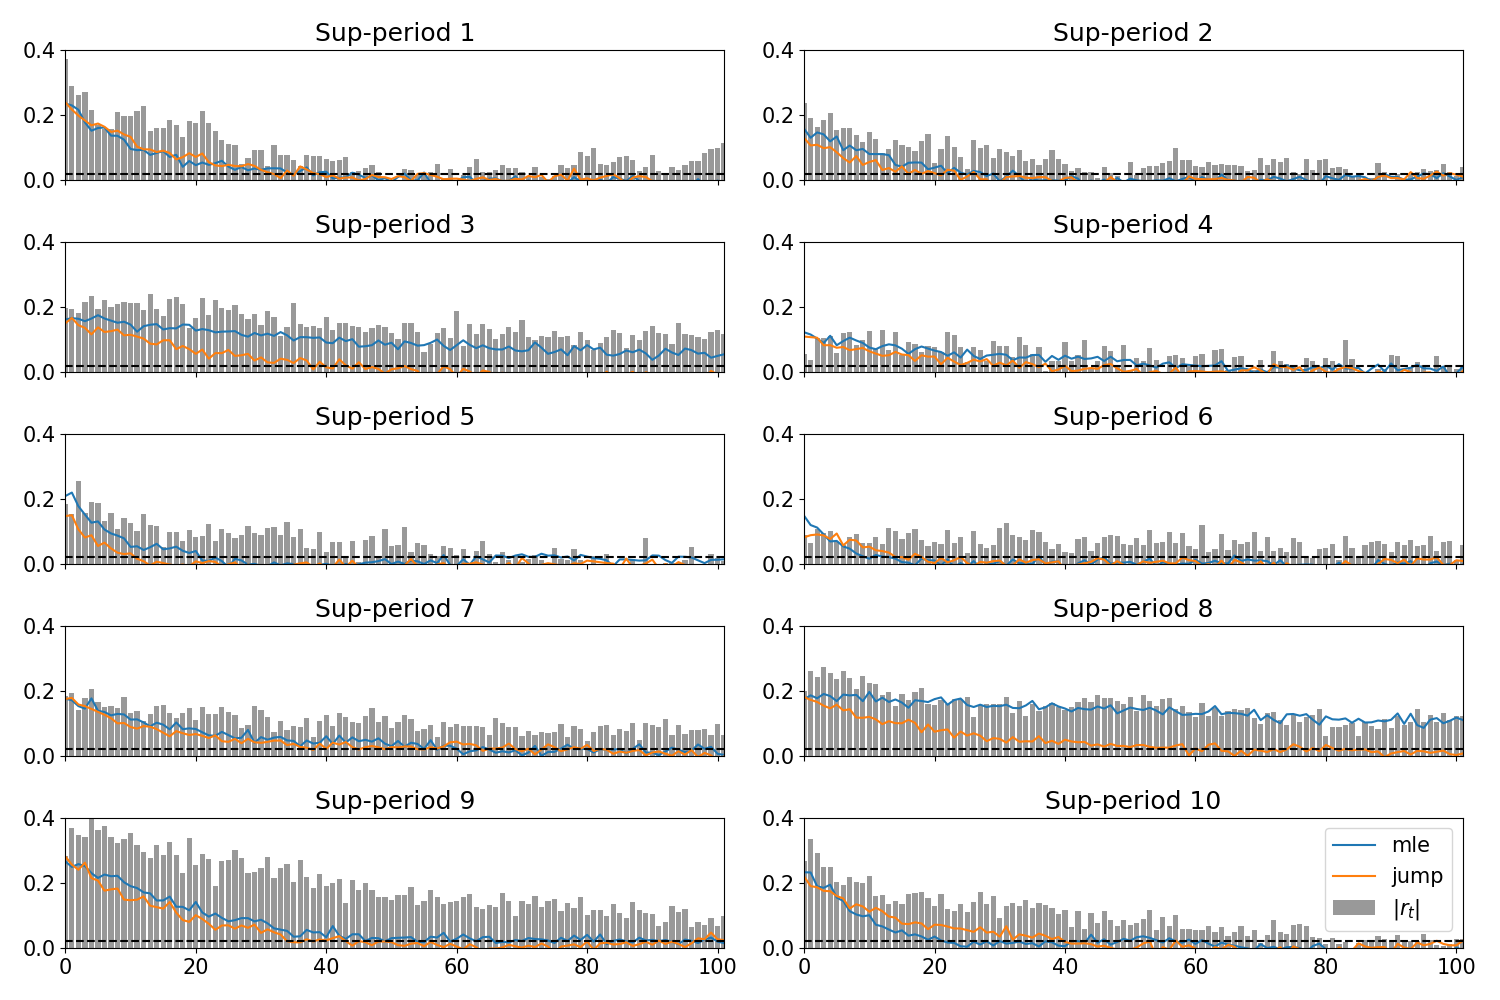
\includegraphics[width=1.0\textwidth]{analysis/stylized_facts/images/acf_abs_subperiods.png}
    \caption[Autocorrelation function of estimated models and $|r_t|$ on subsamples]{Autocorrelation function of estimated models and $|r_t|$ in a breakdown of 10 subperiods each of 1700 observations. Results are similar to those of Ryden et al. (1998) and Bulla (2011). In most periods the ACF is underestimated and both models' ACF becomes insignificant within 50 lags. \textbf{Ret stavefejl i Sub-period.}}
    \label{fig:stylized_facts_acf_plots_sub_periods} 
\end{figure}

\subsubsection{Temporal properties of the rolling model}

In order to get an overview of the full sample period, figure \ref{fig:stylized_facts_acf_plots} plots the full sample empirical absolute autocorrelation function together with the simulated absolute ACF functions of the \mle and \jump models. The black dashed line is the upper boundary of the 95\% confidence interval under the null hypothesis of independence (Madsen, 2008). The absolute autocorrelations of both the \mle and \jump model have significantly increased and is now larger than that of the data at lags above 350. Interestingly, the initial decay of both models is stronger than $|r_t|$ for the first $\sim$ 50 lags after which it flattens out.\textbf{Think about a good reason for why this might be.}
The reader should note that the persistence of the ACF of the absolute returns is, to some extent, a consequence of the aforementioned volatility clustering and the significance of the lags above lag 100 is more likely a result of the data-generating process being non-stationary as mentioned earlier. 

\begin{figure}[H] 
    \centering
    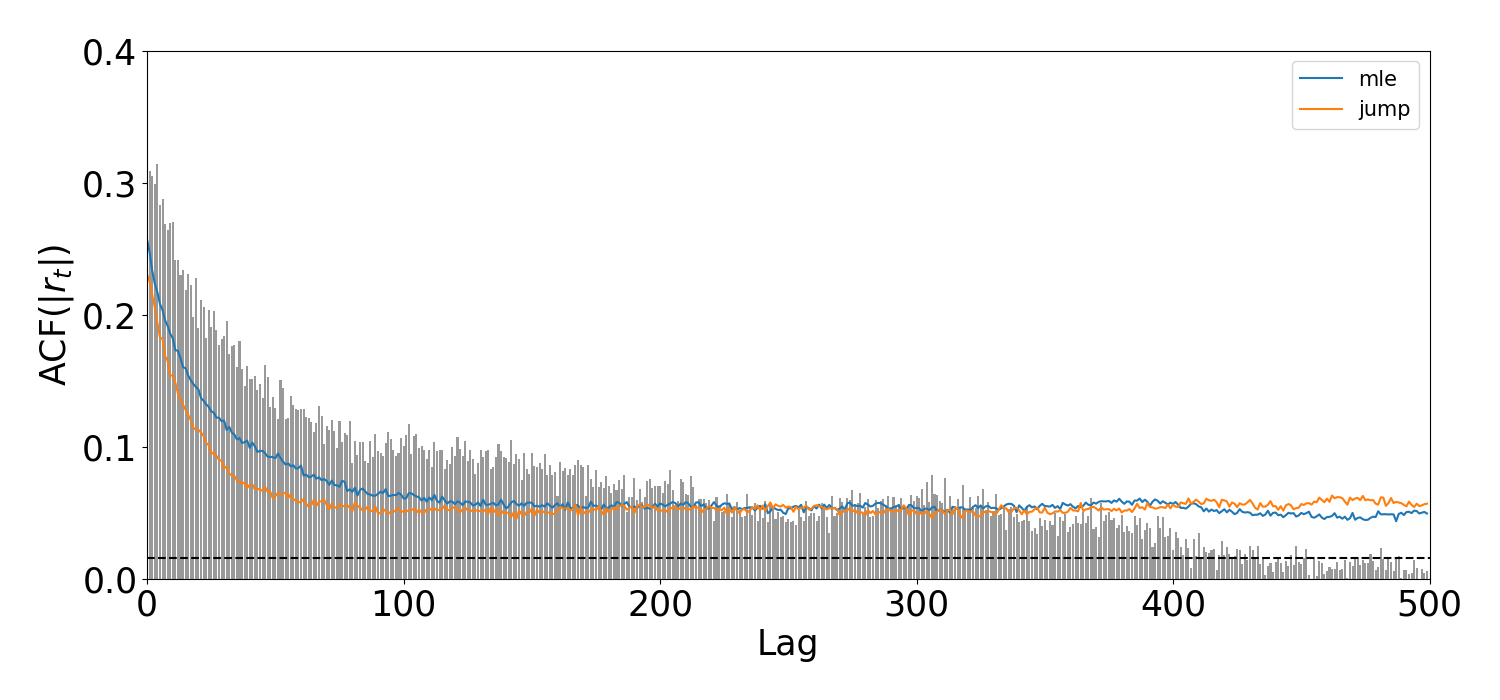
\includegraphics[width=1.0\textwidth]{analysis/stylized_facts/images/acf_abs.png}
    \caption[Autocorrelation function of estimated models as well as $|r_t|$ on full sample data]{Autocorrelation function of estimated models as well as $|r_t|$ on full sample data.}
    \label{fig:stylized_facts_acf_plots} 
\end{figure}

From the plot in figure \ref{fig:stylized_facts_acf_plots} it is also evident that the \mle model does a better job at reproducing the shape of the absolute ACF for the first 200 lags, however, the performance of the models is similar after this point. In addition, neither of the models' absolute autocorrelation become insignificant even at very large lags which is in line with the actual autocorrelation of the absolute empirical returns. The reader should note that since the computation underpinning the autocorrelation plots of figure \ref{fig:stylized_facts_acf_plots} relies on simulations, the true absolute autocorrelations are probably higher as the bouncing behaviour from the simulations exhibited in figure \ref{fig:stylized_facts_moments_bulla_abs_outliers} should reduce autocorrelation.

The remaining stylized fact is TP3, i.e. $corr(|r_t|, |r_{t-k}|) > corr(|r_t|^{\theta}, |r_{t-k}|^{\theta}) \forall \theta \neq 0$, which is often referred to as the Taylor effect. In order to analyse whether the Taylor effect holds the coefficient $\theta$ is estimated for every period by maximizing the first order autocorrelation of $|r_t|^{\theta}$. As with Rydén et al. (1998), the computation is conducted through Monte-Carlo simulations and subsequent numerical maximization. Figure \ref{fig:stylized_facts_taylor_effect} summarizes the results.

\begin{figure}[H] 
    \centering
    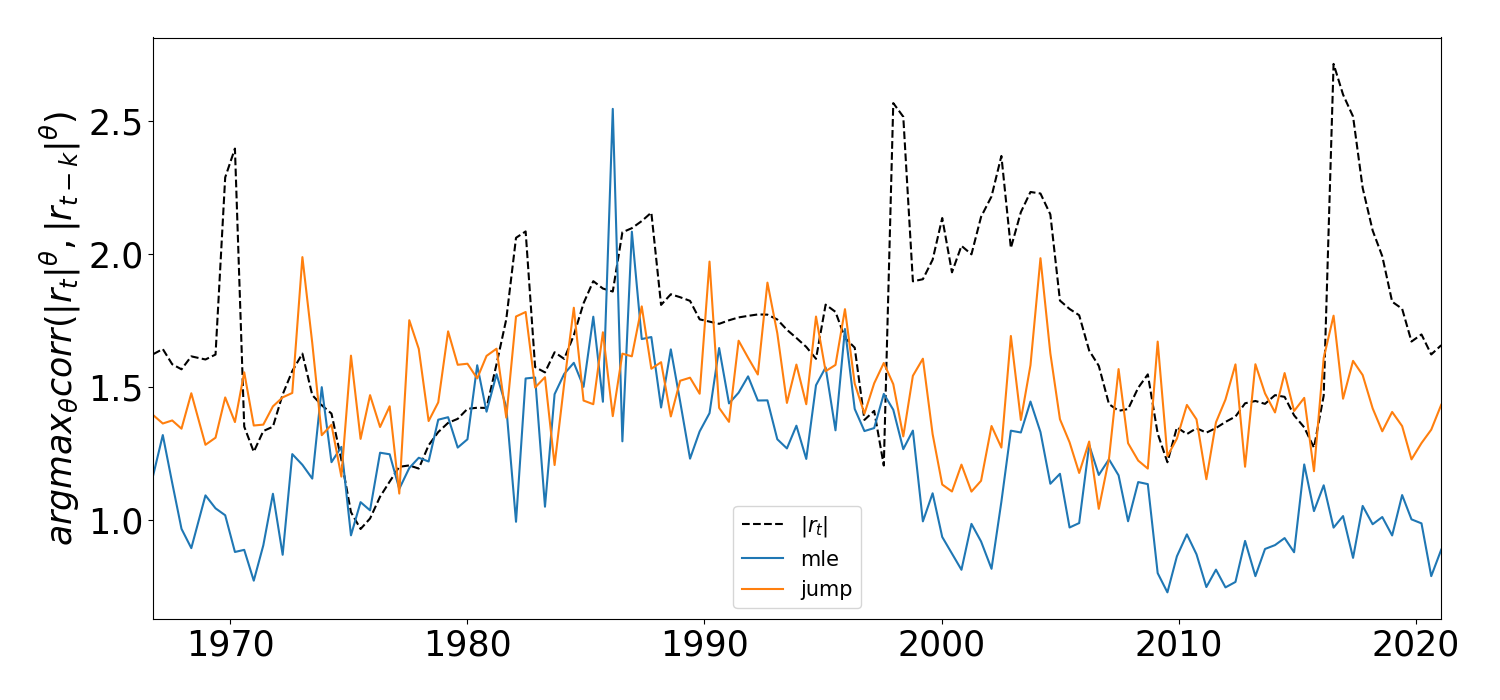
\includegraphics[width=1.0\textwidth]{analysis/stylized_facts/images/taylor_effect.png}
    \caption[Taylor effect comparison of the $\theta$ maximizing first order autocorrelations of $|r_t|^{\theta}$ and for the models]{Taylor effect comparison of the $\theta$ maximizing first order autocorrelations of $|r_t|^{\theta}$ and for the models. It is computed by Monte-Carlo simulations and subsequent use of numerical maximization.}
    \label{fig:stylized_facts_taylor_effect} 
\end{figure}

It is evident that the maximizing values of $\theta$ for the data series are not exactly equal to 1, thereby suggesting that neither models fully capture the properties stipulated by TP3. Even so, the fluctuation of both models is roughly the same as that observed by $|r_t|$, although the data fluctuates more aggressively. Apart from a smaller period from 1998 to 2005, the general direction of both models appears to follow that of the data, thereby indicating model adequacy.

\subsection{Decoding and prediction}

\textbf{This section is currently not really used for anything except showing pretty graphs as state prediction is not used in the asset allocation strategies. Should be changed to either focus on the posterior probabilities in each state, since this is used in forecasting, or something else. Otherwise delete.}

\textbf{Should be centered around 1-step density forecasts or the persistence of states in a rolling model.}

\textbf{Test if state persistence is improved on outlier-corrected data --> This can easily be done in an out-of-sample setting.}

As mentioned in section \ref{section: estimation} the hidden states are uncovered through the Viterbi algorithm. Since the estimation procedure is based on a rolling window, the state at time $t$ is estimated by using the most recent observation as well as the previous 1699. As such, the decoding procedure iterates through the entire row of observations 1 time step at a time as shown in figure \ref{fig:stylized_facts_decoded_states}. As previously mentioned, it is important to stress that the objective of this procedure is not to predict future states of the economy, but rather to identify and uncover the current state underlying the economy given past observations. 

\begin{figure}[H] 
    \centering
    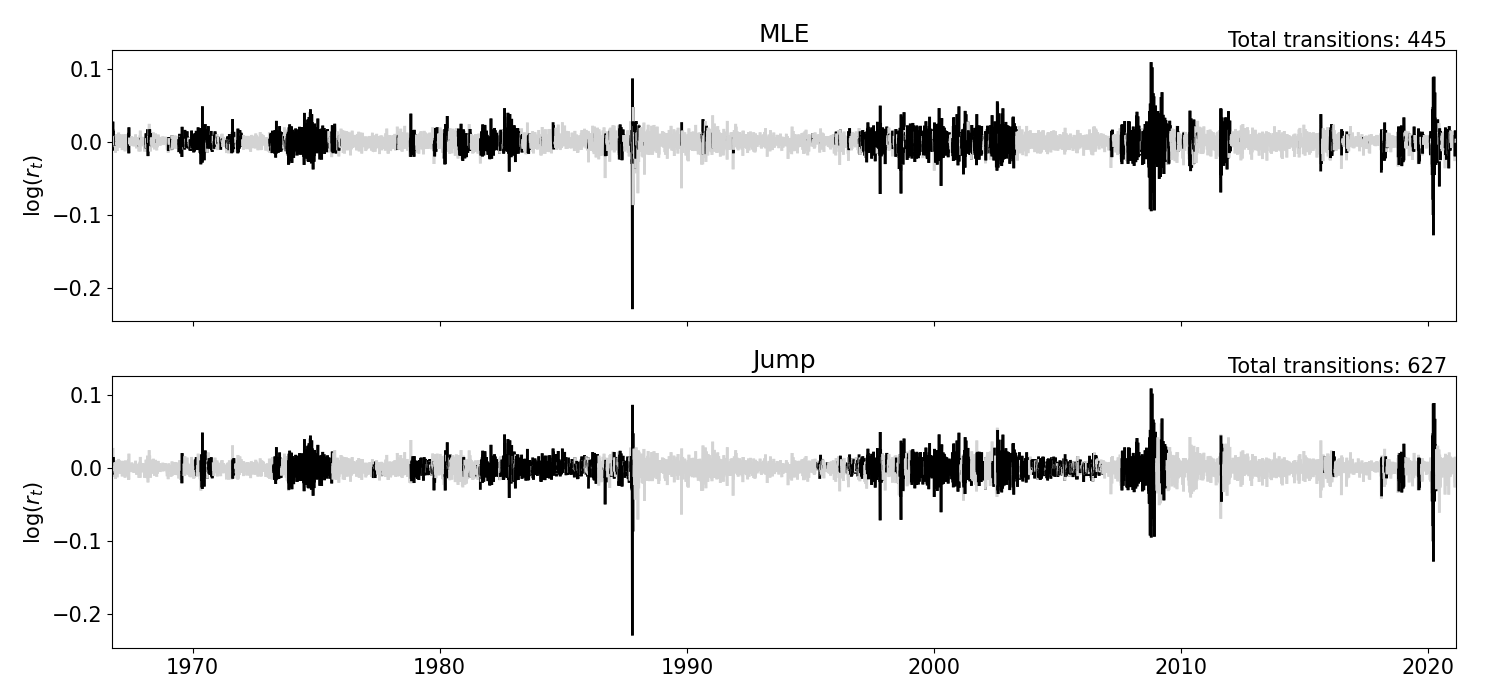
\includegraphics[width=1.0\textwidth]{analysis/stylized_facts/images/decoded_states.png}
    \caption[S\&P 500 $\log r_t$ plotted with the respective models' decoded states]{S\&P 500 $\log r_t$ plotted with the respective models' decoded states. States are decoded using a rolling window of 1700 trading days. Black indicates the high-variance state. \textbf{Fjern black monday etc. fra plot}}
    \label{fig:stylized_facts_decoded_states} 
\end{figure}

It is evident from the figure that the \mle model does a decent job in detecting the high-volatility states. However, it also appears that the model identifies some high-variance states in periods characterised by low market volatility, for instance in the beginning of the 1990s. This is most likely a result of low excess kurtosis. A similar pattern appears when analysing the decoding states of the \jump model since it too does a fairly good job at identifying the high-variance state, although the two methods disagrees in some time periods. This is for instance evident when looking at 1985 to 1990 where the \mle models suggests a low variance state, contrary to the \jump model. Furthermore, it appears that the \jump model is less consistent compared to the \mle model as it jumps around more sporadically. This is backed by the fact that the \jump model suggests 627 state transitions throughout the period which is more than 40\% more state changes compared to the suggested 445 transitions by the \mle model. This is perhaps surprisingly since the \jump framework penalizes state transitions, however, this is most likely a result of the rolling estimation approach. As such, if one were to conduct a similar analysis in which the \jump model was estimated by batches or on the full sample size, the total suggested transitions would most likely decrease, albeit these estimation procedures would introduce other problems. 

In addition, it is positive to witness that both models correctly identifies major market events such as Black monday in 1987, the dot-com bubble of the early 2000s, the GFC of 2008 and most recently the COVID-19 recession as high-variance states, albeit the models disagree in terms of how long the high-variance state persists. Furthermore, it was evident by figure \ref{fig: SP500_index} that there were short periods of large positive returns following the big market crash in September/October 2008, however, both models predict those as bear states, which indicates that variance dominates means in the prediction of whether a state is classified as high or low variance. Another aspect that has to be considered in terms of using the either model, but particularly the \jump, is the cost of changing the portfolio allocation due to a wrong signal. As evident by figure \ref{fig: SP500_index} the period from 1980 to 1990 is characterised by increasing price levels and low variance, hence the correct classification of the state should be low-variance, however, the \jump model classifies it as a high-variance state throughout the period. As such, utilising the models when forming DAA strategies should be done carefully, as the amount of transitions and possibly miss-specified states can decrease profits and Sharpe ratios substantially.  

\subsubsection{Smoothing}

\textbf{TBD. Dette afsnit har ingen værdi da vi bruger densities i forecasts - et medianfilter kan ikke implementeres i mpc approachen.}

In the previous section it became evident that the amount of transitions between the two states are high for both models with the \mle and \jump model proposing 445 and 627 transitions respectively. This amount of state transitions decreases the confidence that the uncovered state changes occur due to the economy entering a new state, while increasing the suspicion towards random sporadic jumps. Furthermore, it was evident that the \jump model proposed more than 40\% more transitions compared to the \mle, and this constitutes an issue due to the objective of \jump model being to constrain sporadic and frequent jumps. Lastly, such fluctuations and sporadic transitions can be costly in a DAA framework, especially when factoring in opportunity cost of allocating capital poorly due to a miss-specified state, and when factoring in actual trading costs. As a result of these conclusions, a probability smoothing scheme is implemented to improve persistence and hence reduce the amount of state transitions. For every state prediction at time $t$, the probability of being in all states are computed as described in section \ref{section: estimation}. This is then compared to a median threshold hence a state change will only occur if the past 4 out of 7 state predictions suggest that a change must occur. The choice of threshold is a trade-off between the time-delay in state changes and the confidence in state predictions as described by Nystrup (2014). The associated results of applying such a smoothing scheme is shown for the \mle and \jump model in figure \ref{fig:stylized_facts_decoded_states_filtered}.

\begin{figure}[H] 
    \centering
    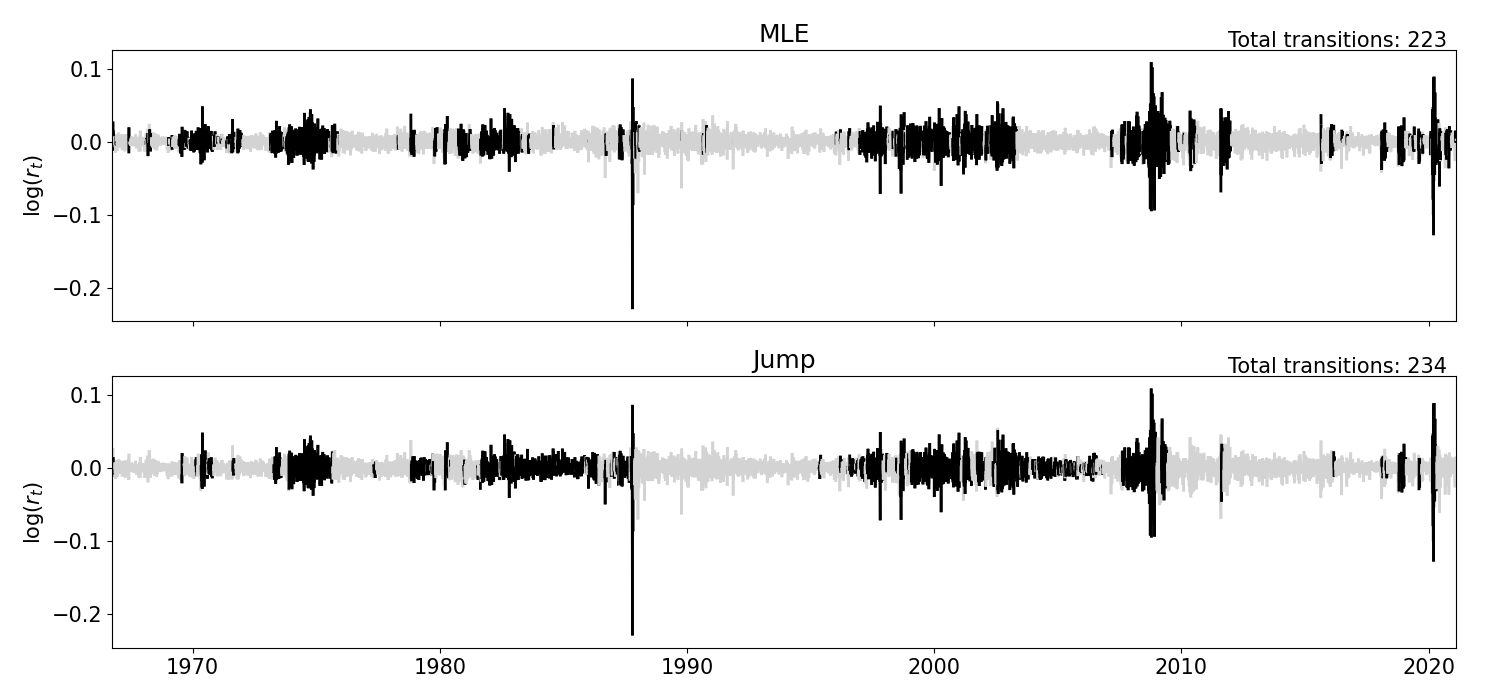
\includegraphics[width=1.0\textwidth]{analysis/stylized_facts/images/decoded_states_filter.png}
    \caption[S\&P 500 $\log r_t$ plotted with the respective models' smoothed decoded states]{S\&P 500 $\log r_t$ plotted with the respective models' smoothed decoded states. States are decoded using a rolling window of 1700 trading days.  Black indicates the high-variance state.}
    \label{fig:stylized_facts_decoded_states_filtered} 
\end{figure}

It is evident that the number of proposed transitions reduces dramatically from 445 to 223 for the \mle model and from 627 to 234 for the \jump model. The drastic decrease in transitions is primarily visible in the fewer amount of short-lived sojourn times. However, despite the apparent decrease in the number of transitions, there still appears to be inconsistency across the two models in terms of state predictions. This is once again evident in the time period from 1985 to 1990 in which the \mle model suggests low-variance states and the \jump model suggests high-variance states. Yet, both models are still able to capture the big market events as previously described. Furthermore, applying the probability smoothed models serve as a better option compared to the non-smoothed alternative in a DAA framework since the reduction in state transitions, all else equal, will reduce trading costs and increase returns. 

As conclusively remarks of section \ref{Section: Stylized facts}, it appears that both the \mle and \jump model are able to reproduce the four temporal as well as the three distributional properties, however, the \jump model does an overall better job. Particularly, when reproducing the empirical absolute autocorrelation function the \jump model achieves a better fit for the first 200 lags, although the \mle achieves a better fit for the remaining lags. Furthermore, there is a significant variation in the parameters over time, thereby greatly supporting the use of rolling estimation. In addition, the use of rolling estimation has the property that no foresight is assumed at any point in time, thereby making the prediction model likely to generalize well to new data. Lastly, a smoothing scheme has been applied when uncovering the hidden states, thereby increasing state persistence while reducing the amount of transitions between states. Despite these initiatives, it is clear that the models still provide inconsistent state predictions thereby increasing the risk of making poor capital allocation decision, and as a result encounter decreasing profits through a DAA framework. In the following sections, the MPC framework will be introduced and based on this it will be investigated whether trading strategies conditional on the predicted states are profitable.

    \newpage

\section{Regime Based Asset Allocation}
Portfolio allocation boils down to essentially maximizing the return generated for a given amount of risk. The portfolio manager who successfully and consistently does so, will have more money to manage and more satisfied investors. Generally speaking there are three approaches when it comes to portfolio selection that sophisticated institutional investors utilize (Nystrup, 2017). The first approach consists of diversification, which entails increasing risk-adjusted returns by forming optimal portfolios on the basis of allocating capital towards imperfectly correlated assets. This is also known as static asset allocation, since the portfolio allocation is constructed to capitalize on bullish market periods while providing protection in bearish market periods, hence static asset allocation is considered an all-weather portfolio (Markowitz, 1952). However, the challenge with static all-weather portfolios is that in order for them to remain efficient they must be continuously re-balanced and this trading is subject to trading costs, thereby negatively impacting returns. Furthermore, and perhaps more importantly, the financial crisis of 2008 demonstrated that diversification is not sufficient to avoid large drawdowns (Nystrup, 2017). As such, diversification fails when investors need it the most since the correlations between risky assets have a tendency to strengthen when markets are characterised by high volatility (Pedersen, 2009).  


Short intro to regime based asset allocation - evt. sammenlign med statisk aktiv allokering og aktiv allokering mod statiske vægte

\subsection{Model Predictive cotrol}



Introducer modellen
- Object-funcktion + constriant.

Underafsnit hvor man går mere i dybden med valget og udregningen af nogle dele af objekt-funktionen.

\subsection{Data...}


\subsection{Results}




\subsubsection{Comparison}

    \newpage

\section{Conclusion}
    
    % Adding a bibliography if citations are used in the report
	%\renewcommand{\bibname}{References}
	%\bibliographystyle{plain}
	%\bibliography{Sections/References}
    %\addcontentsline{toc}{Section}{\bibname}
    \newpage
\section{References}

Ang, A. and A. Timmermann. “Regime changes and financial markets.” Annual Review of Financial Economics, vol. 4, no. 1 (2012), pp. 313–337.

Ang, A. and G. Bekaert. “International asset allocation with regime shifts.” Review of Financial Studies, vol. 15, no. 4 (2002), pp. 1137–1187

Ang, A. and G. Bekaert. “How regimes affect asset allocation.” Financial Analysts Journal, vol. 60, no. 2 (2004), pp. 86–99..

Bansal, R., M. Dahlquist, and C. R. Harvey. “Dynamic trading strategies and portfolio choice.” Working Paper 10820, National Bureau of Economic Research (2004).

Bauer, R., R. Haerden, and R. Molenaar. “Asset allocation in stable and unstable times.” Journal of Investing, vol. 13, no. 3 (2004), pp. 72–80.


Baum, L. E., Petrie, T., and Richard E. (1966). "Statistical Inference for Probabilistic Functions of Finite State Markov Chains". The Annals of Mathematical Statistics, 1 (1), 3-15

Baum, L. E., Petrie, T., Soules, G., and Weiss, N. (1970). "A maximization technique occurring in the
statistical analysis of probabilistic functions of Markov chains". Annals of Mathematical Statistics, 41, 164–171.

Bellman, R. E. “Dynamic programming and Lagrange multipliers.” Proceedings of the National Academy of Sciences, vol. 42, no. 10 (1956), pp. 767–769.

Bemporad, A., Breschi, V., Piga, D., and Boyd, S. P. "Fitting jump models". Automatica, 96:11–21, 2018.

Boyd, S., E. Busseti, S. Diamond, R. N. Kahn, K. Koh, P. Nystrup, and J. Speth. “Multi-period trading via convex optimization.” Foundations and Trends in Optimization, vol. 3, no. 1 (2017), pp. 1–76.

Boyd, S., M. T. Mueller, B. O’Donoghue, and Y. Wang. “Performance bounds and suboptimal policies for multi-period investment.” Foundations and Trends in Optimization, vol. 1, no. 1 (2014), pp. 1–72.

Boyd, S. and L. Vandenberghe. Convex Optimization. Cambridge University Press: New York (2004).

Brinson, G. P., Hood, L. R., Beebower, G. L., 1986. Determinants of portfolio performance. Financial Analysts Journal 42 (4), 39–44.

Bulla, J., 2011. Hidden Markov models with t components. Increased persistence and other aspects. Quantitative Finance 11 (3), 459–475.

Bulla, J., Bulla, I., 2006. Stylized facts of financial time series and hidden semi- Markov models. Computational Statistics and Data Analysis 51, 2192–2209.

Bulla, J., S. Mergner, I. Bulla, A. Sesboüé, and C. Chesneau. “Markov-switching asset allocation: Do profitable strategies exist?” Journal of Asset Management, vol. 12, no. 5 (2011), pp. 310–321.

Campbell, J. Y. “Asset prices, consumption, and the business cycle.” In Handbook of Macroeconomics, edited by J. B. Taylor and M. Woodford, vol. 1C, chap. 19. Elsevier: Amsterdam (1999), pp. 1231–1303.

Cochrane, J. H. “Financial markets and the real economy.” Foundations and Trends in Finance, vol. 1, no. 1 (2005), pp. 1–101.

Cont, R. "Empirical properties of asset returns: stylized facts and statistical issues". Quantitative Finance 1, 223-236 (2001).

Dempster, A. P., Laird, N. M., and Rubin D. B. (1977). "Maximum Likelihood from Incomplete Data via the EM Algorithm". Journal of the Royal Statistical Society, 39 (1), 1-38.

Durbin, R., Eddy, S.R., Krogh, A. and Mitchison, G., Biological
Sequence Analysis. Probabilistic Models of Proteins and Nucleic
Acids, 1998 (Cambridge University Press: Cambridge).

Dungey, M., Martin, V. L., Pagan, A. R. (2000). A multivariate latent factor decomposition of international bond yield spreads. Journal of Applied Econometrics, 15(6), 697-715.

Fama, E., French, F. and Kenneth, R. (1989). Business conditions and expected returns on stocks and bonds, Journal of Financial Economics, 25, 23-49.

Fornaciari, M. and C. Grillenzoni. “Evaluation of on-line trading systems: Markov-switching vs time-varying parameter models.” Decision Support Systems, vol. 93 (2017), pp. 51–61.

Gârleanu, N. and L. H. Pedersen. “Dynamic trading with predictable returns and
transaction costs.” Journal of Finance, vol. 68, no. 6 (2013), pp. 2309–2340.

Granger, C. W. J. and Z. Ding. “Stylized facts on the temporal and distributional properties of daily data from speculative markets.” Unpublished paper, Department of Economics, University of California, San Diego (1995b).

Granger, C. W. J., S. Spear, and Z. Ding. “Stylized facts on the temporal and
distributional properties of absolute returns: An update.” In Proceedings of
the Hong Kong International Workshop on Statistics in Finance. Imperial
College Press: London (2000), pp. 97–120.

Géron, A. (2019). Hands-On Machine Learning with Scikit-Learn, Keras, and TensorFlow: Concepts, Tools, and Techniques to Build Intelligent Systems. O’Reilly Media.

Guidolin, M. and A. Timmermann. “Asset allocation under multivariate regime switching.” Journal of Economic Dynamics and Control, vol. 31, no. 11 (2007), pp. 3503–3544.

Goltz, F., L. Martellini, and K. D. Simsek. “Optimal static allocation decisions
in the presence of portfolio insurance.” Journal of Investment Management,
vol. 6, no. 2 (2008), pp. 37–56.

Grossman, S. J. and Z. Zhou. “Optimal investment strategies for controlling
drawdowns.” Mathematical Finance, vol. 3, no. 3 (1993), pp. 241–276.

Hamilton, J. D., 1989. A new approach to the economic analysis of nonstationary time series and the business cycle. Econometrica 57 (2), 357–384.


Hesselholt, Mads and Teis Knuthsen, (2009). Investeringsstrategi på tværs af konjunkturen, Nykredit Asset Management.

Ibbotson, R. G. and P. D. Kaplan. “Does asset allocation policy explain 40, 90, or 100 percent of performance?” Financial Analysts Journal, vol. 56, no. 1 (2000), pp. 26–33.

Kritzman, M. and Y. Li. “Skulls, financial turbulence, and risk management.” Financial Analysts Journal, vol. 66, no. 5 (2010), pp. 30–41.

Kritzman, M., S. Page, and D. Turkington. “Regime shifts: Implications for dynamic strategies.” Financial Analysts Journal, vol. 68, no. 3 (2012), pp. 22–39.

Kolm, P., R. Tütüncü, and F. Fabozzi. “60 years of portfolio optimization: Practical challenges and current trends.” European Journal of Operational Research, vol. 234, no. 2 (2014), pp. 356–371.

MacDonald, I.L. and Zucchini, W., Hidden Markov and Other Models for Discrete-valued Time Series (Monographs on Statistics and Applied Probability, vol. 70), 1997 (Chapman \& Hall: London).

MacDonald, I. L. and Zucchini, W., Hidden Markov Models for Time Series: An Introduction Using R. Chapman \& Hall: London, 2nd ed. (2009).

Madsen, H. "Time Series Analysis." Chapman \& Hall: London (2008).

Malmsten, H. and T. Teräsvirta. “Stylized facts of financial time series and three popular models of volatility.” European Journal of Pure and Applied Mathematics, vol. 3, no. 3 (2010), pp. 443–477.

Mandelbrot, B. “The variation of certain speculative prices.” Journal of Business, vol. 36, no. 4 (1963), pp. 394–419.

Markowitz, H. “Portfolio selection.” Journal of Finance, vol. 7, no. 1 (1952), pp. 77–91.

Merton, R. C. “Lifetime portfolio selection under uncertainty: The continuoustime case.” Review of Economics and Statistics, vol. 51, no. 3 (1969), pp. 247–257

Merton, R. C. “Theory of rational option pricing.” Bell Journal of Economics and Management Science, vol. 4, no. 1 (1973), pp. 141–183.

Mossin, J. “Optimal multiperiod portfolio policies.” Journal of Business, vol. 41,
no. 2 (1968), pp. 215–229.

Munk, C (2019). Financial Markets and Investments. \textit{Copenhagen Business School}.

Nystrup, P., Lindström, E., and Madsen, H. "Learning hidden Markov models with persistent states by penalizing jumps". Expert Systems with Applications, 150:113307, 2020b.

Tansjö, H. "Jump estimation of hidden Markov models with time-varying transition probabilities." Lund University, Centre for Mathematical Sciences (2020).

Thompson, The Stylised Facts of Stock Price Movements. NZREF 1 (2011).

Pedersen, L. H. “When everyone runs for the exit.” International Journal of Central Banking, vol. 5, no. 4 (2009), pp. 177–199.

Quandt, R. E., (1958). The Estimation of the Parameters of a Linear Regression System Obeying Two Separate Regimes. Journal of the American Statistical Association, 53 (284), 873-880.

Quandt, R. E., (1972). A New Approach to Estimating Switching Regressions. Journal of the American
Statistical Association, 67 (338), 306-310.

Rabiner, L. R. (1989). A tutorial on Hidden Markov Models and selected applications in speech recognition, Proceedings of the IEEE, 77, 257–286.

Rogers, L., \& Zhang, L. (2011). Understanding Asset Returns. Mathematics and Financial Economics,
5(2), 101-119.

Ross, G. J., D. K. Tasoulis, and N. M. Adams. “Nonparametric monitoring of data streams for changes in location and scale.” Technometrics, vol. 53, no. 4 (2011), pp. 379–389.

Rydén, T., T. Teräsvirta, and S. Åsbrink. “Stylized facts of daily return series and the hidden Markov model.” Journal of Applied Econometrics, vol. 13, no. 3 (1998), pp. 217–244.

Sheikh, A. Z. and J. Sun. “Regime change: Implications of macroeconomic shifts on asset class and portfolio performance.” Journal of Investing, vol. 21, no. 3 (2012), pp. 36–54.

Siegel, J. J. “Does it pay stock investors to forecast the business cycle?” Journal of Portfolio Management, vol. 18, no. 1 (1991), pp. 27–34.

Zakamulin, V. “Dynamic asset allocation strategies based on unexpected volatility.” Journal of Alternative Investments, vol. 16, no. 4 (2014), pp. 37–50.

Zheng, K., Li, Y., and Xu, W. "Regime switching model estimation: spectral clustering hidden Markov model". Annals of Operations Research, pages 1–23, 2019.










    \newpage

\appendix
\section{Appendices}



\section{Box-plot of jump penalties}
\label{appendix:box_plot}

\begin{figure}[H] 
    \centering
    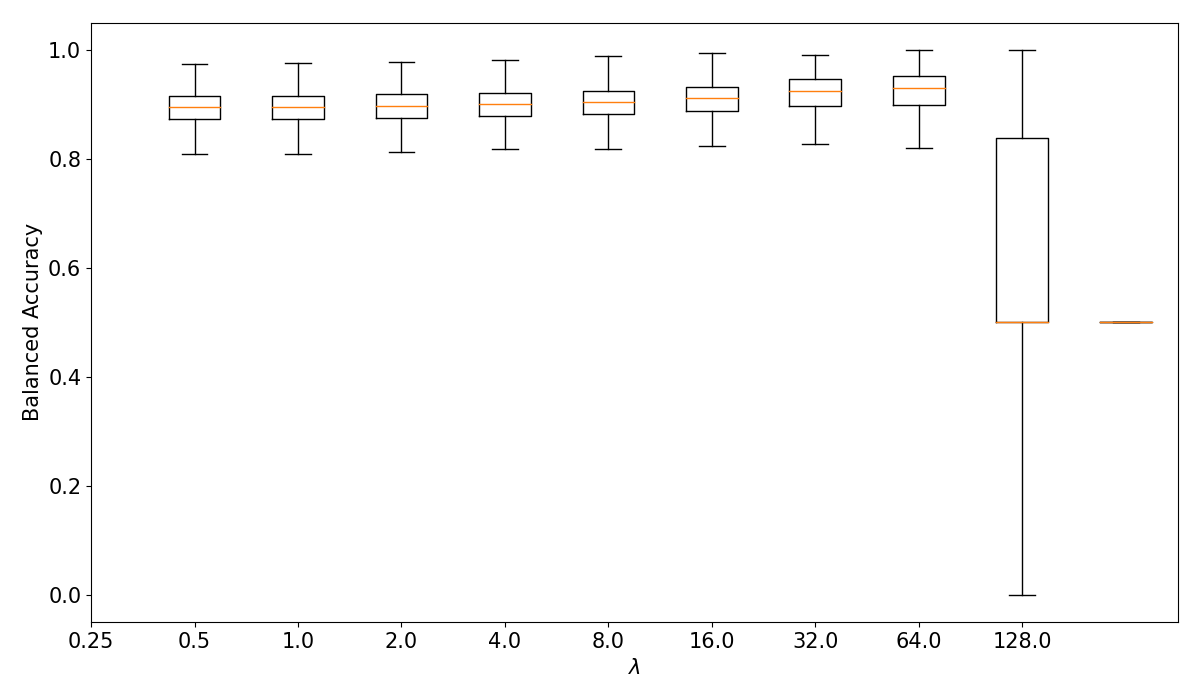
\includegraphics[width=1\textwidth]{analysis/model_convergence/images/jump_penalties_box.png}
    \caption[Boxplot hypertuning the jump penalizer $\lambda$]{Boxplot hypertuning the jump penalizer $\lambda$.}
    %\label{fig:jump_penalties}
\end{figure}

\section{Simulation results}
\label{appendix:model_convergence}

\begin{figure}[H] 
    \centering
    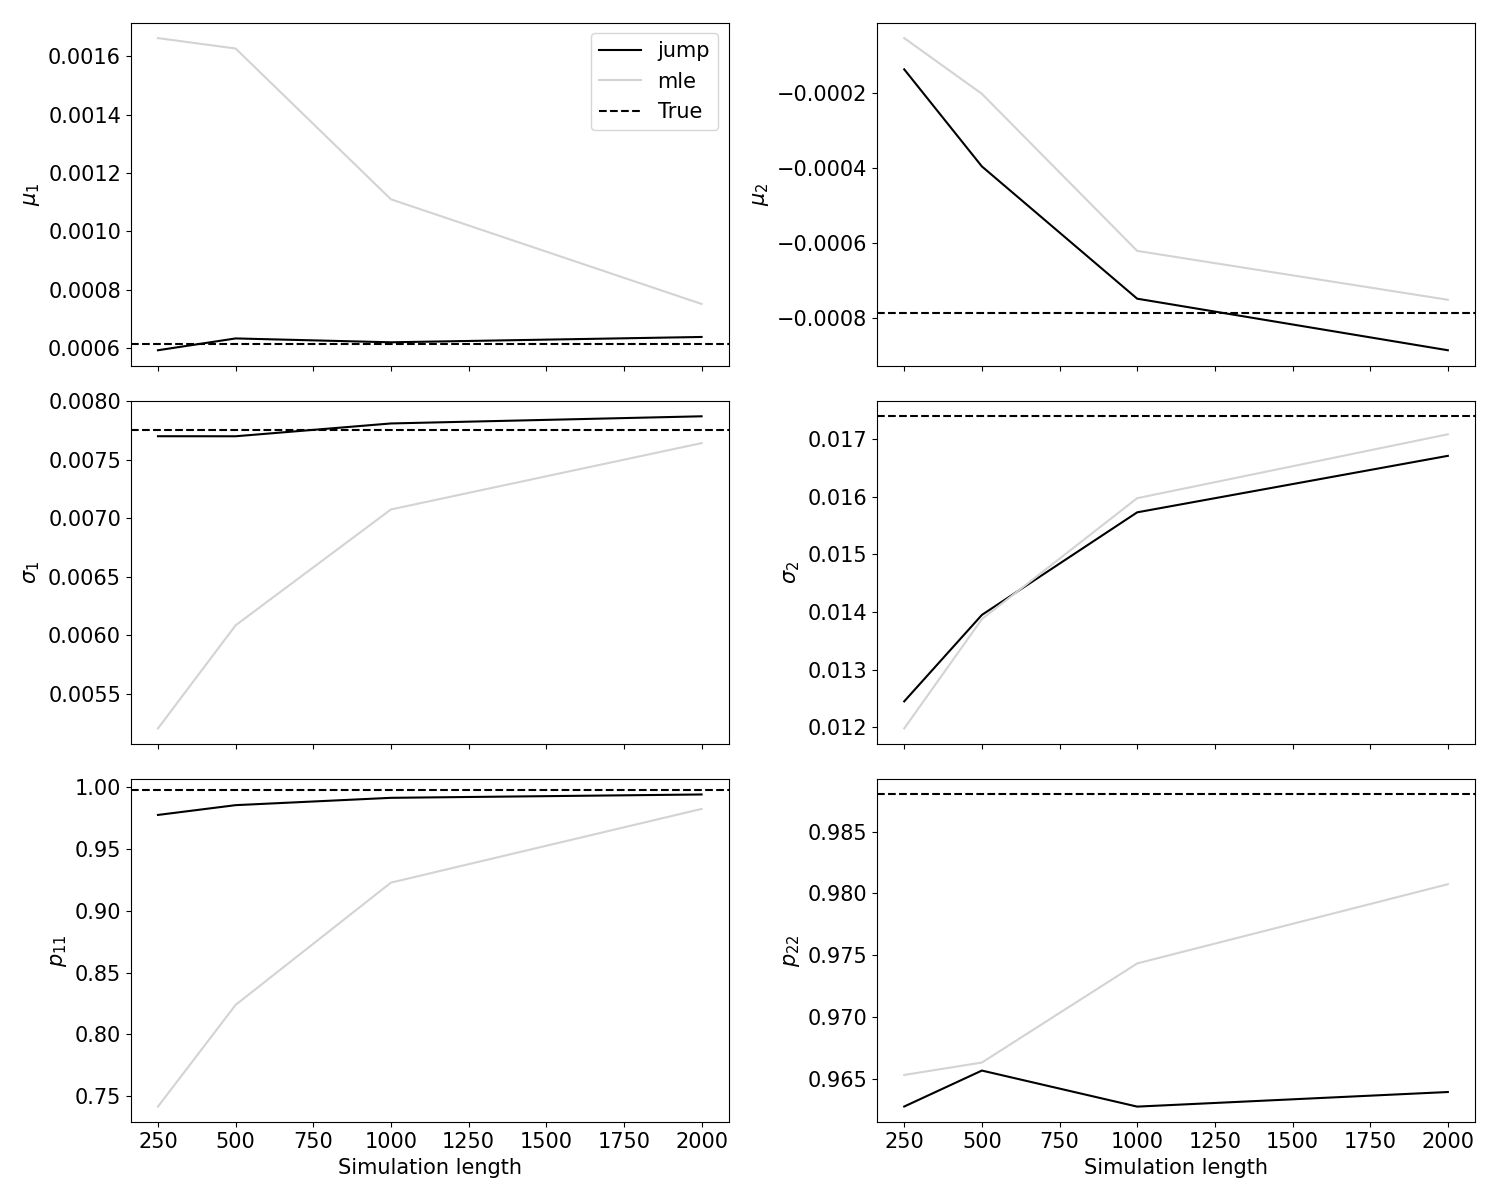
\includegraphics[width=1\textwidth]{analysis/model_convergence/images/simulation_normal.png}
    \caption[Plot of the \mle and \jump parameters, from conditional Gaussian distribution, showing the convergence to the true values]{Plot of the \mle and \jump parameters from conditional Gaussian distributions. The estimates show the models' convergence towards true values as a function of simulation length. Results are based on 1000 simulations.}
    \label{fig:jump_normal}
\end{figure}

\begin{figure}[H] 
    \centering
    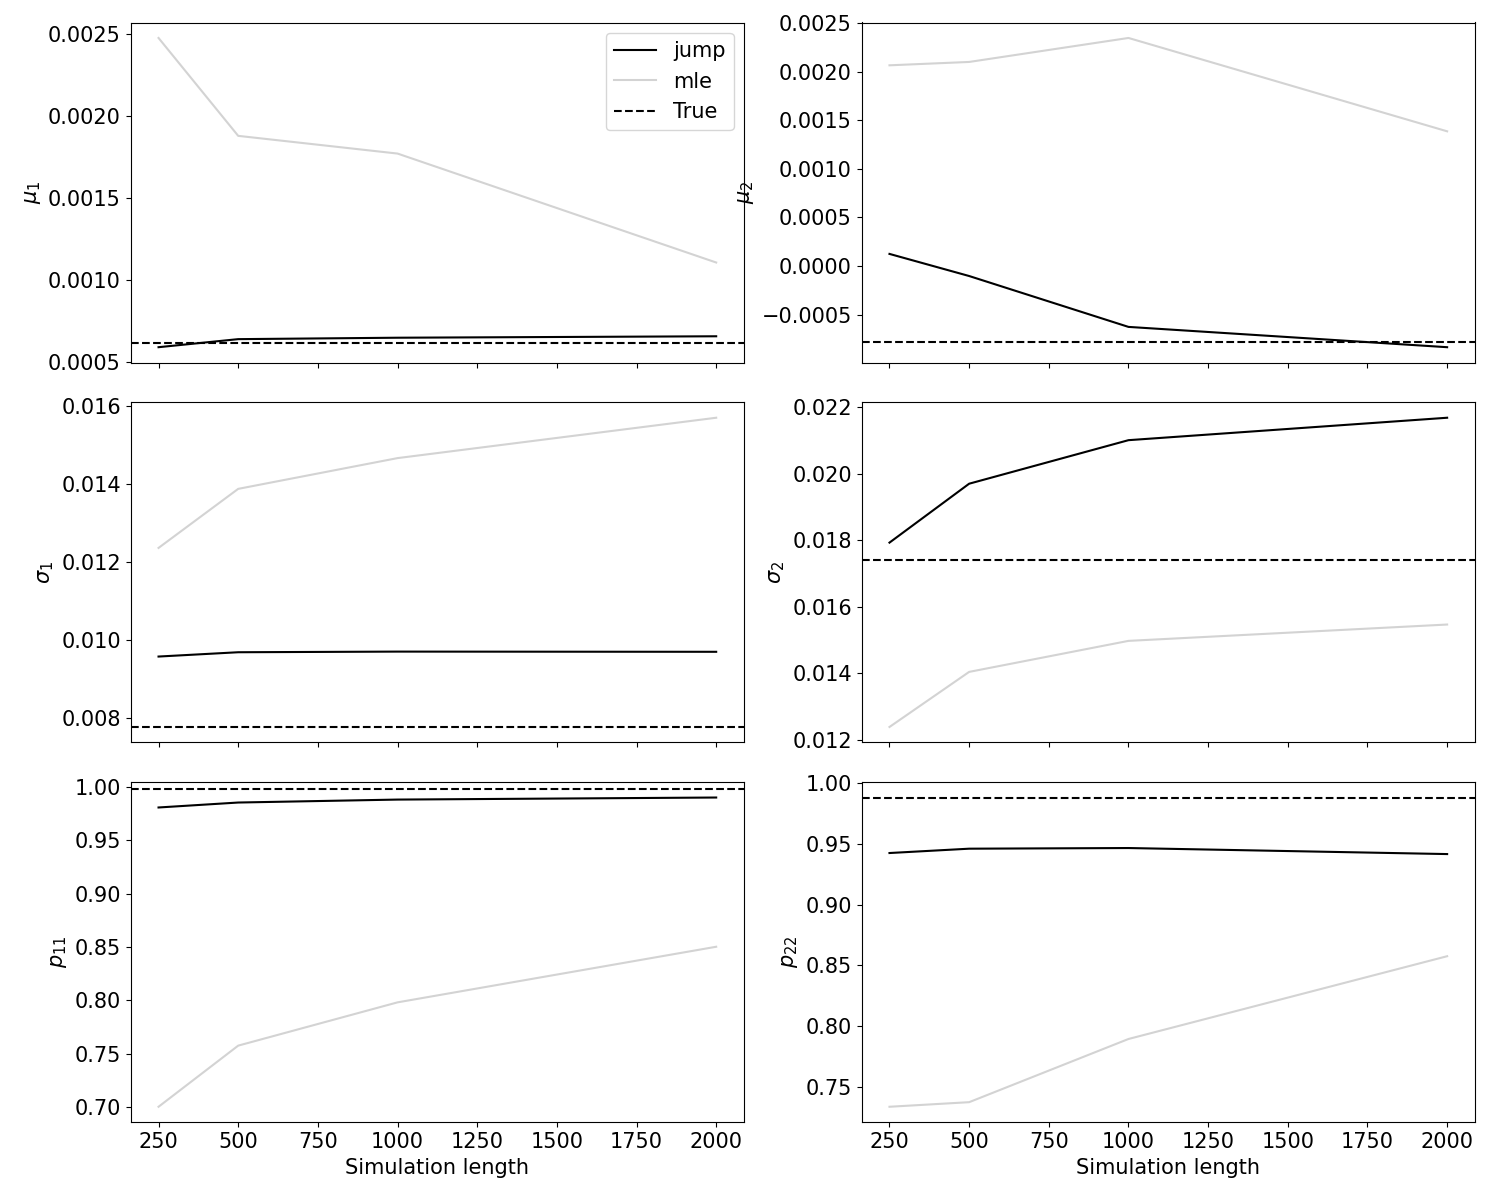
\includegraphics[width=1\textwidth]{analysis/model_convergence/images/simulation_t.png}
    
    \caption[Plot of the \mle and \jump parameters, from conditional t-distributions with five degrees of freedom, showing the convergence to the true values]{Plot of the \mle and \jump parameters from conditional t-distributions with five degrees of freedom. The estimates show the models' convergence towards true values as a function of simulation length. Results are based on 1000 simulations.}
    \label{fig:jump_t}
\end{figure}

\begin{figure}[H] 
    \centering
    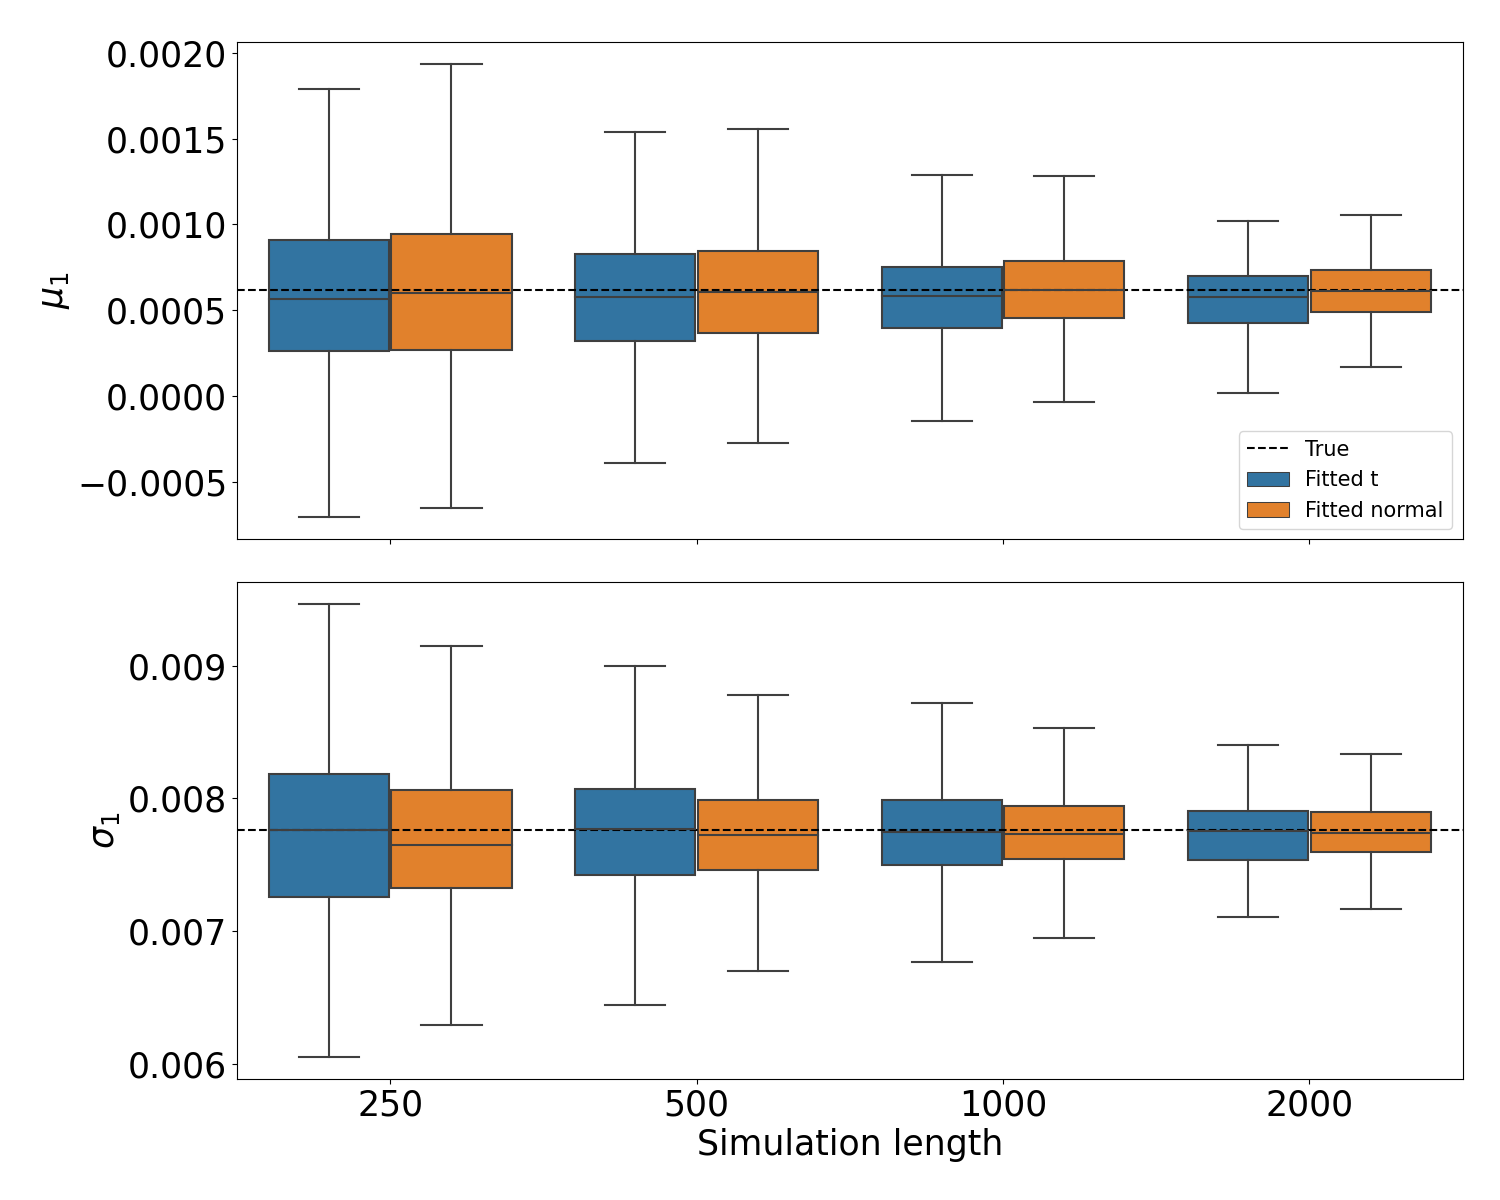
\includegraphics[width=1\textwidth]{analysis/model_convergence/images/theoretical_fit_t_dist.png}
    \caption[Empirical fit of a normal and t-distribution to data simulated from a t-distribution with five degrees of freedom]{Empirical fit of a normal and t-distribution to data simulated from a t distribution with five degrees of freedom. Results are based on 1000 simulated series.}
    \label{fig:jump_theoretical_fit}
\end{figure}

\section{Reproducing TP1 and TP4}
\label{appendix:sign_rt}

\begin{figure}[H] 
    \centering
    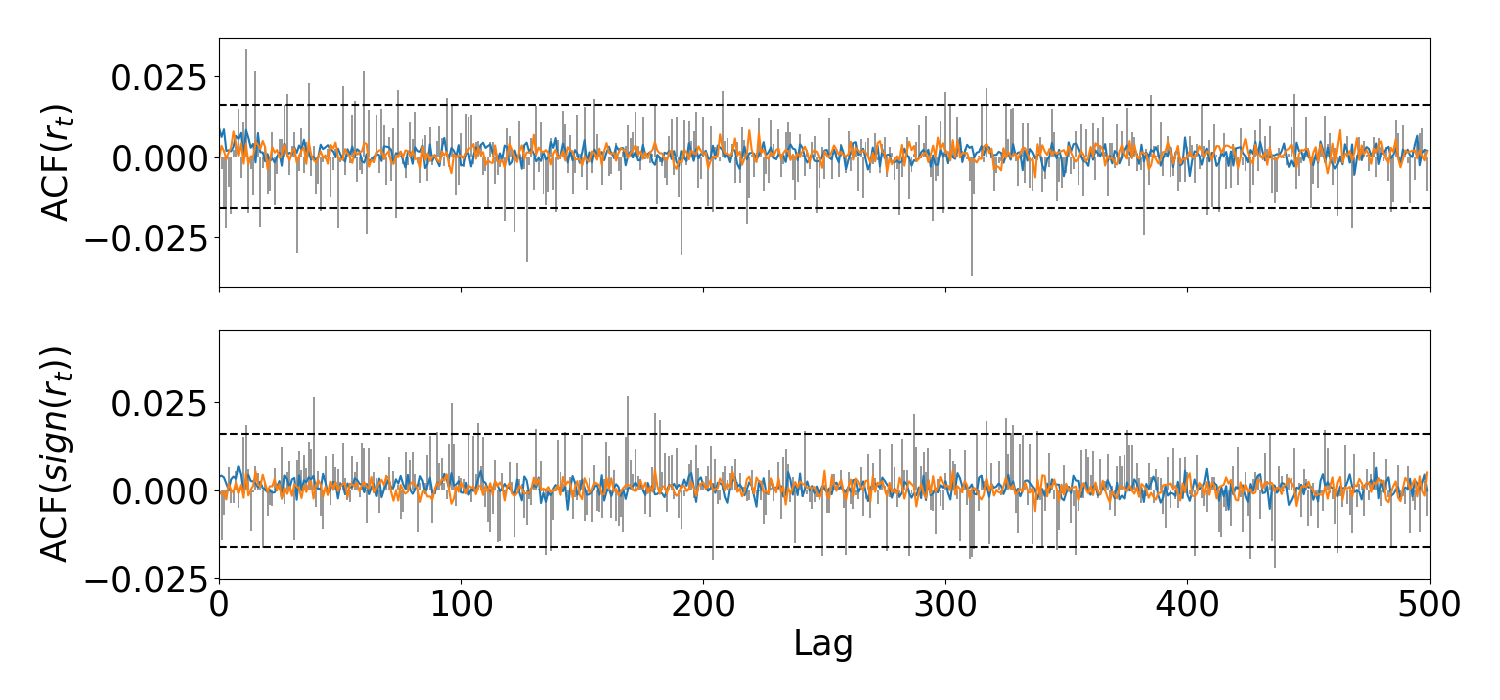
\includegraphics[width=1.0\textwidth]{analysis/stylized_facts/images/acf_sign.png}
    \caption[Autocorrelation function of $r_t$ and $sign(r_t)$]{Autocorrelation function of $r_t$ and $sign(r_t)$.}
    \label{fig:stylized_facts_acf_sign_rt} 
\end{figure}

\section{Outlier corrected rolling moments and ACF plots}

\begin{figure}[H] 
    \centering
    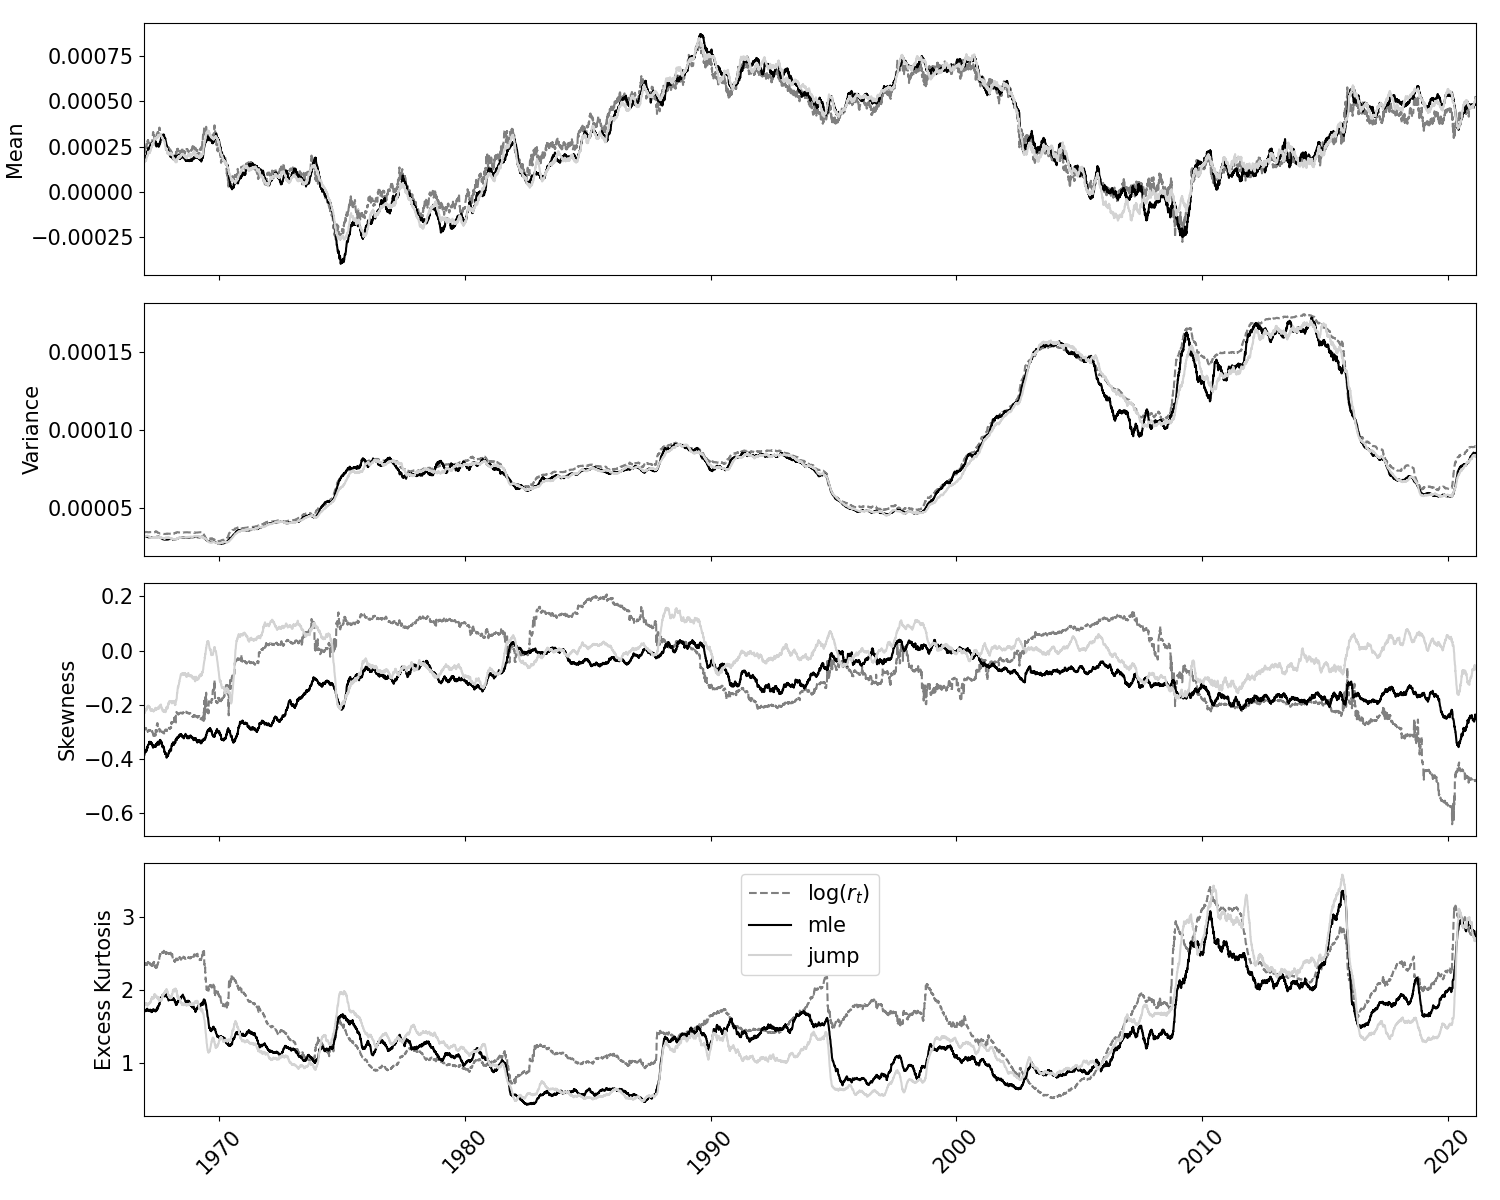
\includegraphics[width=1.0\textwidth]{analysis/stylized_facts/images/moments_outlier_corrected.png}
    
    
    \caption[Development of the first four moments from the estimated models and $r_t$]{Development of first four moments from the estimated models compared to $r_t$ using a rolling window of 1700 days. Model estimates are calculated using Monte-Carlo simulations.}
    
    \caption[Development of the first four moments from the outlier corrected estimated models and $r_t$]{Development of first four moments from the estimated models compared to $r_t$ using a rolling window of 1700 days. Model estimates are calculated using Monte-Carlo simulations correcting for outliers that are further than four standard deviations away from the mean. Outliers are treated locally in each subsample of 1700 observations.}
\label{fig:stylized_facts_rolling_moments_outliers_appendix}
\end{figure}

\begin{figure}[H] 
    \centering
    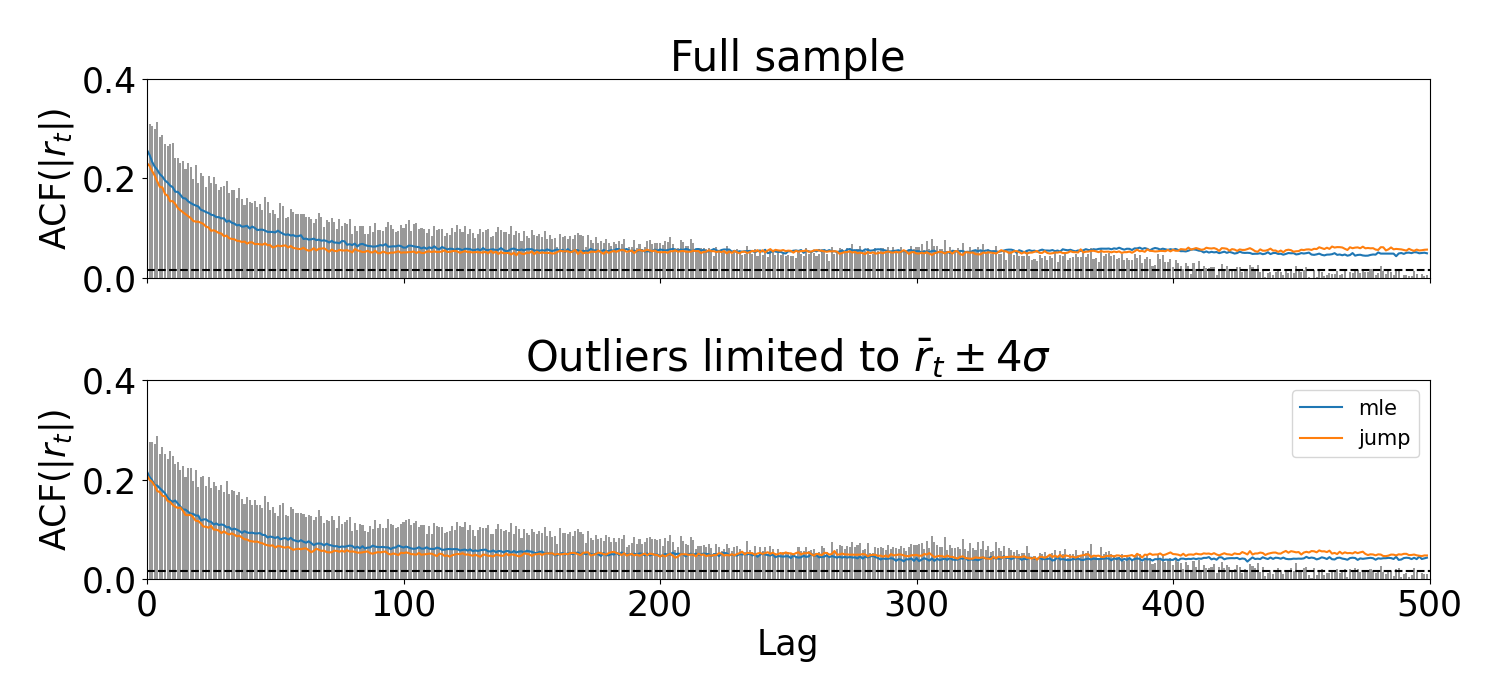
\includegraphics[width=1.0\textwidth]{analysis/stylized_facts/images/acf_abs_outlier.png}
    \caption[Autocorrelation function of $|r_t|$]{Autocorrelation function of $|r_t|$. The panel shows results on the full data and the bottom panel shows results after correcting outliers to $\bar r_t \pm 4\sigma$.}
\label{fig:stylized_facts_acf_abs_outlier}
\end{figure}


From the \cref{fig:stylized_facts_acf_plots_sub_periods}, it is evident that the autocorrelation functions estimated directly from the \mle and \jump model show a much faster decay than the decay of the empirical absolute ACF, thereby confirming the results of both Rýden et al (1998) and Bulla et al. (2011). Despite this property, the autocorrelation function generated by both the \mle and \jump model, does capture the general tendency of the empirical absolute ACF reasonably well, with the exception of the models in sub-period 9 and 10. However, it also appears that the \jump model provide a better fit compared to the model which is estimated through the \mle approach. This is in line with the fact that Bulla et al. (2011) concluded that t-distributed HMMs estimated by the \mle approach provide a superior fit compared to a traditional Gaussian HMM. Even though the thesis neglect the fitting of a t-distribution, the general conclusion that constraining the models either through distributional properties or jump penalizers provide a better fit holds. The neat aspect associated with splitting the the observations of the full sample absolute autocorrelation of the log returns into smaller digestable sub-periods is that the time-varying nature of the absolute autocorrelation of the empirical log returns becomes visible. As such, it appears that the long memory property associated with financial returns is better captured by splitting the full sample data into sub-periods, which in this case is 10. As such, figure \ref{fig:stylized_facts_acf_plots_sub_periods} points towards a similar conclusion as figure \ref{fig:stylized_facts_acf_plots}, since both the \mle and \jump methodology, in general, reproduces volatility clustering quite well. However, there are periods in which the models, and their associated parameters, fail to fit the absolute ACF of the log returns, which could be due to the models being miss-specified for some time-periods due to the rolling estimation procedure as argued for figure \ref{fig: MLE estimation rolling parameters} and \ref{fig: Jump estimation rolling parameters}. 

    %\addcontentsline{toc}{section}{Appendix}
    
    
    
    
\end{document}